%Book style with A4 paper, chapeters start on left page only, using times fonts
\documentclass[12pt,a4paper,oneside]{book}		
\usepackage{pdfpages}

\usepackage{longtable}
\usepackage{tikz}
\usetikzlibrary{trees}

\sloppy

\usepackage[T1]{fontenc} %write accents
\usepackage[utf8]{inputenc} %permits to write the text with accents
% \usepackage[latin1]{inputenc}
\usepackage[spanish]{babel}
%\usepackage{csquotes}
\usepackage[backend=biber, style=ieee]{biblatex}
\addbibresource{referencias.bib}
\addto\captionsspanish{\renewcommand{\tablename}{Tabla}}
\usepackage{adjustbox} 
\usepackage{changepage} %Margin adjustment and detection of odd/even pages
\usepackage{caption}
\usepackage{float}
%paquete de simbulo de marca registrada
\usepackage{textcomp}
%Paquete para códigos de programacion
\usepackage{listings}

%To prepare list of symbols
\usepackage{longtable}
%para colorear celdas de tablas
\usepackage[table]{xcolor}% http://ctan.org/pkg/xcolor
%Ajustar titulos
\usepackage{titlesec}
% Ajustes para el espaciado antes y después de los capítulos
\titlespacing{\chapter}{0pt}{\parskip}{\parskip}
% Personalizar el formato de los capítulos
\titleformat{\chapter}[display]
  {\normalfont\huge\bfseries}{}{0pt}{\Huge}




% Sets the margins of the document.
\oddsidemargin 5mm
\evensidemargin 5mm
\textwidth 150mm
\topmargin 0mm
\headheight 0mm
\textheight 225mm

% Selects font encoding
% \usepackage[T1]{fontenc}
\usepackage{ae,aecompl}
%\usepackage{times}

\usepackage{lipsum}

\usepackage{epigraph}
\setlength{\epigraphrule}{0pt}
\setlength{\afterepigraphskip}{2\baselineskip}

%header displays information according to document class and page number top right.
\usepackage{fancyhdr}


% Starts new paragraphs without indentation but with some space between the new and the previous paragraph.
\usepackage{parskip}
\setlength{\parskip}{1.5ex plus 0.4ex minus 0.4ex}
%\usepackage{indentfirst}

% try to keep paragraphs together
\widowpenalty=300
\clubpenalty=300

% Used to create tables with rows/cols spanning over se
\usepackage{array}
\newcolumntype{L}[1]{>{\arraybackslash}p{#1cm}}
\newcolumntype{C}[1]{>{\centering\arraybackslash}p{#1cm}}
\usepackage{multirow}

%Professional tables
\usepackage{booktabs}

% Math
\usepackage{amssymb}
\usepackage{amsmath}

% Used to include images with the includegraphics command
\usepackage{epsfig,subfigure,amstext}
\usepackage{graphicx}

\usepackage{makeidx}
\makeindex

% use for landscape pages
\usepackage{pdflscape}

%permits relative paths in the imported files
\usepackage{import}

%permits to create different environments
\usepackage{amsthm}

\newtheoremstyle{simple}
   {8pt}% hSpace above
   {}% hSpace below
   {\it}% hBody font
   {1em}% hIndent amount
   {}% hTheorem head font
   {\textup{:}}% hPunctuation after theorem head
   {.7em}% hSpace after theorem head
   {}% hTheorem head spec (can be left empty, meaning `normal')

\newtheoremstyle{enhanced}
   {8pt}% hSpace above
   {}% hSpace below
   {}% hBody font
   {1em}% hIndent amount
   {\itshape}% hTheorem head font
   {\textup{:}}% hPunctuation after theorem head
   {.7em}% hSpace after theorem head
   {}% hTheorem head spec (can be left empty, meaning `normal')


%links in pdf (index, references, and figures..., change the colors to black)
\usepackage[pdfborder={0 0 0},breaklinks=true,bookmarksopen=true,bookmarksopenlevel=1]{hyperref}


% Used to include algorithms
%\usepackage{algorithm,algorithmic}
%\renewcommand{\algorithmiccomment}[1]{\hfill \textit{//#1}}
%\newcommand{\vect}[1]{\overrightarrow{#1}}
%
%------------------------------------------------------------------
\chapter{Simulação Baseada em Eventos Discretos}\label{app:simulacao}
%------------------------------------------------------------------

In discrete-event simulation the system is controlled by events that change the state of the system. A discrete-event simulator has two main components: clock and event list. The clock controls the simulation time, while the event list maintains the list of active events. At any time (simulation time), there is only one event happening. 

The network aspects are simulated as follows. The messages from a node $n_i$ to a node $n_j$ are handled as a message deliver event. The event is schedule to occur in a time in future calculated based on the size of the message in bytes multiplied by the network speed. Thus, the computer behaves as a single instance of the entire system that may have thousands of nodes. For example, assume that we want to execute the plan where each MBR $m_i$ comes from a single node $n_i$. The processing starts at node $n_1$ that process the skyline and selects the filter points. The node $n_1$, than schedule two message deliver events, one to node $n_3$ and another to node $n_2$. The plan delivered to node $n_3$ is composed exclusively by the MBR $m_3$, while the plan delivered to node $n_2$ is composed by $m_2 \rightarrow m_4$. Since the message sent to node $n_3$ is smaller than the message sent to node $n_2$, the message sent to node $n_3$ will be scheduled to a shorter time in future. Thus, the next event to be processed will be message arrived in node $n_3$ that will start processing the skyline of $m_3$ using the filter points received from node $n_1$. If two messages are scheduled for the same simulation time, the simulator chooses any one of them randomly. 

The response time in our simulation is computed getting the maximum transfer time plus local process time. For example, if all transfer messages in the example above took 1 second and the local processing at each node also took 1 second, the response time will be defined by the response time of the longest path. Thus, the response time will be the time to send a message to $m_2$ plus the time to process the local skyline at $n_2$ plus the time to transfer the message to $n_4$  plus the time to compute the local skyline at $n_4$ plus the time to send the result back to $n_2$ plus the time to send the result back to $n_1$. 


\usepackage{tikz}
\usetikzlibrary{trees}
\usepackage{forest}

\begin{document}
\selectlanguage{spanish}
% \selectlanguage{english}

% Define o título da tese.
\def\thesisTitle{Diseño y construcción de una cabina estratosférica con estabilizador para la recolección de datos y contenido multimedia} 

% Defina o nome do(a) autor(a) (é o seu nome).
\def\thesisAuthor{Chávez Urbano Erick, Niño Galindo Pamela Esmeralda, Diego Jimenez Martinez, Tomas Osorio de los Ángeles, Erick López Cruz} 

% Defina o nome do(a) orientador(a) 
\def\thesisAdvisor{Rebeca Hernández} 

% Defina o nome do(a) co-orientador(a) 
% Comente a linha abaixo se não tiver coorientador 
\def\thesisCoAdvisor{Nome do(a) Coorientador(a)} 

\pagestyle{empty}

\begin{titlepage}
\begin{center}



\includegraphics[width=40mm]{cover/utm.png} \\

\large

\textbf{Universidad Tecnológica de la Mixteca}

\vspace{.5cm}
\large
\textbf{Estudio de mercado para la comercialización de cabinas climatizadas en la ciudad de Oaxaca} 

\vspace{.5cm}

\huge{\ \textbf{TerraGreen: Desarrollo de ambientes controlados} }

\vspace{.5cm}

\large
Décimo semestre

Ingeniería mecatrónica

Segundo parcial

\Large
\textbf{Presentan:}

Erick Chávez Urbano

Jiménez Martínez Diego

Niño Galindo Pamela Esmeralda

Osorio de los Ángeles Tomás

López Cruz Erick

\vfill

\large
\textbf{Docente: M.A.N. Rebeca Hernández}

\textbf{Av. Modesto Seara, Acatlima, Huajuapan de León, Oaxaca, México}

\textbf{Abril \the\year}

\end{center}
\end{titlepage}



%------------------------------------------------------------------------------%
%%%%%%% Second page
%------------------------------------------------------------------------------%
 



%\null
\vfill

\begin{center}
	\textit{Está página deverá ser substituída por uma folha contendo as assinaturas dos membros da banca, e deve ser colocada após a ficha catalográfica}
\end{center}
 

% Includes page number at the bottom of the page.
\pagestyle{plain}

% Uses small roman numbers for page numbering.
\pagenumbering{arabic} 				

% Resets the page counter to 1.
\setcounter{page}{1}

%\chapter*{Abstract}
\addcontentsline{toc}{chapter}{Abstract}

The abstract in English. \lipsum[3]

\vspace{.5cm}

\textbf{Keywords:} keyword1, keyword2, ...

%\chapter*{Resumo}
\addcontentsline{toc}{chapter}{Resumo}

Texto do resumo em português. \lipsum[1]

\vspace{.5cm}

\textbf{Palavras-chave:} palavra-chave, palavra-chave2, ...
 
%\chapter*{Prefácio}
\addcontentsline{toc}{chapter}{Prefácio}

Esta dissertação de mestrado foi submetida à Universidade Federal da Paraíba (UFPB) como requisito parcial para obtenção do grau de Mestre em Informática. 

A dissertação foi desenvolvida no Programa de Pós-Graduação em Informática (PPGI),  tendo como orientador o Prof. Dr. \textbf{\thesisAdvisor}.
\ifdefined\thesisCoAdvisor
O Prof. Dr. \textbf{\thesisCoAdvisor} foi coorientador(a) deste trabalho. 
\fi

Esta pesquisa foi financiada pela FAPESB (ou CAPES). \textit{Obrigatório colocar esse texto, caso o(a) estudante tenha recebido bolsa da FAPESB (ou da CAPES).}

\cleardoublepage 
%\chapter*{Agradecimentos}
\addcontentsline{toc}{chapter}{Agradecimentos}

Colocar o texto dos agradecimentos aqui. 

\cleardoublepage 
%\vspace*{15cm}

\epigraph{\it ``Com grandes poderes, vêm grandes responsabilidades.''}{-- Tio Ben}

\cleardoublepage % opcional 


%Prints the table of contents
\renewcommand{\contentsname}{Índice}
\tableofcontents
%\addcontentsline{toc}{chapter}{Sumário}

% Prints a list of tables
\listoftables					
\addcontentsline{toc}{chapter}{Índice de tablas}
\clearpage


% Prints a list of figures
\listoffigures									
\addcontentsline{toc}{chapter}{Índice de figuras}
\cleardoublepage

\clearpage

% Describes the research line and how the thesis is related with it 
%\chapter*{Alinhamento com a Linha de Pesquisa} 
\addcontentsline{toc}{chapter}{Alinhamento com a Linha de Pesquisa}

% - Seção Alinhamento com as linhas de pesquisa (nome da linha e breve descrição de como a dissertação está alinhada).

% Descomentar o parágrafo com a linha de pesquisa da sua dissertação.
\textbf{Linha de Pesquisa: Software e Sistemas Computacionais}
% \textbf{Linha de Pesquisa: Computação Inteligente}

\vspace{1cm}

Descrever brevemente como a dissertação está alinhada com a linha de pesquisa.

% - Seção Produções bibliográficas e técnicas resultantes e prêmios (lista de produções e relevância destas produções)
% - Seção Alinhamento com as linhas de pesquisa; (nome da linha e breve descrição de como a dissertação está alinhada)


% Prints a list of prizes and bibliographic and technical production 
%\chapter*{Produções Bibliográficas, Produções Técnicas e Premiações} 
\addcontentsline{toc}{chapter}{Produções Bibliográficas, Produções Técnicas e Premiações}

% - Seção Produções bibliográficas e técnicas resultantes e prêmios (lista de produções e relevância destas produções)

Listar as produções bibliográficas e técnicas do autor durante o mestrado, além de destacar eventuais premiações obtidas durante a dissertação (e.g., melhor artigo em evento, premiação em concurso de inovação, etc.).


% Fancing heading alternating section and chapter with page count on the top
\pagestyle{fancy}
\fancyhead[LE,RO]{\thepage} 
\fancyhead[RE,LO]{\nouppercase{\leftmark}} 
\setlength{\headheight}{14.5pt}
\cfoot{}

\pagenumbering{arabic} 				
% Uses arabic numbers (normal numbers) for page numbering.

\setcounter{page}{1}
% Resets the page counter to 1.

% The chapters
\chapter{Introducción}

La industria florícola enfrenta desafíos significativos relacionados con la conservación y el mantenimiento de la calidad de las flores desde su cultivo hasta su comercialización. En este contexto, las cámaras climáticas se presentan como una solución innovadora y eficaz para asegurar las condiciones óptimas de temperatura, humedad y luz necesarias para preservar la frescura y prolongar la vida útil de las flores. Este proyecto empresarial tiene como objetivo desarrollar y evaluar un sistema de cámaras climáticas especializado en flores, abordando aspectos cruciales como el estudio de mercado, el estudio técnico, el estudio administrativo-legal y el estudio económico.

El estudio de mercado se centrará en analizar la demanda actual y futura de cámaras climáticas en la industria florícola, identificando las necesidades específicas de los productores y comerciantes de flores, así como las tendencias y oportunidades del mercado. Este análisis permitirá definir la viabilidad comercial del proyecto y diseñar estrategias efectivas de penetración y posicionamiento en el mercado.

El estudio técnico evaluará las especificaciones y requerimientos tecnológicos necesarios para el desarrollo de las cámaras climáticas, considerando factores como la ingeniería de diseño, los materiales, la eficiencia energética y la automatización de los sistemas de control ambiental. Además, se realizarán pruebas y simulaciones para garantizar el rendimiento y la fiabilidad de las cámaras en diferentes condiciones operativas.

El estudio administrativo-legal abordará la estructura organizativa y los aspectos jurídicos relacionados con la implementación del proyecto, incluyendo la constitución legal de la empresa, los permisos y licencias necesarios, las normativas ambientales y de seguridad, y la gestión de recursos humanos. Este análisis garantizará el cumplimiento de todas las regulaciones y normativas aplicables, minimizando riesgos legales y administrativos.

El estudio económico, acompañado de una evaluación económica detallada, analizará los costos y beneficios asociados al desarrollo y operación de las cámaras climáticas, proyectando ingresos, gastos, flujos de caja y rentabilidad a corto y largo plazo. Esta evaluación permitirá determinar la viabilidad financiera del proyecto y su potencial de retorno de inversión, proporcionando una base sólida para la toma de decisiones estratégicas.

En resumen, este proyecto empresarial tiene como objetivo ofrecer una solución integral y efectiva para la industria florícola mediante el desarrollo de cámaras climáticas avanzadas, asegurando su viabilidad técnica, comercial, administrativa y económica. Con un enfoque multidisciplinario y un análisis exhaustivo en cada uno de los estudios mencionados, buscamos contribuir al crecimiento sostenible y a la competitividad del sector florícola


\chapter{Estudio de mercado}

El estudio de mercado es esencial para comprender el entorno y tomar decisiones estratégicas en el desarrollo y comercialización de cabinas climatizadas para su aplicación en plantas. Esta introducción da una visión del contexto en el que se realizó la investigación y establece la relevancia de los hallazgos del estudio.

\textbf{La realización de este estudio surge de la necesidad de:}

\begin{itemize}
    \item Evaluar la viabilidad y demanda de las cabinas climatizadas para plantas en el mercado local.
    \item Identificar las necesidades y preferencias de los consumidores interesados en este tipo de productos.
\end{itemize}

\textbf{Objetivo del Estudio de Mercado}

El objetivo específico del estudio de mercado es obtener información sobre el mercado objetivo, identificar el perfil del público interesado y evaluar la relación entre oferta y demanda de las cabinas climatizadas para plantas en la región de Valles Centrales de Oaxaca de Juárez. 

\section{Definición y descripción del producto}

Las cabinas climatizadas para plantas son espacios cerrados diseñados para mantener condiciones específicas de temperatura, radiación UV y humedad. 

\textbf{Características}
\begin{itemize}
    \item Diseño Modular: Las cabinas se fabrican con paneles prefabricados para que se puedan añadir accesorios.
    \item Climatización: Control preciso de la temperatura y humedad mediante sistemas de aire acondicionado y calefacción.
    \item Aislamiento: Paneles con alto aislamiento térmico para mantener condiciones internas estables.
    \item Iluminación Interna: Incorporan sistemas de iluminación para facilitar el trabajo en su interior.
\end{itemize}

\textbf{Ventajas}
\begin{itemize}
    \item Espacio Personalizado: Se pueden instalar en áreas específicas sin necesidad de climatizar todo el lugar.
    \item Ahorro de Energía: Eficiencia energética al mantener condiciones óptimas sin desperdiciar recursos.
    \item Comodidad y seguridad: Protección contra condiciones climáticas extremas.
    \item Flexibilidad: Adaptación a diferentes usos, como oficinas, zonas de almacenamiento o salas de control.
\end{itemize}

\textbf{Desventajas}
\begin{itemize}
    \item Costo Inicial: La inversión inicial puede ser alta debido a la tecnología y materiales utilizados.
    \item Mantenimiento: Requieren mantenimiento para asegurar su funcionamiento óptimo, aunque este no sea frecuente.
    \item Dependencia de Energía: Necesitan fuentes de energía para la climatización.
\end{itemize}

\subsection{Análisis de la materia prima }
La materia prima para la elaboración de las cabinas climatizadas para el desarrollo de las plantas cuenta de una diversidad de componentes, en su mayoría de naturaleza electrónica, a continuación, se presenta un listado de materiales a usar y su costo comercial. 

\begin{table}[H]
\centering
\caption{Lista de materiales}
\begin{tabular}{|p{4cm}|p{3cm}|p{3cm}|p{3cm}|}
\hline
\textbf{Materia prima utilizada}
&\textbf{Costo por unidad} &\textbf{Unidades utilizadas} &\textbf{Costo total}\\
\hline
Hoja de madera 1.5m x 2m & 950 & 1 &950\\
\hline
Acrílico & 750 & 1 & 750\\
\hline
Bisagras & 75 & 2 & 150\\
\hline
Tornillos & & & 200\\
\hline
Pegamento & 120 & 1 &120\\
\hline
ESP32 & 200 &1 &200\\
\hline
ESP32 CAM &200&1 &200\\
\hline
DHT11&60 &x &60x\\
\hline
Relés & 40 & x & 40x \\
\hline
Motor & 600 & 1 &600\\
\hline
Display Oled 128x64 & 90&1&90\\
\hline
RTC&135&1&135\\
\hline
Puente H&55&1&55\\
\hline
Ultrasónico&35&2&70\\
\hline
Celda peltier&425&x&425x\\
\hline
Buzzer&35&1&35\\
\hline
\end{tabular}
\label{tabla:piezasSoporteEstabilizador}
\end{table}

\section{Análisis de la demanda}
Estas cabinas forman parte de una línea especifica de productos relacionados con la jardinería. Los consumidores que estén interesados en el cultivo de las plantas en interiores o espacios limitados pueden buscar dichas cabinas como una solución práctica.

\section{Definición del mercado}

El mercado meta es la población de las principales ciudades y destinos turísticos del estado de Oaxaca, de sexo indistinto que perciban salarios medios a altos y que tengan como pasatiempo o trabajo el cuidado de plantas.

Este grupo incluye a los amantes de la jardinería, propietarios de viviendas con espacio para plantas y personas interesadas en plantas de interior.
Las empresas de jardinería, viveros y tiendas especializadas pueden ser parte del mercado. Estos negocios pueden adquirir cabinas para ofrecer a sus clientes o utilizarlas para el cultivo de plantas en sus instalaciones.

Oaxaca es un destino turístico popular, y las cabinas para el cuidado de las plantas podrían ser atractivas para hoteles y alojamientos que deseen proporcionar un ambiente verde y relajante para sus huéspedes.

\subsection{Tamaño de la muestra}
Para calcular el tamaño de la muestra necesaria para obtener resultados certeros, se utiliza la siguiente fórmula:

\[
n = \frac{{\sigma^2 Upq}}{{e^2 (U - 1) + \sigma^2 pq}}
\]

Donde:

U = 1496300 (población de Oaxaca con ingresos mayores al mínimo)
{\sigma = 1.96} \textit{(Coeficiente de confianza)}

\[
p = 0.5, q=0.5, e = 0.05
\]

Teniendo como resultado 

\[
n = 384 \textit{ respuestas}
\]

El tamaño del universo U     se tomó de la población que no se encuentra en algún estado de pobreza en la población del estado, siendo la fuente principal el CONEVAL \cite{Coneval}.

\begin{figure}[H]
    \centering	
    \includegraphics[width=.8\textwidth]{img/Empresa/Población 2020.jpg} 
    \caption{Medición de pobreza 2020}
\label{fig:MedicionPobreza2020}
\end{figure}

\subsection{Proyección de la demanda }
Los datos analizados para poder proyectar la demanda contienen información recopilada del INEGI \cite{Censo2020} \cite{INEGIOaxaca} y el CONEVAL. Además, algunos de los datos principales recabados por la encuesta se encuentran en anexos.

\begin{table}[h]
\centering
\begin{tabular}{|c|c|c|}
\hline
\textbf{AÑO} & \textbf{X} & \textbf{Y (Millones de habitantes)} \\
\hline
1900 & 1 & 0.9 \\
1910 & 2 & 1 \\
1921 & 3 & 1 \\
1930 & 4 & 1.1 \\
1940 & 5 & 1.2 \\
1950 & 6 & 1.4 \\
1960 & 7 & 1.7 \\
1970 & 8 & 2 \\
1980 & 9 & 2.4 \\
1990 & 10 & 3 \\
2000 & 11 & 3.4 \\
2010 & 12 & 3.8 \\
2020 & 13 & 4.1 \\
\hline
\end{tabular}
\caption{Tabla de población del estado de Oaxaca (INEGI)}
\label{tab:tablaPoblacionOaxaca}
\end{table}

\begin{figure}[H]
    \centering	
    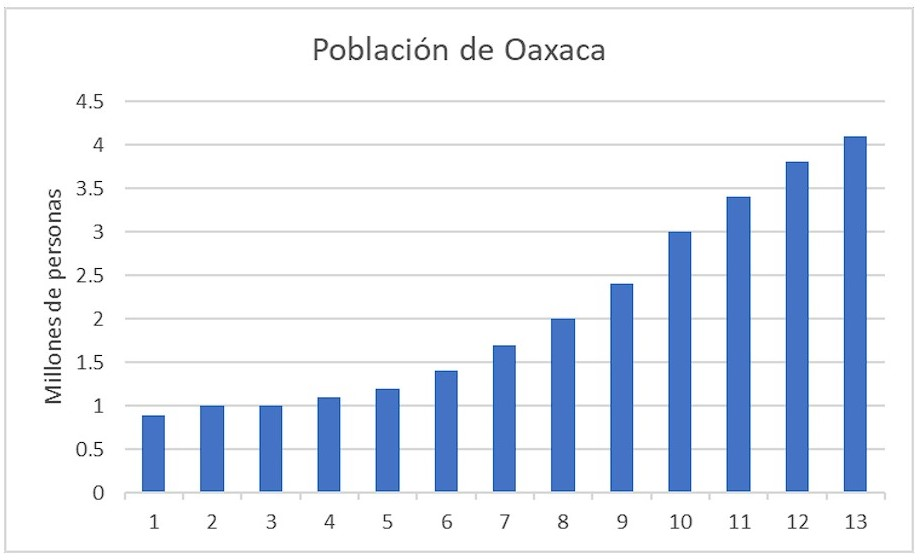
\includegraphics[width=.8\textwidth]{img/Empresa/GraficaPoblacion.jpg} 
    \caption{Gráfica de la población}
\label{fig:GraficaPoblacionOaxaca}
\end{figure}

Debido a que los datos del adquiridos por el CONEVAL empiezan desde el 2008 se extrapolaron datos en los intervalos necesarios para tener una mejor resolución de los datos.

\begin{table}[h]
\centering
\begin{tabular}{|c|c|c|}
\hline
\textbf{AÑO} & \textbf{X} & \textbf{Y (Millones de habitantes)} \\
\hline
2000 & 1 & 3.4 \\
2002 & 2 & 3.48 \\
2004 & 3 & 3.56 \\
2006 & 4 & 3.64 \\
2008 & 5 & 3.72 \\
2010 & 6 & 3.8 \\
2012 & 7 & 3.86 \\
2014 & 8 & 3.92 \\
2016 & 9 & 3.98 \\
2018 & 10 & 4.04 \\
2020 & 11 & 4.1 \\
2022 & 12 & 4.19 \\
2024 & 13 & 4.26 \\
2026 & 14 & 4.33 \\
2028 & 15 & 4.40 \\
2030 & 16 & 4.47 \\
\hline
\end{tabular}
\caption{Tabla de población extrapolada}
\label{tab:PoblacionExtrapolada}
\end{table}

\begin{figure}[H]
    \centering	
    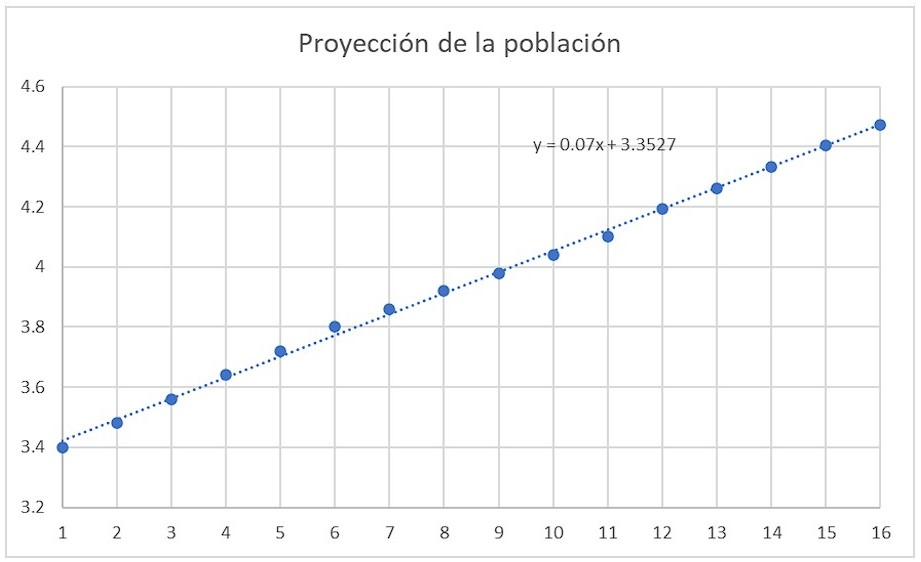
\includegraphics[width=.8\textwidth]{img/Empresa/PosibleCrecimientoPoblacional.jpg} 
    \caption{Gráfica de posible crecimiento poblacional}
\label{fig:GraficaPoblacionOaxacaAprox}
\end{figure}

Sin embargo, según los últimos reportes de la CONEVAL, los índices de pobreza y pobreza extrema en el estado rondan el 60\%, sin embargo, no estar en situación de pobreza no es suficiente para poder adquirir nuestro producto, así que nos enfocamos en la parte de la población que no se encuentra en ningún tipo de pobreza ni vulnerabilidad. Según el último reporte de la CONEVAL, esta parte de la población representa el 23.5\% (tercera columna).
Además, el análisis de la encuesta realizada arroja que el 40\% de las personas encuestadas tienen problemas al cuidar sus plantas, delimitando de mejor manera el mercado objetivo (cuarta columna).

\begin{table}[h!]
\centering
\begin{tabular}{|c|c|c|c|c|}
\hline
\textbf{AÑO} & \textbf{X} & \textbf{Millones de habitantes} & \textbf{No pobres ni vulnerables} & \textbf{Posibles consumidores} \\
\hline
2008 & 1 & 3.72 & 0.7 & 0.28 \\
2010 & 2 & 3.8 & 0.76 & 0.30 \\
2012 & 3 & 3.86 & 0.76 & 0.31 \\
2014 & 4 & 3.92 & 0.8 & 0.32 \\
2016 & 5 & 3.98 & 0.9 & 0.36 \\
2018 & 6 & 4.04 & 0.96 & 0.38 \\
2020 & 7 & 4.1 & 0.96 & 0.39 \\
2022 & 8 & 4.19 & 1.04 & 0.42 \\
2024 & 9 & 4.26 & 1.09 & 0.44 \\
2026 & 10 & 4.33 & 1.15 & 0.46 \\
2028 & 11 & 4.4 & 1.21 & 0.48 \\
2030 & 12 & 4.47 & 1.27 & 0.51 \\
\hline
\end{tabular}
\caption{Evolución de la población y posibles consumidores}
\label{tab:my_label}
\end{table}


\begin{figure}[H]
    \centering	
    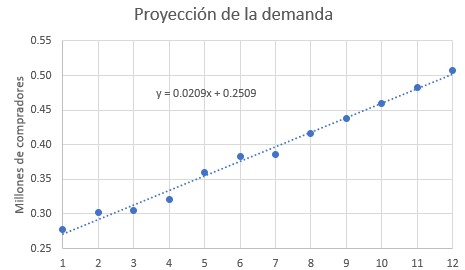
\includegraphics[width=.8\textwidth]{img/Empresa/ProyeccionDemanda.jpg} 
    \caption{Gráfica de proyección de la demanda}
\label{fig:GraficaProyeccionDemanda}
\end{figure}

En conclusión, según la proyección de la demanda, se esperan vender 280,000 unidades para el primer año.

\section{Análisis de la oferta }

En estas cabinas hechas para el ámbito de la jardinería se debe evaluar el marcado y competencia para determinar la demanda y viabilidad del proyecto

\textbf{Evaluación del mercado}
El mercado de cabinas automatizadas para el cuidado de plantas es un nicho emergente en México. Estas cabinas ofrecen soluciones innovadoras para el cultivo y mantenimiento de plantas en entornos controlados. Pese a su potencial, enfrentan desafíos significativos por la falta de productores locales y servicios de mantenimiento. En este informe, exploraremos en detalle la situación actual del mercado y las posibles estrategias para su desarrollo.


\textbf{Oferta actual}

\textbf{Equipos semi automatizados en línea:}

Existen opciones de cabinas semi automatizadas disponibles en páginas de internet. Estos equipos ofrecen funciones básicas como iluminación programable, riego automático y control de temperatura. Sin embargo, su alcance es limitado y no cumplen con los estándares de una cabina completamente automatizada.
La mayoría de estos equipos son importados y no se fabrican localmente en México.

\textbf{Ausencia de productores locales:}

A pesar de la creciente demanda, no existen productores especializados en la fabricación de cabinas para el cuidado de plantas en México.
La falta de producción local dificulta la disponibilidad, personalización y adaptación a las necesidades específicas del mercado mexicano.

\textbf{Demanda y oportunidades}

\textbf{Creciente interés en la jardinería interior:}

La tendencia hacia la jardinería interior y la decoración con plantas ha aumentado en los últimos años. Cada día se realizan 3 mil millones de búsquedas en Google. El 20\% de esas búsquedas son inéditas. En promedio se realizan 135,000 búsquedas al mes con enfoque en plantas, basados en datos de answer the public.

\begin{figure}[H]
    \centering	
    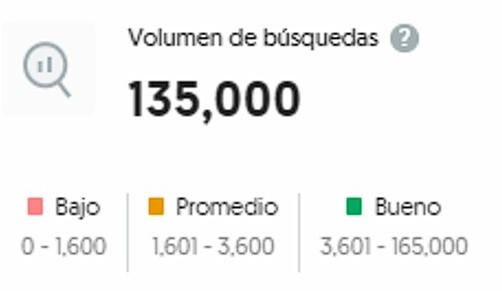
\includegraphics[width=.4\textwidth]{img/Empresa/VolumenBusquedas.jpg} 
    \caption{Volumen de búsquedas sobre jardinería en internet}
\label{fig:GraficaProyeccionDemanda}
\end{figure}

En general las personas buscan soluciones prácticas y estéticas para mantener sus plantas en espacios reducidos.

\textbf{Mercado potencial:}

El mercado objetivo incluye a entusiastas de la jardinería, propietarios de viviendas, oficinas, restaurantes y hoteles.
La conciencia ambiental y la búsqueda de soluciones sostenibles también impulsan la demanda.

\textbf{Necesidad de mantenimiento y reparación:}

Las cabinas automatizadas requieren mantenimiento regular para garantizar su funcionamiento óptimo.
La falta de servicios de mantenimiento y reparación es una barrera para la adopción masiva.

\textbf{Estrategias y propuestas}

\textbf{Fomentar la producción local:}

Se deben incentivar iniciativas para desarrollar productores locales que fabriquen cabinas de alta calidad.
Esto incluye la capacitación en diseño, fabricación y control de calidad.

\textbf{Alianzas con instituciones educativas y centros de investigación:}

Colaborar con universidades y centros de investigación para impulsar la innovación en el diseño y fabricación de cabinas.
Establecer programas de investigación y desarrollo para mejorar la tecnología y la eficiencia.

\textbf{Servicios de mantenimiento y reparación:}

Fomentar la creación de servicios especializados en mantenimiento y reparación de cabinas automatizadas.
Capacitar técnicos y establecer redes de soporte para atender las necesidades de los usuarios.

\textbf{Desafíos del mercado}

\textbf{Escasez de productores locales:}

Uno de los principales desafíos es la falta de productores especializados en la fabricación de cabinas para el cuidado de plantas en México.
La mayoría de las opciones disponibles son importadas, lo que dificulta la adaptación a las necesidades específicas del mercado local.

\textbf{Complejidad tecnológica:}

Las cabinas automatizadas requieren tecnología avanzada para controlar factores como la iluminación, la humedad y la temperatura.
La falta de conocimiento técnico y experiencia en la fabricación de estas cabinas puede ser un obstáculo.

\textbf{Costos iniciales y percepción del valor:}

Las cabinas automatizadas pueden tener un costo inicial significativo.
Convencer a los consumidores de su valor a largo plazo y beneficios sostenibles es un desafío importante.

El mercado de cabinas para el cuidado de plantas en México está en una etapa de crecimiento y transformación. Aprovechar las oportunidades y superar los desafíos requerirá una colaboración activa entre los diferentes actores involucrados. La inversión en investigación, desarrollo y educación será clave para satisfacer la creciente demanda de soluciones sostenibles en la jardinería interior.

\section{Análisis de precio}

El siguiente análisis de precios tiene como finalidad realizar la investigación necesaria para conocer los precios actuales en el mercado local, estatal e internacionalmente, ya que hoy se puede conseguir un producto similar por varios medios. Para esta investigación se estudiaron a los diferentes competidores y se realizó el análisis para establecer precios y lineamientos en los diferentes intermediarios que se establecieron.  

Para recabar la información de la competencia se investigó a la competencia y se realizó el siguiente análisis de datos. El análisis de precios siguió una técnica parecida la presentada en \cite{Gonzalez}. 

\textbf{Precios de los productores a los intermediarios:}

Para estudiar a la competencia que ofrezca un producto similar dentro de la zona que distribuiremos, no hay establecimiento al que se pueda estudiar, pero no solo hay competidores locales a los que se investigó, también hay competidores nacionales e internacionales con los que se puede comparar, ya que, aunque no se encuentran como tal en la localidad, si son parte de la competencia al poder vender y entregar un producto similar en la misma localidad donde estamos. 
El producto que ofrecen es directamente entre vendedor y comprador, a diferencia de nosotros, siendo los primeros en el territorio local podemos fijar el precio a nuestros clientes intermediarios, para analizar primero los precios de la competencia entre vendedor y comprador final. 

\textbf{Precios de los productores a los clientes finales:}

El precio que ofrece directamente AliExpress \cite{AliExpress} a los clientes finales es

\begin{table}[h!]
\centering
\begin{tabular}{|l|l|l|r|}
\hline
\multicolumn{2}{|c|}{\textbf{PRODUCTO}} & \textbf{TAMAÑO} & \textbf{PRECIO} \\ \hline
\multirow{2}{*}{Vendedor A} & Cámara climática, Tipo A & 120*165*115 & \$3442 \\
                            & Cámara climática, Tipo B & 130*170*125 & \$16088 \\ \hline
\multirow{2}{*}{Vendedor B} & Cámara climática, Tipo A & 120*165*115 & \$3613 \\
                            & Cámara climática, Tipo B & 130*170*125 & \$14455 \\ \hline
\multirow{2}{*}{Vendedor C} & Cámara climática, Tipo A & 120*165*115 & \$3322 \\
                            & Cámara climática, Tipo B & 130*170*125 & \$23388 \\ \hline
\end{tabular}
\caption{Precio asignado directamente al comprador final}
\end{table}


Las características de este análisis son que para poder obtener el producto se deben esperar de una semana a un mes para que llegue la máquina. El costo de envió es adicional y este puede variar dependiendo del año. Para poder encontrar alguna relación el cliente tiene que pedir información al vendedor y esperar aún más tiempo para el envío lo que le generara un gasto extra. Además, para poder operar la maquina no tiene un servicio que te la instalen, lo tiene que realizar el comprador con un manual y unos videos adicionales en algunos casos, de lo contrario, se debe buscar una persona capacitada para operarla adecuadamente, lo que le generaría más gastos adicionales al comprador.

En cuanto a la investigación realizada, las empresas que venden este producto, nacional o internacionalmente, son directas entre vendedor y comprador, nosotros al no tener una empresa cercana para poder fijar un precio para un intermediario se fijará uno, ya que tendremos intermediarios para expandirse rápidamente. Si llega una empresa se podrá reunir si se desea para fijar precios que beneficie a ambos.


\textbf{Precios del proyecto}


\begin{table}[h!]
\centering
\begin{adjustbox}{width=\textwidth}
\begin{tabular}{|l|c|c|p{5cm}|p{5cm}|c|c|}
\hline
\multicolumn{3}{|c|}{} & \multicolumn{2}{c|}{\textbf{Características}} & \multicolumn{2}{c|}{\textbf{Precio al cliente final}} \\ \cline{4-7} 
\multicolumn{3}{|c|}{\multirow{-2}{*}{\textbf{Producto}}} & \textbf{Competencia} & \textbf{Proyecto} & \textbf{Competencia} & \textbf{Proyecto} \\ \hline
\multirow{3}{*}{Vendedor A Modelo A,B} & \multicolumn{2}{c|}{120*165*115} & Tiene cámara de humedad, control de temperatura y ambiente de simulación. &  & \$3442 &  \\ \cline{2-7} 
 & \multicolumn{2}{c|}{125*165*120} &  & Tiene una cámara mediante la cual se puede controlar la temperatura, la presión, la luminosidad además detectar si cierto tipo de plantas están en deterioro. & \$6000 &  \\ \cline{2-7} 
 & \multicolumn{2}{c|}{130*170*125} &  &  & \$16088 &  \\ \hline
\multirow{2}{*}{Vendedor B Modelo A,B} & \multicolumn{2}{c|}{120*165*115} & Rango amplio de variación de temperatura, variabilidad de presiones &  & \$3613 &  \\ \cline{2-7} 
 & \multicolumn{2}{c|}{130*170*125} &  &  & \$14455 &  \\ \hline
\multirow{2}{*}{Vendedor C Modelo A,B} & \multicolumn{2}{c|}{120*165*115} & Variabilidad de temperaturas, así como a ritmo constante &  & \$3322 &  \\ \cline{2-7} 
 & \multicolumn{2}{c|}{130*170*125} &  &  & \$23388 &  \\ \hline
\end{tabular}
\end{adjustbox}
\caption{Comparativa de precios a clientes finales entre la competencia y el proyecto \cite{AliExpress}}
\label{tab:comparativa}
\end{table}



Después de asignar los precios entre los intermediarios que se puedan colocar en el local de la empresa donde se ofrecerá el mismo producto con todas sus características, ofreciendo promociones dependiendo del paquete as adquirir o el servicio a comprar. 

\begin{table}[h!]
\centering
\begin{adjustbox}{width=\textwidth}
\begin{tabular}{|l|l|l|l|l|}
\hline
\textbf{Producto} & \textbf{Tamaño} & \multicolumn{2}{l|}{\textbf{Precio}} & \textbf{Margen de utilidad} \\
\cline{3-4}
 & & \textbf{Intermediarios} & \textbf{Comprador final} & \\
\hline
Cámara climática & 125*165*120 & \$5600 & \$6000 & \$400 \\
\hline
\end{tabular}
\end{adjustbox}
\caption{Precios del proyecto asignados a los intermediarios y comprador final}
\end{table}


Respecto a los márgenes de utilidad para los intermediarios, no se tienen definidos dentro del estado solo se podrían comprar al menos que entrare un vendedor en el mismo ambiente, de ser así se volvería hacer un análisis de precio comparándolo con la competencia para poder realizar un ajuste si fuera necesario.

\section{Comercialización de los productos }

Una comercialización es la actividad que permite al productor hacer llegar un bien o servicio al consumidor con los beneficios de tiempo y lugar, para esto existen diferentes canales de distribución. Para la elección de estos canales es importante seleccionar un canal de distribución que permita llegar de manera eficiente a los potenciales clientes y maximice la visibilidad y accesibilidad del producto. Tomando en cuenta las características que nuestro producto y el mercado objetivo que queremos lograr los principales canales de distribución son los siguientes:

\textbf{Venta Directa a través de showrooms o exposiciones especializadas:}

Este canal permite mostrar físicamente las cabinas climatizadas, lo que facilita a los clientes potenciales ver y experimentar el producto en persona. Además, al tratarse de un producto especializado, la interacción directa con representantes de ventas capacitados puede ser crucial para explicar las características y ventajas del producto.

\textbf{Distribución a través de empresas de construcción o ingeniería:}

Las empresas de construcción o ingeniería pueden ser aliados estratégicos para la comercialización de las cabinas climatizadas, especialmente si se utilizan en proyectos de construcción o remodelación de espacios específicos donde se requieran condiciones controladas. Estas empresas pueden integrar las cabinas como parte de sus soluciones para ofrecer a sus clientes finales.

\textbf{Venta a través de distribuidores especializados en equipamiento industrial o agrícola:}

Los distribuidores especializados en equipamiento industrial o agrícola ya tienen una red establecida de clientes que podrían estar interesados en las cabinas climatizadas para sus actividades comerciales. Estos distribuidores pueden proporcionar una cobertura geográfica más amplia y facilitar el acceso al producto en diferentes áreas de la ciudad de Oaxaca y sus alrededores.
Comercialización en Línea a través de Plataformas de Comercio 

\textbf{Electrónico especializadas:}

La venta en línea a través de plataformas especializadas en equipamiento industrial o agrícola puede ampliar significativamente el alcance del producto más allá de la ciudad de Oaxaca. Este canal permite llegar a clientes potenciales en todo el país e incluso a nivel internacional, aprovechando el potencial de expansión del mercado.

\section{Conclusiones del estudio de mercado}


\include{chapters/MarcoJuridico}




\chapter{Estudio técnico}

El desarrollo de este capítulo, que se basa en el estudio de mercado previo, es de vital importancia para determinar la viabilidad técnica de nuestro proyecto de empresa, que se dedicará a la construcción de cabinas climáticas para plantas. Este estudio se enfocará en su funcionamiento y operatividad, y entre sus principales objetivos se destacan los siguientes: 
\begin{itemize}
    \item Determinar la localización y tamaño óptimo de la infraestructura de la empresa. 
    \item Definir una distribución adecuada de las instalaciones de la maquinaria
    \item Determinar las especificaciones de los materiales e insumos, maquinaria y equipo para la definición de los procesos de producción de las cabinas, así como todos aquellos equipos necesarios para llevar a cabo el proceso administrativo. 
    \item Determinar los costos de las instalaciones, materiales e insumos, maquinaria, mano de obra y demás equipos, así como también, su oferta en el mercado.
    \item Determinar el proceso y programa de producción para el horizonte de vida del proyecto de las cabinas climáticas para plantas. 
\end{itemize}

El estudio técnico se presenta en dos secciones por cuestiones de metodología, en la primera, la localización y tamaño de la infraestructura de la empresa, y en la segunda, los aspectos referentes a la Ingeniería que conlleva.

\section{Localización óptima del proyecto}
La Localización Óptima del Proyecto es un componente esencial del estudio técnico que busca identificar el lugar más adecuado para establecer la infraestructura necesaria para la realización de las cabinas climáticas para plantas. Este análisis incluye:

\begin{itemize}
    \item Macrolocalización: Evaluación de la región o área geográfica amplia donde se situará la infraestructura del proyecto.
    \item Microlocalización: Análisis detallado del sitio específico dentro de la región seleccionada.
    \item Croquis de Localización: Una representación gráfica que ilustra la ubicación propuesta de la infraestructura.
\end{itemize}

\subsection{Macrolocalización}
La Macrolocalización de nuestra empresa de cabinas climáticas se centrará en la región de la Mixteca en el Estado de Oaxaca, una zona que, a pesar de su rica diversidad cultural y recursos naturales, enfrenta desafíos significativos como el desempleo y la migración. Según datos recientes, la tasa de desempleo en Oaxaca en el cuarto trimestre de 2023 fue del 1.54\% y la tasa de informalidad laboral alcanzó el 81.1\% \cite{DataMexico2023}. Estos indicadores resaltan la necesidad de proyectos innovadores que puedan generar empleo y estimular el desarrollo económico local.

Nuestro proyecto no solo busca ofrecer soluciones avanzadas para el cultivo de plantas, sino también crear oportunidades de trabajo y fomentar el crecimiento en la región. Con la implementación de la empresa en la Mixteca, aspiramos a contribuir positivamente al entorno socio-económico y reducir las tendencias de migración al proporcionar alternativas de empleo sustentables en la comunidad.

\begin{figure}[H]
    \centering	
    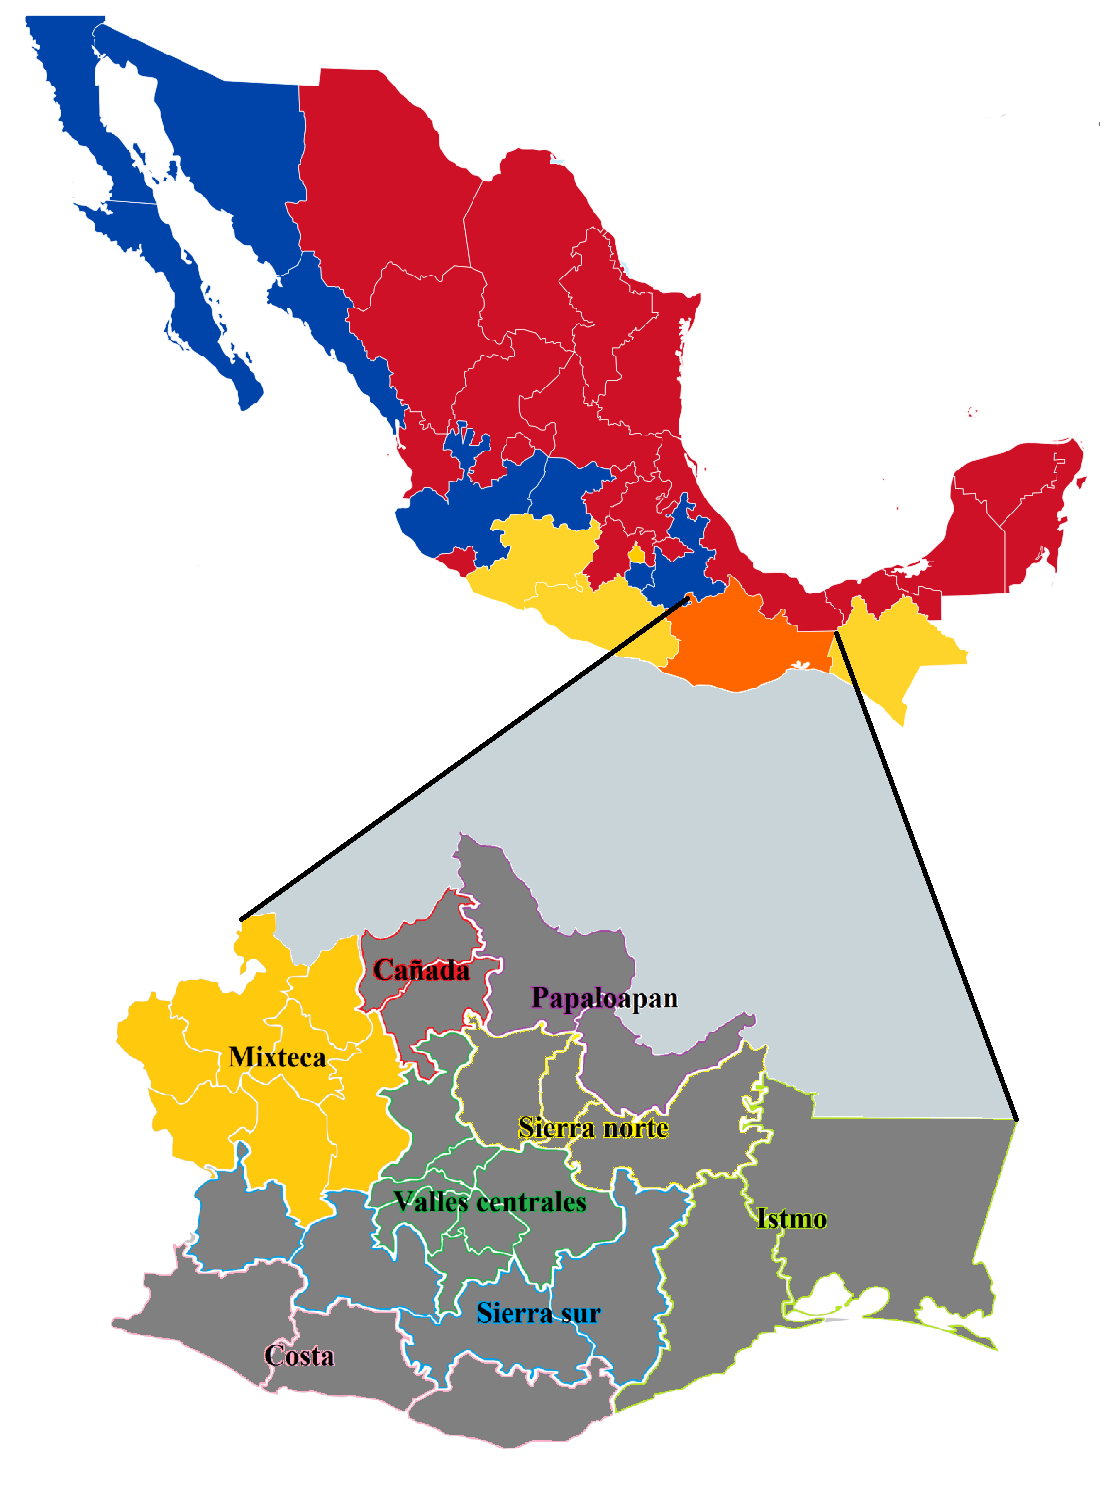
\includegraphics[width=.6\textwidth]{img/macrolocalizacion.png} 
    \caption{Plano de macro localización}
\label{fig:macrolocalizacion}
\end{figure}


\newpage


\subsection{Microlocalización}
Nuestra empresa de cabinas climáticas se enfocará en su sede en la Heroica Ciudad de Huajuapan de León, ubicada en la región Mixteca de Oaxaca. Esta ciudad es una opción estratégica por varias razones:

\textbf{Mercado:} Huajuapan de León cuenta con una población significativa y una actividad comercial vibrante, lo que la convierte en el principal mercado consumidor de la Mixteca.

\textbf{Materias Primas:} La ciudad es un punto de acceso clave para la Mixteca, conectada por las carreteras 190 y 125, facilitando la llegada de proveedores y materias primas desde la Ciudad de México y Puebla.

\begin{figure}[H]
    \centering	
    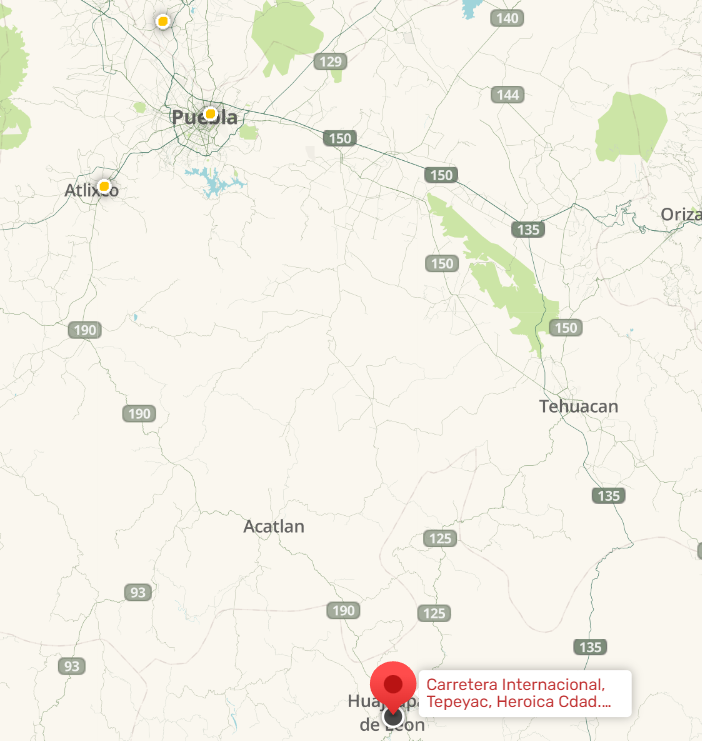
\includegraphics[width=.7\textwidth]{img/carretera190125.png} 
    \caption{Croquis Huajuapan}
\label{fig:croquis190125}
\end{figure}

\textbf{Mano de Obra:} A pesar de la migración, Huajuapan de León atrae a buscadores de empleo debido a su comercio activo, asegurando una oferta de mano de obra disponible para la producción de cabinas climáticas
\newpage

\begin{table}[h!]
\centering
\begin{tabular}{|l|l|}
\hline
\textbf{Infraestructura} & \textbf{Descripción} \\
\hline
Vías de Acceso & Carretera 190 y 125 (ver figura \ref{fig:croquis190125}) \\
\hline
Transporte Urbano & Servicios de autobuses y taxis \\
\hline
Abastecimiento de Agua & 78.3\% de las viviendas con acceso a agua entubada \\
\hline
Manejo de Residuos & Servicios de recolección de basura \\
\hline
Educación & Escuelas primarias, secundarias y universidades \\
\hline
Salud & Hospitales y clínicas locales \\
\hline
\end{tabular}
\caption{Infraestructura disponible en la ciudad de Huajuapan de León (Información Actualizada)}
\label{table:infrahuajuapan}
\end{table}

Como puede verse en la tabla \ref{table:infrahuajuapan}, la ciudad de Huajuapan de León cuenta con la infraestructura necesaria para la construcción de la empresa, destacando el acceso a internet de alta velocidad que recientemente se agregó en la ciudad, también cuenta con la Universidad Tecnológica de la Mixteca que ofrecería el acceso a un personal mejor capacitado. 

\subsection{Aspectos demográficos y económicos}
La región de Huajuapan de León, ubicada en el estado de Oaxaca, latitud: 17°48,28. N 
y longitud: 97°46,46. O, presenta características demográficas y económicas particulares que la hacen un lugar estratégico para el desarrollo de nuestro proyecto de cabinas climáticas para plantas.

Al norte colinda con el estado de Puebla y los municipios de Zapotitlán Palmas, Santiago Miltepec y Asunción Cuyotepeji, al este con los municipios de Asunción Cuyotepeji, Santa María Camotlán, Santiago Huajolotitlán y Santiago Cacaloxtepec, al sur con los municipios de Santiago Cacaloxtepec y San Marcos Arteaga, al oeste con los municipios San Marcos Arteaga, San Jerónimo Silacayoapilla, San Miguel Amatitlán, Santiago Ayuquililla, Zapotitlán Palmas y el estado de Puebla

En términos demográficos, Huajuapan de León ha experimentado un crecimiento poblacional significativo en los últimos años. Según el último censo, la población en 2020 fue de 78,313 habitantes, lo que representa un crecimiento del 12.1\% \cite{PoblacionHuajuapan2020} en comparación con 2010. de la población total, el 47.5\% son hombres y el 52.5\% son mujeres

En cuanto a la economía, la Inversión Extranjera Directa (IED) en Oaxaca alcanzó los US\$43.9M en el periodo de enero a diciembre de 2023, lo que indica un ambiente favorable para el desarrollo de proyectos empresariales.

Además, la tasa de desempleo en Oaxaca en el cuarto trimestre de 2023 fue del 1.54\%, lo que sugiere la disponibilidad de mano de obra en la región. Sin embargo, es importante destacar que la tasa de informalidad laboral alcanzó el 81.1\% \cite{DataMexicoHuajuapan2023}, lo que representa un desafío en términos de equidad laboral.

Estos aspectos demográficos y económicos son fundamentales para entender el entorno en el que se desarrollará nuestro proyecto y para diseñar estrategias que permitan maximizar su impacto en la región.

\subsection{Croquis de localización}
Nuestra área de interés dentro de la ciudad de Huajuapan de León es en un lugar cerca del centro pero a su vez que esté en las orillas, es por eso que se decidió usar las antiguas instalaciones del grupo PEPSICO, ya que está a un costado de la carretera 190 y además ya cuenta con la mayoría de la infraestructura realizada, por lo que solamente se reacondicionaría el lugar y construir las áreas faltantes. 

Se ubica en la colonia el Tepeyac, Juan Diego \#19, esquina con Díaz Ordaz.

\begin{figure}[H]
    \centering	
    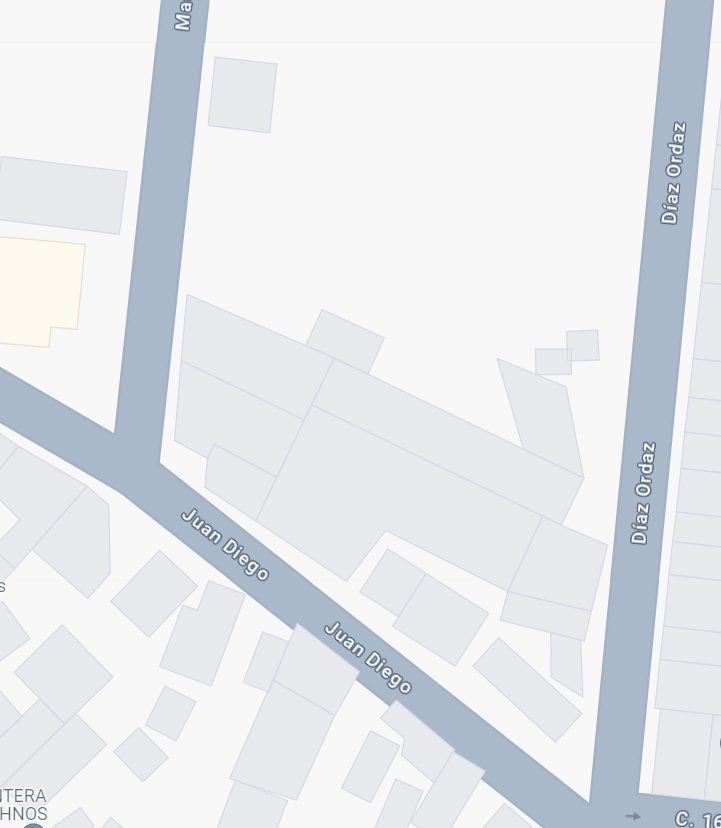
\includegraphics[width=.7\textwidth]{img/Empresa/ubicacion1.png} 
    \caption{Croquis de la localización de la empresa}
\label{fig:croquis1}
\end{figure}

\begin{figure}[H]
    \centering	
    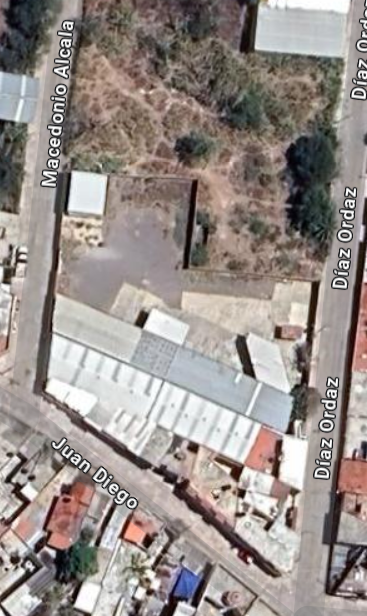
\includegraphics[width=.7\textwidth]{img/Empresa/ubicacion2.png} 
    \caption{Croquis satelital de la localización de la empresa}
\label{fig:croquis1}
\end{figure}

\newpage

\section{Capacidad óptima de producción}

La capacidad de producción es el volumen máximo de productos que puede generar una planta o empresa de manufactura en un período determinado, utilizando los recursos disponibles. Es crucial para calcular el rendimiento financiero futuro y establecer una línea de tiempo confiable para la entrega de los productos.

   \begin{itemize}
       \item Se llevó a cabo un estudio exhaustivo del mercado de cabinas para el cuidado de plantas, incluyendo la revisión de informes de la industria, análisis de tendencias de consumo y entrevistas con expertos del sector.
       \item Se recopiló información sobre la demanda actual y proyectada de cabinas para el cuidado de plantas, considerando factores demográficos, hábitos de consumo y tendencias de estilo de vida.
       \item Se identificaron segmentos de mercado clave, como propietarios de viviendas, entusiastas de la jardinería, restaurantes y hoteles, para comprender sus necesidades y preferencias.
   \end{itemize}

\subsection{Capacidad de producción actual}


La empresa \textbf{“Terra Green”} se especializa en la fabricación de cabinas diseñadas para el cuidado óptimo de plantas en entornos controlados. Según los datos recabados en la proyección de la demanda (página 8), se estima una demanda de \textbf{280,000 unidades en el primer año}. Sin embargo, Terra Green ha decidido satisfacer solo el \textbf{5 por ciento de esa demanda}, lo que implica producir \textbf{14,000 unidades al año} o \textbf{1,167 unidades al mes}.

Para diseñar un sistema de producción con un máximo de \textbf{3 por ciento de error}, se espera una producción de \textbf{1,203 unidades al mes}, lo que se traduce en \textbf{300 unidades por semana} o \textbf{60 unidades al día}.

\textbf{Parámetros de Producción:}
\begin{itemize}
    \item \textbf{Jornada Laboral:} Se propone una jornada de 16 horas (dos turnos) sin cargo extra según CFE.
    \item \textbf{Capacidad de Producción por Hora:} Se espera que cada hora se produzcan 3.75 unidades.
    \item \textbf{Tiempo de Producción por Pieza:} El tiempo de producción total por cada pieza es de 16 minutos, siendo esta la máxima capacidad de producción.
\end{itemize}

\textbf{Diseño y Características de las Cabinas:}
\begin{itemize}
    \item \textbf{Espacio Interior:} Las cabinas se diseñarán en diferentes tamaños para acomodar una variedad de plantas, desde pequeñas hierbas hasta árboles frutales en macetas. Se utilizarán materiales transparentes (vidrio o plástico) para permitir la entrada de luz natural y la observación de las plantas.
    \item \textbf{Sistemas de Control Ambiental:} Se incorporarán sensores de temperatura, humedad y luz para monitorear y ajustar automáticamente las condiciones internas. Los sistemas de riego automático y ventilación serán parte integral del diseño.
    \item \textbf{Materiales y Construcción:} Las cabinas se construirán con paneles aislantes para mantener una temperatura constante. Se utilizarán materiales reciclables y sostenibles siempre que sea posible.
    \item \textbf{Eficiencia Energética:} Se implementarán luces LED de bajo consumo energético para la iluminación interna. El sistema de calefacción y refrigeración se optimizará para minimizar el gasto energético.
\end{itemize}

\textbf{Beneficios para los Clientes:}
\begin{itemize}
    \item Las cabinas de Terra Green ofrecerán un entorno ideal para el crecimiento de plantas en interiores.
    \item Los usuarios podrán cultivar hierbas, flores y vegetales durante todo el año, independientemente del clima exterior.
    \item La durabilidad y eficiencia energética garantizarán una inversión a largo plazo.
\end{itemize}




  

\section{Ingeniería del proyecto}

\subsection{Proceso de Producción}

\begin{itemize}
    \item \textbf{Diseño y Planificación:}
    \begin{itemize}
        \item El equipo de diseño de Terra Green crea los planos y especificaciones detalladas para las cabinas. Esto incluye el tamaño, la disposición interna, los materiales y los sistemas de control ambiental.
        \item Se definen los parámetros clave, como la capacidad de producción, el tiempo de producción por pieza y la jornada laboral.
    \end{itemize}
    
    \item \textbf{Adquisición de Materiales:}
    \begin{itemize}
        \item Se adquieren los materiales necesarios para la construcción de las cabinas. Esto puede incluir paneles de vidrio o plástico transparente, aislantes, sensores, luces LED y otros componentes.
    \end{itemize}
    
    \item \textbf{Fabricación de Componentes:}
    \begin{itemize}
        \item Se fabrican los componentes básicos de las cabinas, como los paneles laterales, las puertas, los estantes y los sistemas de iluminación.
        \item Los sistemas de control ambiental (sensores, sistemas de riego, ventilación) también se ensamblan y prueban.
    \end{itemize}
    
    \item \textbf{Ensamblaje de las Cabinas:}
    \begin{itemize}
        \item Se ensamblan las cabinas siguiendo los planos de diseño. Se unen los paneles, se instalan las puertas y se conectan los sistemas de control.
        \item Se aplican los acabados exteriores y se asegura la estabilidad y durabilidad de cada cabina.
    \end{itemize}
    
    \item \textbf{Control de Calidad:}
    \begin{itemize}
        \item Cada cabina pasa por un riguroso control de calidad. Se verifica que todos los componentes funcionen correctamente y que las condiciones internas sean las adecuadas.
        \item Se realizan pruebas de resistencia, eficiencia energética y seguridad.
    \end{itemize}
    
    \item \textbf{Embalaje y Almacenamiento:}
    \begin{itemize}
        \item Las cabinas se embalan cuidadosamente para su transporte. Se protegen contra daños durante el envío.
        \item Se almacenan en el área de distribución hasta su entrega a los clientes.
    \end{itemize}
    
    \item \textbf{Entrega y Montaje:}
    \begin{itemize}
        \item Las cabinas se entregan a los clientes según sus pedidos. El equipo de instalación de Terra Green se encarga del montaje en el lugar deseado.
        \item Se realizan pruebas finales para asegurar que todo funcione correctamente.
    \end{itemize}
    
    \item \textbf{Servicio Postventa:}
    \begin{itemize}
        \item Terra Green ofrece soporte técnico y mantenimiento a sus clientes. Cualquier problema o ajuste necesario se atiende de manera rápida y eficiente.
    \end{itemize}
\end{itemize}

\subsection{Distribución de planta}

El proyecto de la empresa constructora de cabinas para el cuidado de plantas en México es de gran envergadura, considerando la creciente demanda de soluciones de jardinería urbana y el interés cada vez mayor en el cultivo de plantas en interiores.

Para satisfacer esta demanda, la empresa planea establecer una planta de producción de tamaño considerable en una ubicación estratégica, que permita el acceso fácil a materias primas y mano de obra calificada, así como una logística eficiente para la distribución de los productos terminados.

Además, se contempla la posibilidad de ampliar las instalaciones en el futuro para aumentar la capacidad de producción y diversificar la oferta de productos, incluyendo diferentes tamaños y diseños de cabinas para satisfacer las necesidades de diversos segmentos de mercado.


La distribución de la planta de producción se ha diseñado cuidadosamente para optimizar el flujo de materiales y minimizar los tiempos muertos en el proceso de fabricación.

En primer lugar, se han establecido áreas dedicadas para cada etapa del proceso de producción, desde el almacenamiento de materias primas hasta el ensamblaje final y las pruebas de calidad. Esto permite una organización eficiente del trabajo y facilita la supervisión y el control de cada fase del proceso.

Además, se han implementado sistemas de transporte interno, como cintas transportadoras y carretillas elevadoras, para facilitar el movimiento de materiales entre las diferentes áreas de la planta. Esto reduce el tiempo de manipulación de materiales y aumenta la productividad general de la planta.

Por último, se han instalado equipos de seguridad y medidas de prevención de accidentes en toda la planta para garantizar un entorno de trabajo seguro y cumplir con las regulaciones laborales vigentes en México



\begin{table}[H]
    \centering
    \caption{Actividades, Descripción y Equipo Necesario para la Producción de Cabinas}
    \begin{tabular}{|l|p{0.4\textwidth}|p{0.4\textwidth}|}
        \hline
        \textbf{Actividad} & \textbf{Descripción de la Actividad} & \textbf{Equipo Necesario} \\
        \hline
        Diseño y Planificación & Creación de planos y especificaciones detalladas para la cabina. Incluye tamaño, disposición interna y sistemas de control ambiental. & Equipo de diseño, software de diseño asistido por computadora (CAD). \\
        \hline
        Adquisición de Materiales & Compra de materiales necesarios para la construcción de la cabina. Incluye paneles de vidrio o plástico transparente, aislantes, sensores, luces LED, etc. & Departamento de compras, proveedores. \\
        \hline
        Fabricación de Componentes & Producción de partes básicas de la cabina, como paneles laterales, puertas, estantes y sistemas de iluminación. & Máquinas de corte, soldadoras, herramientas manuales. \\
        \hline
        Ensamblaje de las Cabinas & Montaje de la cabina siguiendo los planos de diseño. Unión de paneles, instalación de puertas y conexión de sistemas de control. & Herramientas de ensamblaje, personal de producción. \\
        \hline
        Control de Calidad & Verificación de que todos los componentes funcionen correctamente y que las condiciones internas sean adecuadas. Pruebas de resistencia, eficiencia energética y seguridad. & Personal de calidad, equipos de prueba. \\
        \hline
        Embalaje y Almacenamiento & Empaque cuidadoso de la cabina para transporte. Protección contra daños durante el envío. Almacenamiento en área de distribución. & Materiales de embalaje, área de almacenamiento. \\
        \hline
        Entrega y Montaje & Entrega de la cabina al cliente según pedido. Montaje en el lugar deseado por el equipo de instalación. & Personal de entrega, herramientas de montaje. \\
        \hline
        Servicio Postventa & Soporte técnico y mantenimiento para los clientes. Atención rápida y eficiente a problemas o ajustes. & Personal de servicio al cliente, herramientas de reparación. \\
        \hline
    \end{tabular}
\end{table}


\section*{Planta Arquitectónica del Proyecto}

\subsection*{\textbf{Descripción por Área}}

\begin{itemize}
    \item \textbf{Recepción de Materiales:}
    \begin{itemize}
        \item \textbf{Dimensión:} 150 m\textsuperscript{2}
        \item \textbf{Ubicación:} En la entrada principal de la planta.
        \item \textbf{Conexiones:} Con el área de corte de materiales y el área de almacenamiento.
    \end{itemize}

    \item \textbf{Corte de Materiales:}
    \begin{itemize}
        \item \textbf{Dimensión:} 960 m\textsuperscript{2}
        \item \textbf{Ubicación:} Adyacente a la recepción de materiales.
        \item \textbf{Conexiones:} Con el área de montaje de estructuras y el área de instalación de sistemas.
    \end{itemize}

    \item \textbf{Montaje de Estructura:}
    \begin{itemize}
        \item \textbf{Dimensión:} 2000 m\textsuperscript{2}
        \item \textbf{Ubicación:} Contigua al área de corte de materiales.
        \item \textbf{Conexiones:} Con el área de pruebas de calidad y el área de empacado y almacenamiento.
    \end{itemize}

    \item \textbf{Instalación de Sistemas:}
    \begin{itemize}
        \item \textbf{Dimensión:} 1280 m\textsuperscript{2}
        \item \textbf{Ubicación:} Junto al área de corte de materiales.
        \item \textbf{Conexiones:} Con el área de montaje de estructuras y el área de pruebas de calidad.
    \end{itemize}

    \item \textbf{Pruebas de Calidad:}
    \begin{itemize}
        \item \textbf{Dimensión:} 400 m\textsuperscript{2}
        \item \textbf{Ubicación:} Al lado del área de montaje de estructuras.
        \item \textbf{Conexiones:} Con el área de instalación de sistemas y el área de empacado y almacenamiento.
    \end{itemize}

    \item \textbf{Empaque y Almacenamiento:}
    \begin{itemize}
        \item \textbf{Dimensión:} 400 m\textsuperscript{2}
        \item \textbf{Ubicación:} Adyacente al área de pruebas de calidad.
        \item \textbf{Conexiones:} Con el área de montaje de estructuras y el área de corte de materiales.
    \end{itemize}

    \item \textbf{Estacionamiento para Empleados:}
    \begin{itemize}
        \item \textbf{Dimensión:} 500 m\textsuperscript{2}
        \item \textbf{Ubicación:} Junto a la entrada principal de la planta.
    \end{itemize}

    \item \textbf{Oficinas Administrativas:}
    \begin{itemize}
        \item \textbf{Dimensión:} 600 m\textsuperscript{2}
        \item \textbf{Ubicación:} En un área central de la planta.
    \end{itemize}

    \item \textbf{Área de Descanso:}
    \begin{itemize}
        \item \textbf{Dimensión:} 200 m\textsuperscript{2}
        \item \textbf{Ubicación:} Cerca de las oficinas administrativas.
    \end{itemize}
\end{itemize}

\subsection*{\textbf{Dimensión Total de la Planta:} 6690 m\textsuperscript{2}}




\newpage

\section{Inversión fija}




\begin{figure}[H]
    \centering	
    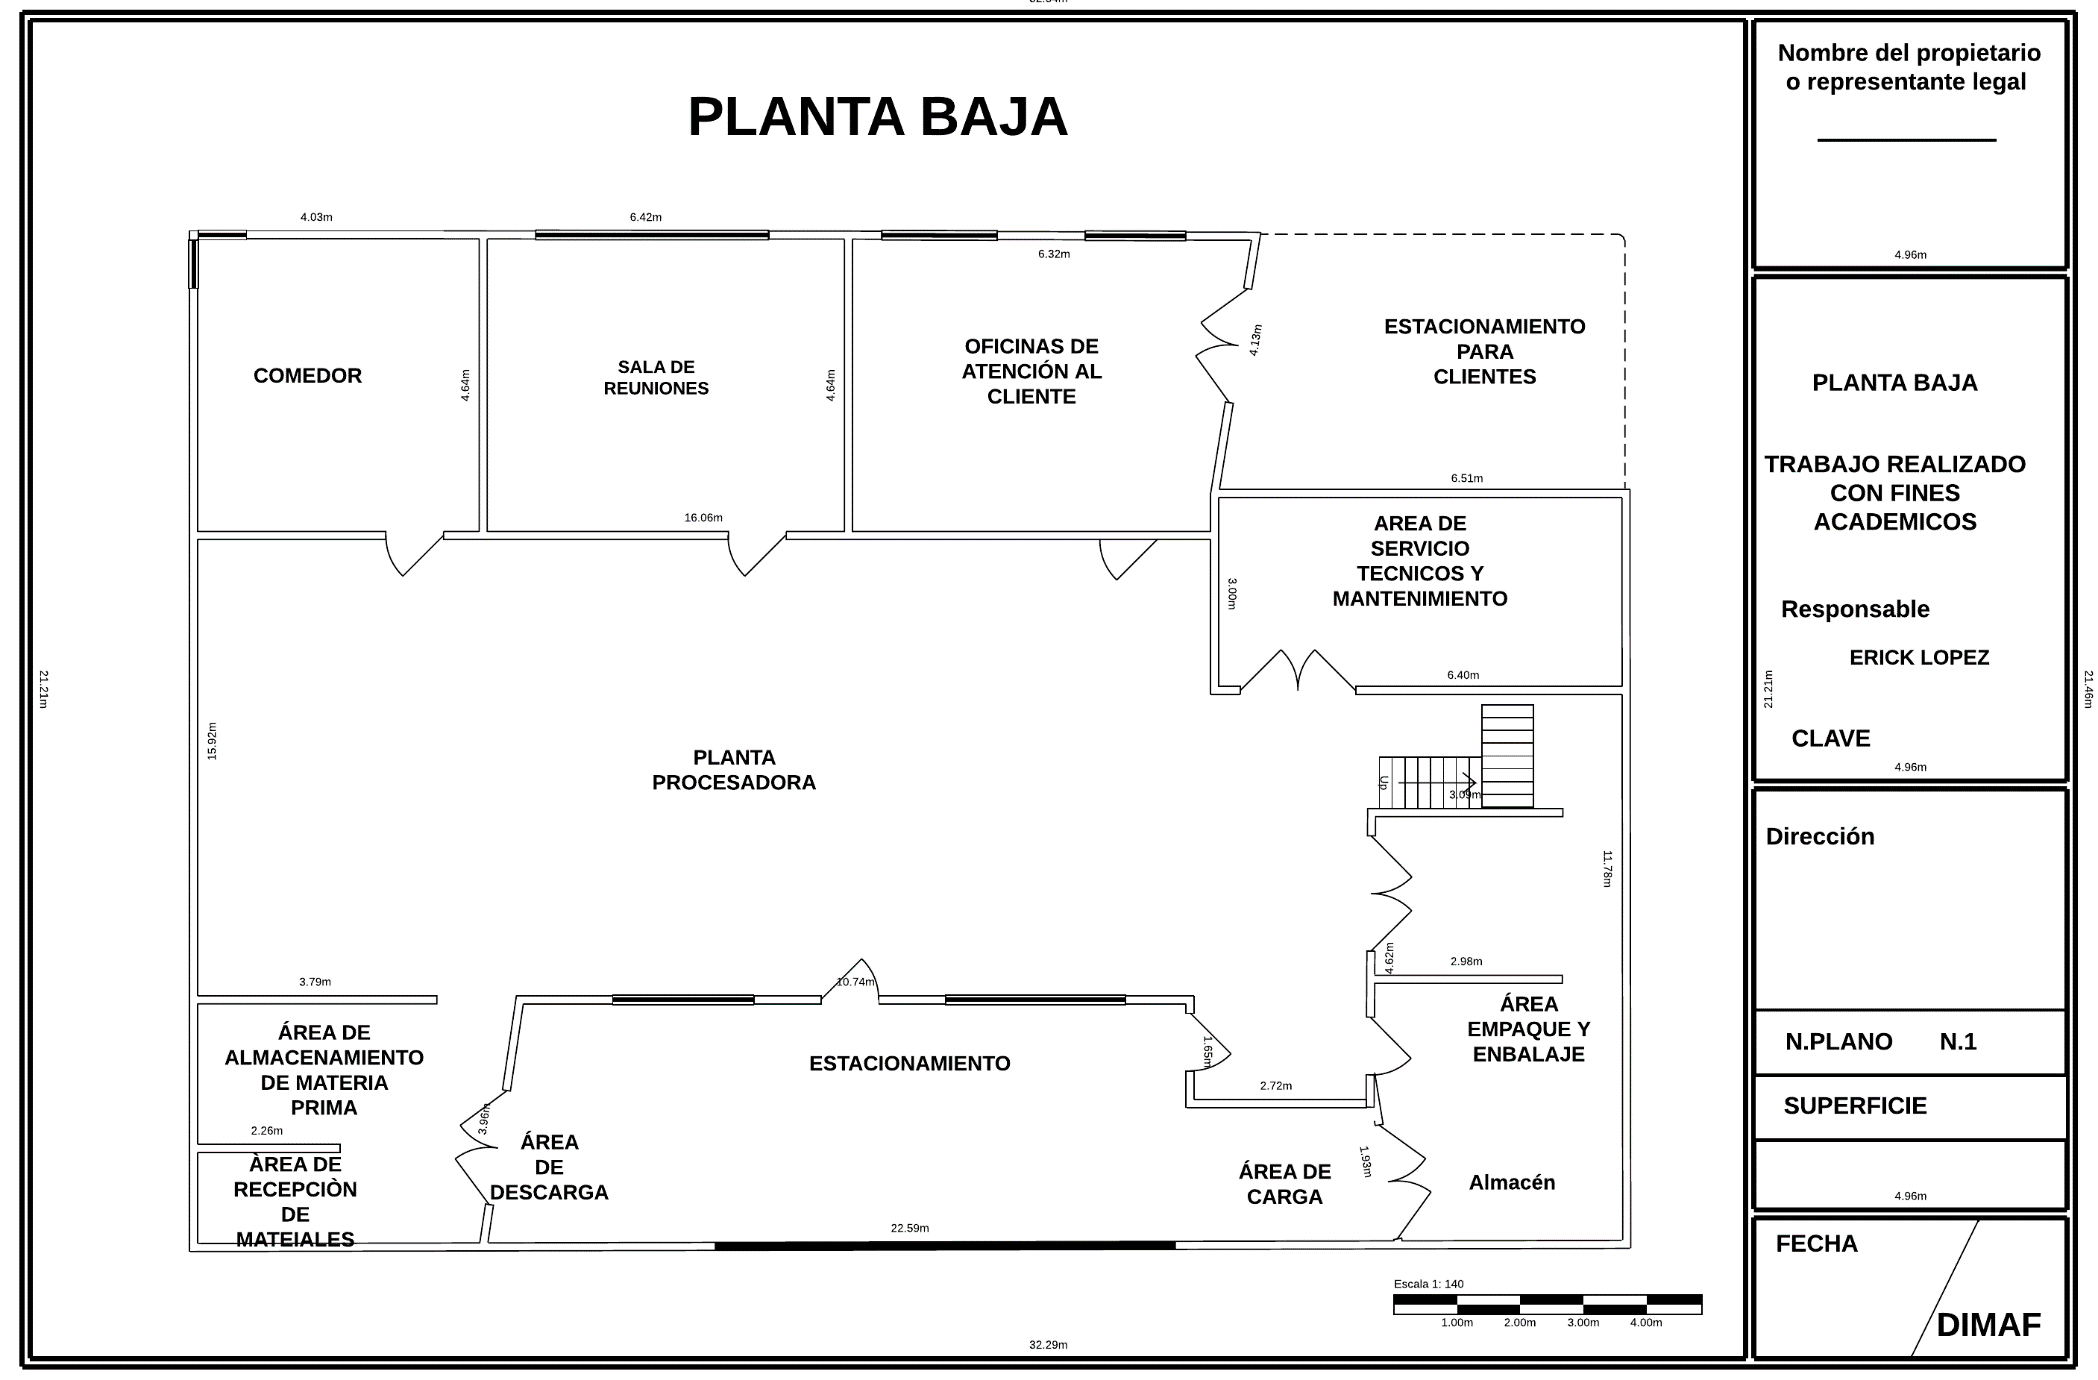
\includegraphics[angle=90,width=1.0\textwidth]{chapters/image1_.png} 
    \caption{Planta baja}
\label{fig:croquis190125}
\end{figure}

\begin{figure}[H]
    \centering	
    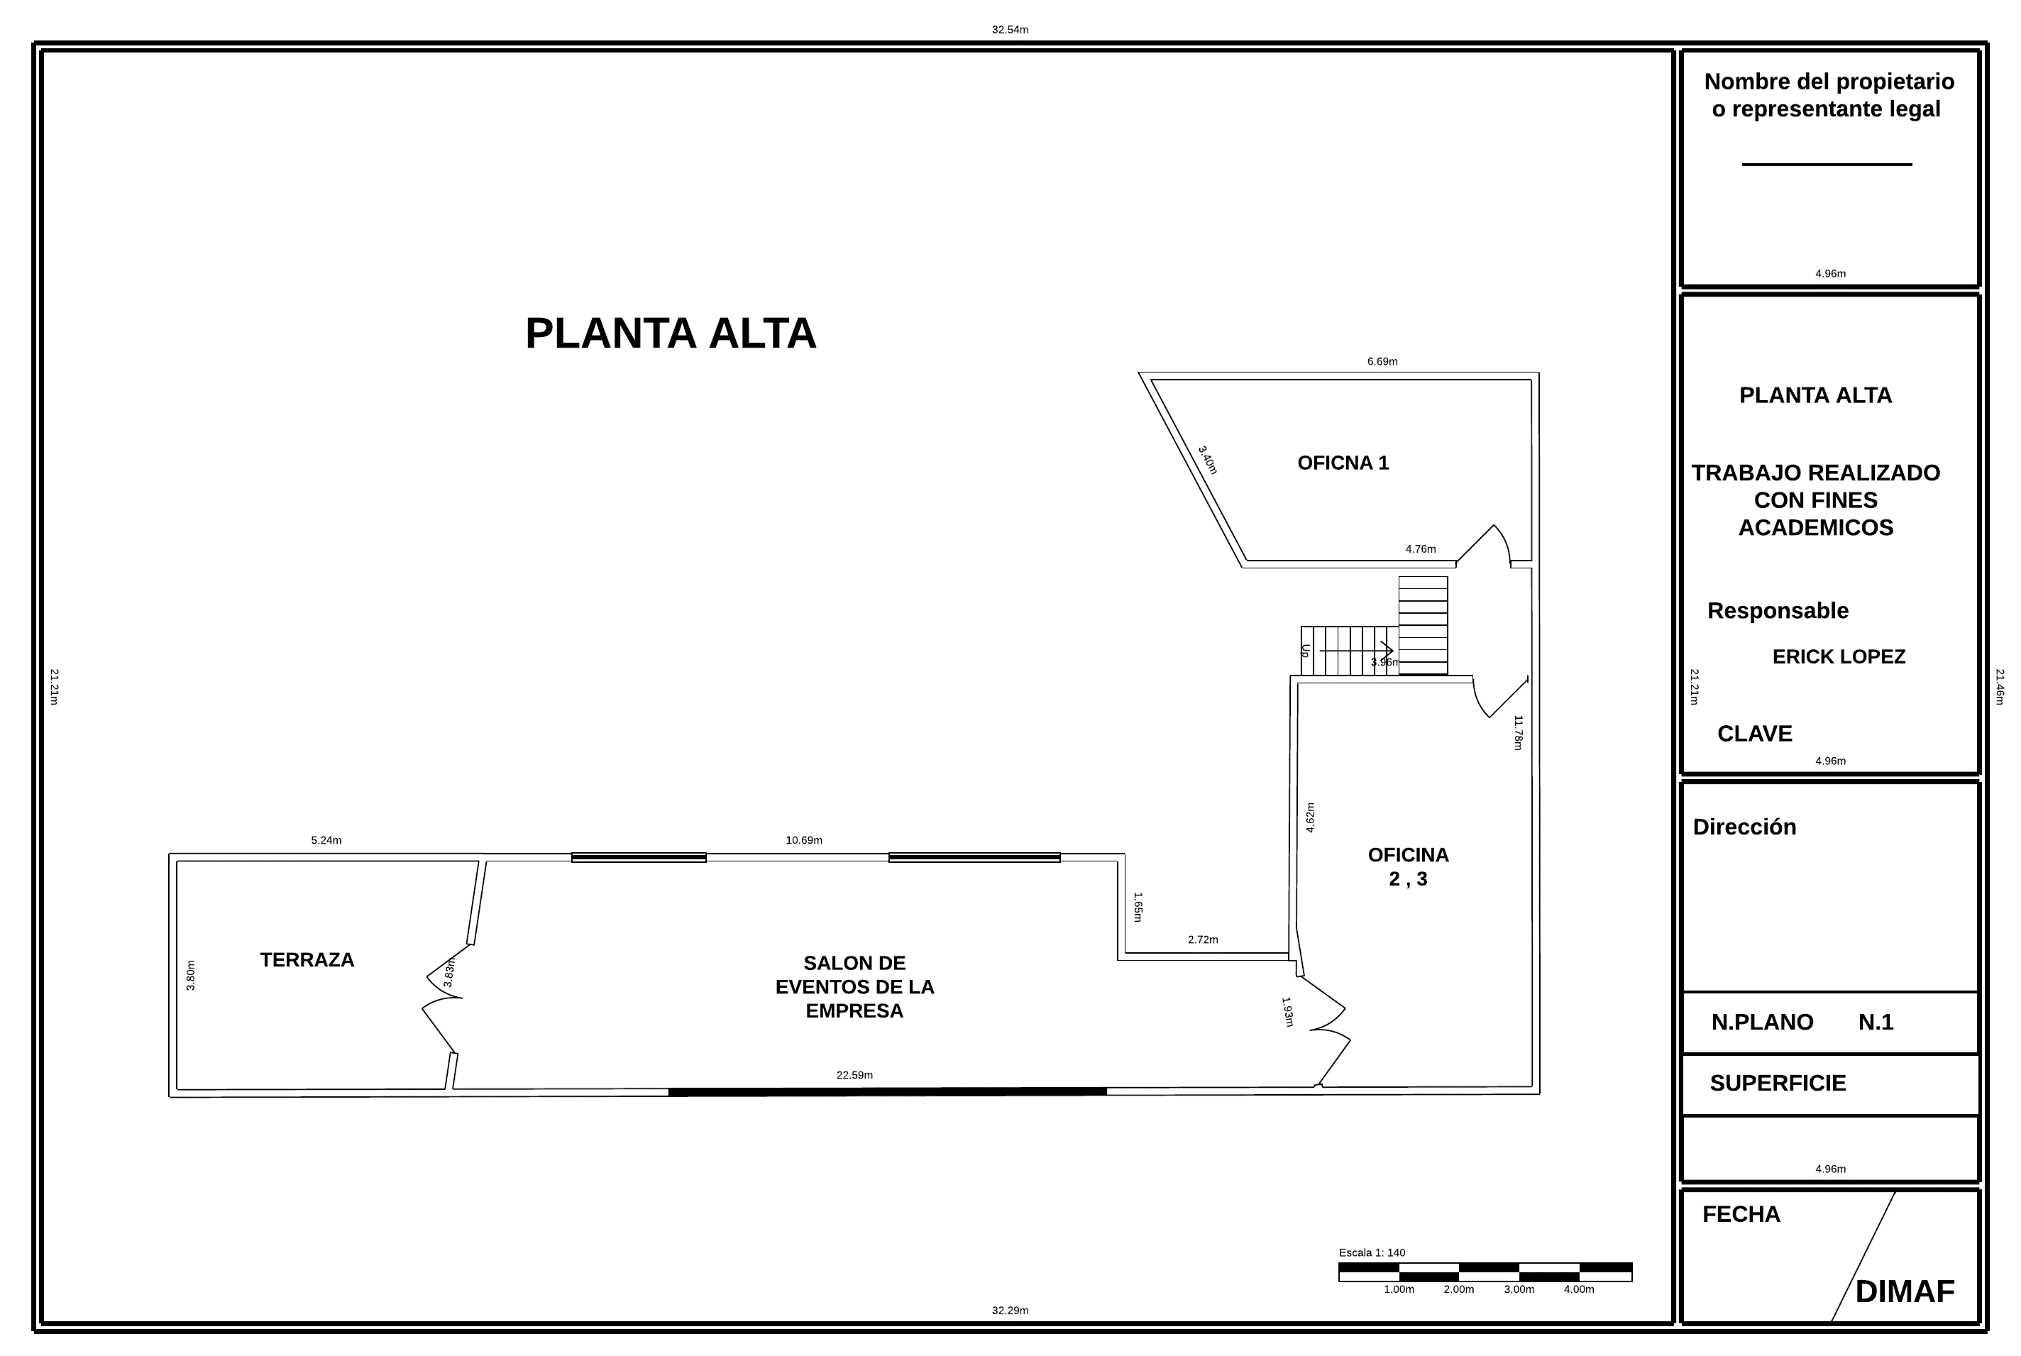
\includegraphics[angle=90,width=1.0\textwidth]{chapters/image2_.png} 
    \caption{Planta alta}
\label{fig:croquis190125}
\end{figure}

\begin{figure}[H]
    \centering	
    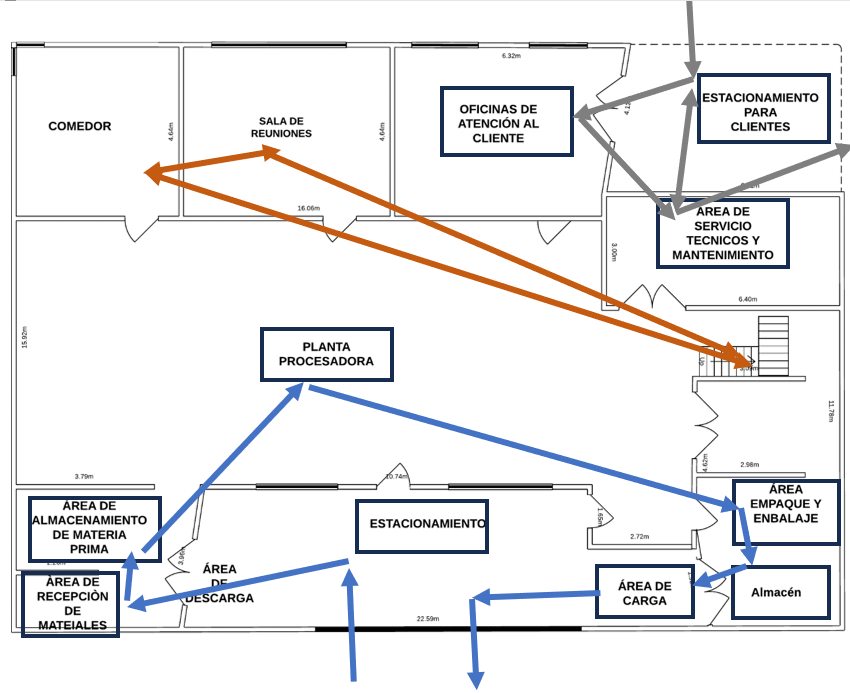
\includegraphics[angle=90,width=0.75\textwidth]{chapters/ELC_HILOS.png} 
    \caption{Diagrama de hilos}
\label{fig:croquis190125}
\end{figure}

Se tienen 3 principales hilos los cuales comprenden a 

1. Color gris

Es cuando una persona externa visita la empresa y esta desea un servicio técnico, atención a cliente o un acercamiento más a la empresa.

2. Color naranja

Área que recorre el personal administrativo y estos se conectan directamente a la segunda planta con las demás áreas administrativas.

3. Color azul 

Es la ruta que toman la contracción del producto desde recepción de materia prima hasta la entrega el producto final este camino es unidireccional, ya que no se puede regresar el material a un estado anterior. 

\begin{figure}[H]
    \centering	
    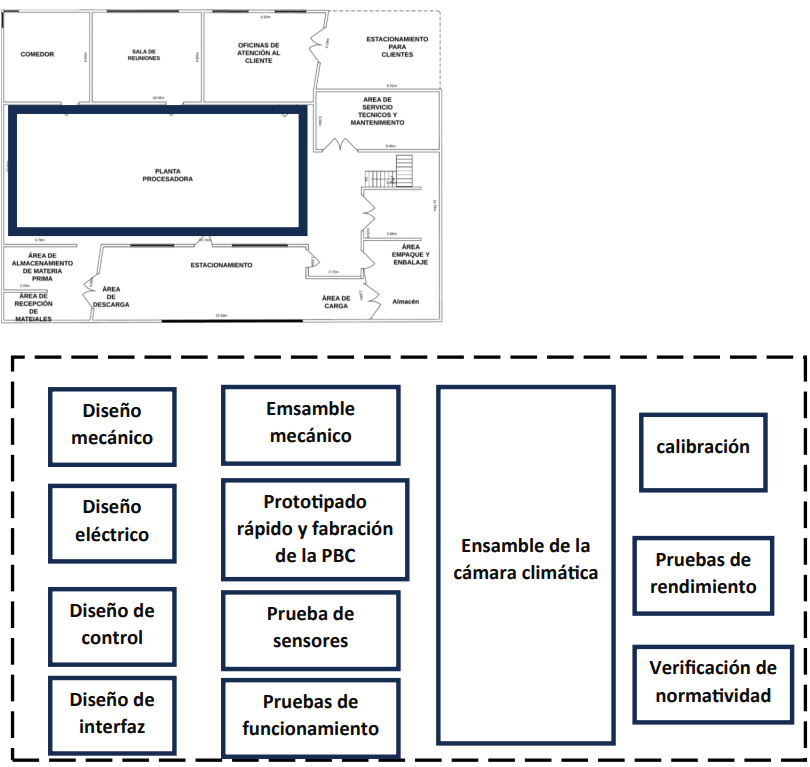
\includegraphics[angle=0,width=0.67\textwidth]{chapters/ELC_DIAGRAM.png} 
    \caption{Diagrama de distribución del área de producción}
\label{fig:croquis190125}
\end{figure}

Para poder producir las cámaras climáticas en necesario tener una distribución uniforme y las áreas no deben de estar alejadas, ya que nos reduce el tiempo de movimiento de materiales además de poder interactuar con las demás área para un correcto flujo y detección de errores.

\begin{figure}[H]
    \centering	
    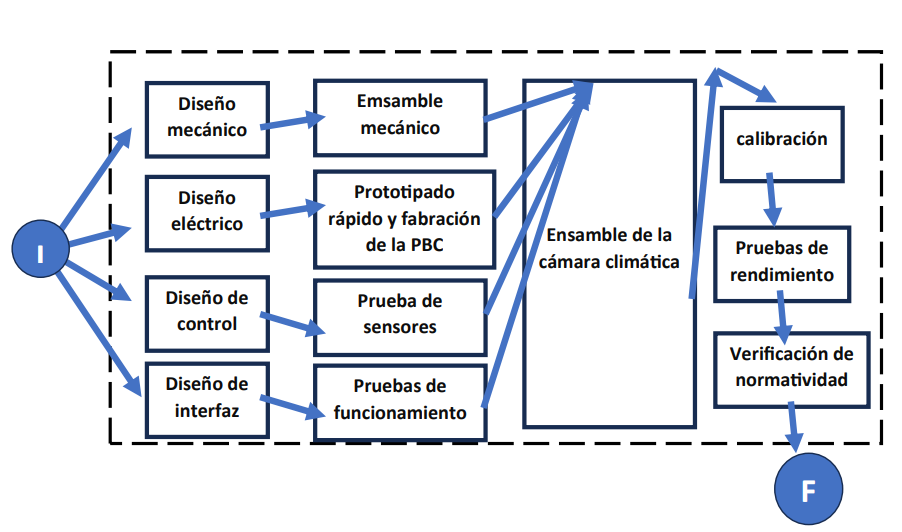
\includegraphics[angle=0,width=0.70\textwidth]{chapters/ELC_DIAGRAM2.png} 
    \caption{Diagrama hilos de la distribución del área de producción}
\label{fig:croquis190125}
\end{figure}

Se diseñó el área de producción para poder tener 4 áreas en este caso trabajando al mismo tiempo para aumentar efectividad y reducir los tiempos con ello podemos desarrollar productos más rápidos y permitir realizar productos personalizados cuando sea su caso. 
%----------------------------------------





\subsection{Adquisición del equipo de transporte}

Este punto implica la compra de equipos de transporte como transportadores de banda, carretillas elevadoras, o cualquier otro equipo necesario para el movimiento de materias primas, productos semiacabados y productos terminados dentro de la planta.

Se debe considerar la capacidad de carga, la eficiencia energética y la seguridad de estos equipos al seleccionarlos.

La inversión en equipos de transporte adecuados es crucial para garantizar un flujo de trabajo eficiente y minimizar los tiempos de inactividad en la planta.

\begin{table}[htbp]
    \centering
    \begin{tabular}{|l|c|c|c|}
        \hline
        \textbf{Concepto}               & \textbf{Cantidad} & \textbf{Costo Unitario} & \textbf{Importe} \\
        \hline
        Transportador de banda          & 2                 & \$10,000.00              & \$20,000.00      \\
        Carretilla elevadora eléctrica & 1                 & \$15,000.00              & \$15,000.00      \\
        Plataforma móvil                & 1                 & \$8,000.00               & \$8,000.00       \\
        \hline
        Subtotal                        &                   &                          & \$43,000.00      \\

        IVA (16\%)                      &                   &                          & \$6,880.00       \\
        \hline
        TOTAL                           &                   &                          & \$49,880.00      \\
        \hline
    \end{tabular}
    \caption{Adquisición de Equipo de Transporte}
    \label{tab:equipo_transporte}
\end{table}

Se considera la adquisición de una plataforma móvil que puede ser útil para tareas de mantenimiento o para acceder a áreas elevadas dentro de la planta.

El subtotal muestra el costo total de todos los elementos de equipo de transporte, mientras que el IVA representa el impuesto sobre el valor agregado aplicable. El total general refleja el costo total, incluido el impuesto.

\subsection{Adquisición de herramientas y refacciones}

Este punto implica la compra de herramientas específicas necesarias para el mantenimiento y la reparación de equipos, así como para llevar a cabo tareas operativas diarias.
Además de las herramientas, la adquisición de refacciones es esencial para garantizar la disponibilidad de piezas de repuesto para equipos críticos y minimizar el tiempo de inactividad en caso de averías.

\begin{table}[htbp]
    \centering
    \begin{tabular}{|l|c|c|c|}
        \hline
        \textbf{Concepto}               & \textbf{Cantidad} & \textbf{Costo Unitario} & \textbf{Importe} \\
        \hline
        Juego de llaves métricas       & 3 juegos          & \$200.00                 & \$600.00         \\
        Juego de destornilladores      & 3 juegos          & \$150.00                 & \$450.00         \\
        Equipo de soldadura            & 1                 & \$1,000.00               & \$1,000.00       \\
        Equipo de medición             & 1                 & \$800.00                 & \$800.00         \\
        Piezas de repuesto    & Varios            & \$500.00                 & \$2,000.00       \\
        \hline
        Subtotal                       &                   &                          & \$4,850.00       \\
        IVA (16\%)                     &                   &                          & \$776.00         \\
        \hline
        TOTAL                          &                   &                          & \$5,626.00       \\
        \hline
    \end{tabular}
    \caption{Adquisición de Herramientas y Refacciones}
    \label{tab:herramientas_refacciones}
\end{table}

El equipo de soldadura es necesario para realizar reparaciones en caso de daños en componentes metálicos, mientras que el equipo de medición es esencial para garantizar la precisión en la instalación y ajuste de equipos.

Tambien se considera la compra de piezas de repuesto, lo que garantiza la disponibilidad de repuestos en caso de averías o fallos en los componentes críticos para el sistema de control de planta.




\section{Sistema de producción}
\subsection{Requerimientos técnicos del producto}

Entre los principales requerimientos del producto están:

\begin{itemize}
    \item Dimensiones de 0.5mx0.5mx0.8m
    \item Respetar la norma NOM 059 SEMARNAT-2010.
    \item El contenedor se construirá con material que brinde seguridad tanto a la planta como al usuario.
\end{itemize}

\subsubsection{Materias primas primarias.}

En la anterior sección \textbf{Análisis de la materia prima (pg. 3)} se nombran algunos materiales esenciales en la elaboración del producto, sin embargo aquí se enlistan las primarias.

\begin{itemize}
    \item Madera
    \item Acrílico
    \item Tornillos
    \item Adhesivo
\end{itemize}

\subsubsection{Materiales indirectos}

\begin{itemize}
    \item \textbf{Envases primarios:} Se planea entregar el producto final ensamblado aunque esto signifique una mayor demanda de transporte. El transporte llevará el producto final empaquetado en una caja de madera rellena de un material que evite daños al momento de ser transportada.
    \item \textbf{Envases secundarios:} Al momento del transporte, se pueden estibar un máximo de unidades y se pude hacer uso de tiras de plástico para hacer la estructura más estable.
\end{itemize}



\begin{figure}[H]
    \centering	
    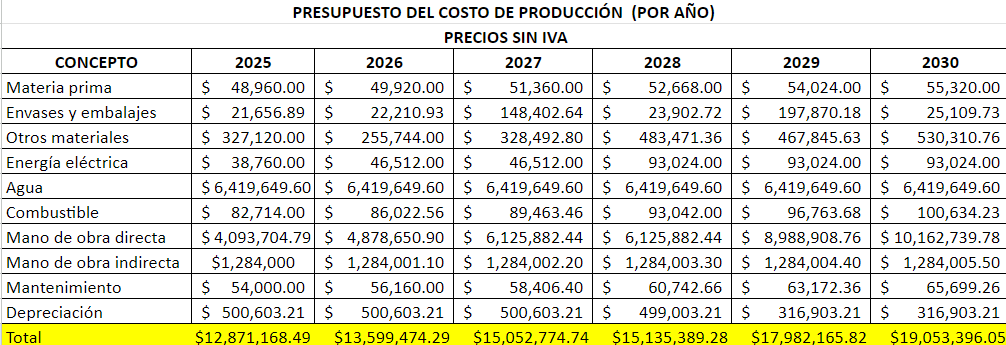
\includegraphics[angle=0,width=0.9\textwidth]{chapters/ELC_Produccion.png} 
    \caption{Costo de producción por año}
\label{fig:croquis190125}
\end{figure}



\subsection{Costo unitario}

Como se estimó en la sección \textbf{Análisis de precio (pg. 12)}, se toman en cuenta los datos de varios modelos disponibes en plataformas de comercio internacional y se cuenta con un precio aproximado de \$6,000, sin embargo, el producto ofrece más funciones con los que no cuenta la competencia, así que se puede establecer un precio de aproximadamente \$8,000, teniendo un margen de ganancia de \$2,500 por producto

\begin{figure}[H]
    \centering	
    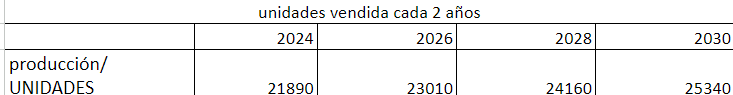
\includegraphics[angle=0,width=0.9\textwidth]{chapters/ELC_Unidades+.png} 
    \caption{Unidades de producción cada dos años}
\label{fig:croquis190125}
\end{figure}

\newpage



\newpage

\section{Conclusiones del estudio técnico}

Con el estudio técnico se encontró la tecnología adecuada para aplicar al desarrollo de las cámaras climáticas así como la evaluación de la disponibilidad de componentes en el mercado par asegurar una cadena de suministro estable, se evaluó el costo de producción por año como el de una unidad para poder comparar los pecios contra el mercado. Para poder operar de manera fácil y poder acceder a los usuarios finales se realizó la evaluación para la ubicación de la empresa. Ahora para poder tener el espacio suficiente y una adecuada distribución se optó por el desarrollo de la planta. Para poder iniciar a producir se requerirá tecnología de producción a lo cual se analizó el costo de la maquinaria así como de las diferentes áreas técnicas y administrativas.
\chapter{Estudio Administrativo Legal}

\section{Filosofía de la empresa}

\subsection{Misión}


Ofrecer soluciones innovadoras y sostenibles para el cultivo de plantas en entornos controlados. Nos especializamos en el diseño y fabricación de cabinas de alta calidad que optimizan el cuidado de las plantas al proporcionar condiciones ideales de luz, temperatura y humedad.



\subsection{Visión}

Nos visualizamos como líderes en la industria de cabinas para el cuidado de plantas, contribuyendo tanto al bienestar de las personas como al cuidado del medio ambiente. Ser reconocidos por nuestra excelencia en diseño, tecnología y nuestro firme compromiso con la sustentabilidad.


\subsection{Valores de la empresa}

\begin{itemize}

 \item \textbf{Innovación:} Estamos en busca de nuevas maneras de mejorar nuestras cabinas y procesos.
    \item \textbf{Calidad:} Nos dedicamos a ofrecer productos que sean duraderos y confiables.
    \item \textbf{Sostenibilidad:} Prestamos atención al impacto ambiental en cada etapa de producción.
    \item \textbf{Colaboración:} Trabajamos codo a codo con nuestros clientes y socios para alcanzar resultados excepcionales.

\end{itemize}

\subsection{Politicas de la empresa}


\begin{itemize}
    \item \textbf{Compromiso con la Sostenibilidad:} Nos comprometemos a diseñar y fabricar nuestras cabinas de manera sostenible, utilizando materiales y procesos de producción eficientes. Buscamos reducir nuestra huella de carbono y minimizar el impacto ambiental en cada etapa de la cadena de suministro.
    
    \item \textbf{Calidad y Durabilidad:} Nuestro objetivo es ofrecer productos de alta calidad y duraderos. Todas nuestras cabinas están diseñadas para resistir el paso del tiempo y brindar un servicio confiable a nuestros clientes.
    
    \item \textbf{Atención al Cliente:} Valoramos a nuestros clientes y nos esforzamos por brindar un excelente servicio. Estamos disponibles para resolver dudas, ofrecer asesoramiento y garantizar la satisfacción del cliente.
    
    \item \textbf{Innovación y Mejora Continua:} Fomentamos la innovación en nuestros diseños y procesos. Buscamos constantemente nuevas formas de mejorar nuestras cabinas para satisfacer las necesidades cambiantes del mercado.
    
    \item \textbf{Colaboración y Trabajo en Equipo:} Trabajamos en estrecha colaboración con nuestros clientes, proveedores y socios para lograr resultados excepcionales. Valoramos la diversidad de ideas y creemos en el poder del trabajo en equipo.
    
    \item \textbf{Ética y Responsabilidad Social:} Cumplimos con todas las regulaciones y normativas aplicables. Contribuimos positivamente a la comunidad y al medio ambiente a través de acciones responsables y programas de responsabilidad social.
\end{itemize}


\section{Análisis FODA de la empresa}

\subsection{Fortalezas}

\begin{itemize}
    \item Producto innovador y único en el mercado.
    \item Ahorro de tiempo para los clientes al automatizar el cuidado de las plantas.
    \item Posibilidad de personalización según las necesidades de los usuarios.
    \item Enfoque ecológico y sostenible.
    \item Fuerte presencia en línea, facilitando el acceso y la compra para los clientes.
    \item Equipo altamente calificado y comprometido con la excelencia en el servicio al cliente.
    \item Estrategias de marketing efectivas que destacan las ventajas competitivas del producto.
    \item Capacidad de adaptación rápida a las tendencias del mercado y a las necesidades de los clientes.
    \item Red de distribución establecida que permite llegar a una amplia audiencia de manera eficiente.

\end{itemize}

\subsection{Oportunidades}

\begin{itemize}
    \item Interés creciente en la jardinería interior y el bienestar.
    \item Alianzas con viveros y centros de jardinería para promover las cabinas.
    \item Expansión internacional a nuevos mercados emergentes con alta demanda de productos de jardinería.
    \item Colaboración con empresas de tecnología para desarrollar nuevas funcionalidades y mejoras en el producto.
    \item Aprovechamiento de programas de incentivos gubernamentales para empresas que promueven la sostenibilidad.
    \item Desarrollo de aplicaciones móviles y plataformas en línea para ofrecer servicios adicionales a los clientes.
    \item Participación en ferias y eventos de jardinería para aumentar la visibilidad de la marca y generar clientes potenciales.
    \item Ofrecimiento de programas de financiamiento o leasing para facilitar la adquisición de las cabinas a los clientes.
    \item Diversificación del portafolio de productos para incluir accesorios y complementos relacionados con el cuidado de las plantas.

    \item Expansión a espacios comerciales como oficinas, hoteles y restaurantes.
    \item Integración con sistemas domóticos y tecnología IoT.
    
\end{itemize}

\subsection{Debilidades}

\begin{itemize}
    \item Competencia de otros productos y servicios de cuidado de plantas.
    \item Crisis económicas que afecten el gasto del consumidor.
    \item Desafíos regulatorios y cumplimiento de normativas.
    \item Dependencia de proveedores clave para componentes específicos de las cabinas, lo que podría afectar la disponibilidad y los costos.
    \item Limitaciones en la capacidad de producción que podrían dificultar la satisfacción de la demanda en momentos de alta temporada.

    
    
\end{itemize}

\subsection{Amenazas}

\begin{itemize}
    \item Costo inicial elevado para fabricar y adquirir las cabinas.
    \item Necesidad de educar al mercado sobre los beneficios de la automatización.
    \item Mantenimiento y actualización de software pueden ser complejos.
    \item Dependencia de la tecnología y posibles fallas.
\end{itemize}

\section{Estructura organizacional de la empresa}

La estructura organizacional es fundamental para el éxito financiero de una empresa. Al definir roles y responsabilidades, se logra una gestión financiera eficiente, rendición de cuentas, toma de decisiones ágil y mitigación de riesgos.

Una estructura organizacional bien diseñada permite asignar tareas de manera efectiva al definir claramente las funciones y responsabilidades de cada empleado. Al definir roles y responsabilidades, la estructura organizacional mejora la responsabilidad dentro de la empresa. Además, una estructura organizacional sólida ayuda a minimizar riesgos. Al definir roles y responsabilidades, se establecen límites claros, lo que reduce la posibilidad de conflictos y malentendidos.

\subsection{Organigrama}

Como correcciones del primer organigrama preliminar, se propone ahorrar gastos de salario contratando solo a los ingenieros necesarios a cambio de mayor mano de obra. Quedando así el cronograma.

\begin{figure}[H]
    \centering	
    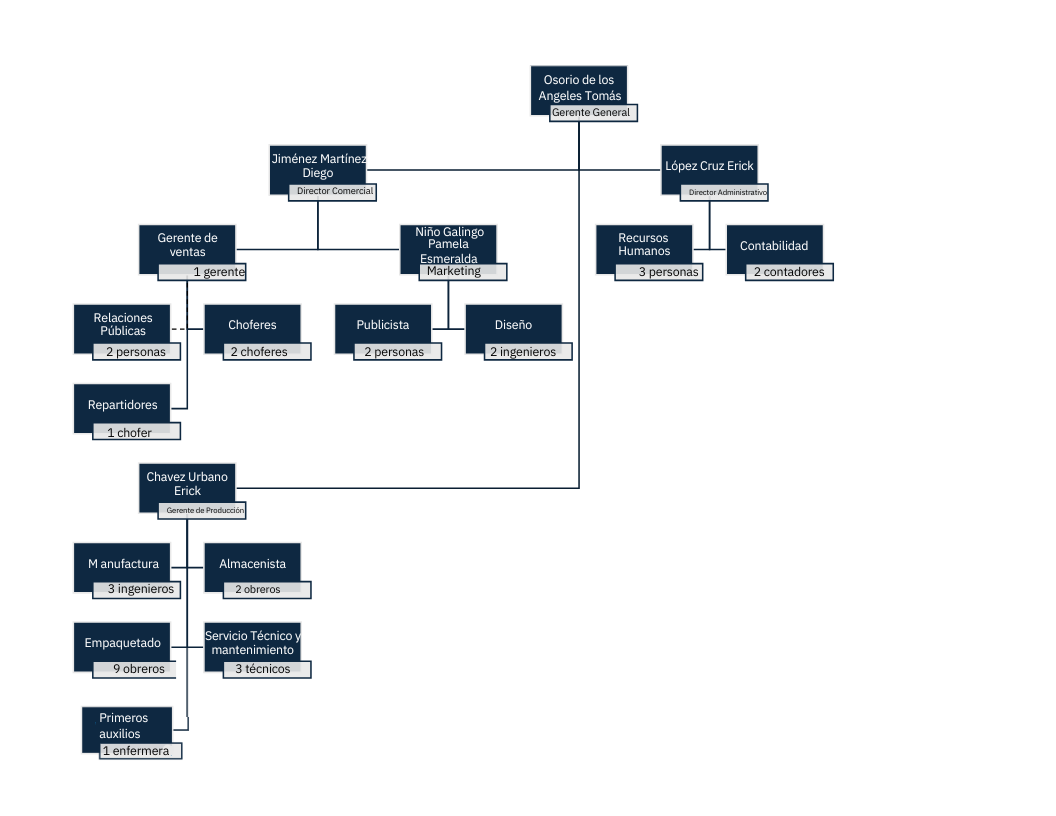
\includegraphics[width=1.3\textwidth]{img/Empresa/ORGANIGRAMA.png} 
    \caption{Se propone contratar menos ingenieros y más obreros o técnicos.}
\label{fig:macrolocalizacion}
\end{figure}

Además, se añadió un empleado destinado para primeros auxilios en el área de producción.
\newpage

\subsection{Descripción de funciones por área de operación}
\textbf{Personal administrativo}

\begin{longtable}[p]{ |p{2cm}||p{2cm}|p{4.5cm}|p{4.5cm}| }

 \hline
 Nombre del puesto & Jefe inmediato & Escolaridad & Descripción de funciones\\
 \hline
 \endfirsthead

 \hline
 Nombre del puesto & Jefe inmediato & Escolaridad & Descripción de funciones\\
 \hline
 \endhead
 
 \hline
 Director Comercial & Gerente General & Lic. en Adminstración de Empresas o área relacionada \newline Mtro. en Administrador de negocios (Deseable) &  Desarrollar y ejecutar estrategias comerciales para alcanzar los objetivos de ventas y crecimiento de la empresa.\\
 \hline
 Gerente de Ventas & Gerente General  & Lic. en Adminstración de Empresas o área relacionada &  Supervisar y capacitar al equipo de ventas, estableciendo
metas y evaluando el desempeño\newline Identificar oportunidades de crecimiento en
el mercado y desarrollar relaciones con clientes clave.\\
 \hline
 Gerente de Marketing & Gerente General & Lic. en Marketing, Comunicación, Administración de Empresas o carrera afín & Coordinar campañas
publicitarias, eventos promocionales y actividades de relaciones públicas.\\
 \hline
 Gerente de Recursos Humanos & Gerente General & Lic. en Administración de Empresas, Psicología Organizacional, Recursos Humanos o carrera afín & Gestionar el clima laboral y las relaciones
laborales, promoviendo un ambiente de trabajo positivo y colaborativo.\\
 \hline
 Gerente de Producción & Gerente General & Ing. Industrial, Mecatrónica o carrera afín & Desarrollar e implementar estrategias de mejora continua para incrementar la eficiencia operativa y la rentabilidad\\
 \hline
 
 \end{longtable}
 \newpage

\textbf{Personal de producción}

\begin{longtable}[p]{ |p{2cm}||p{2cm}|p{4.5cm}|p{4.5cm}| }

 \hline
 Nombre del puesto & Jefe inmediato & Escolaridad & Descripción de funciones\\
 \hline
 \endfirsthead

 \hline
 Nombre del puesto & Jefe inmediato & Escolaridad & Descripción de funciones\\
 \hline
 \endhead
 
 \hline
Obrero de producción\newline Técnico de producción & Gerente de Producción & Educación bachiller completa\newline Certificados de formación en áreas específicas de producción (deseable) & Operar maquinaria y equipos según los procedimientos establecidos\newline Realizar tareas manuales, como ensamblaje, empaque o carga y descarga de materiales\\
 \hline
 Repartidor\newline Chofer & Gerente de Producción &  Licencia de conducir vigente y categoría adecuada para vehículos de 2 toneladas & Conducir vehículos de reparto o transporte según las rutas establecidas y los horarios asignados\newline Cargar y descargar mercancías de manera segura y
 eficiente\newline Mantener el vehículo limpio y en buen estado de funcionamiento\\
 \hline
 Primeros Auxilios & Gerente de Producción &  Certificación en primeros auxilios\newline Lic. en Enfermería (Deseable) & Estar atento al estado de salud de los trabajadores en el área de producción\newline Proporcionar asistencia inmediata para lesiones menores, como cortes, raspaduras o quemaduras leves\newline Asegurarse de que el botiquín esté bien abastecido y en un lugar accesible\\
 \hline
\end{longtable}
\newpage

\textbf{Personal de mercadotecnia y ventas}

\begin{longtable}[p]{ |p{2cm}||p{2cm}|p{4.5cm}|p{4.5cm}| }

 \hline
 Nombre del puesto & Jefe inmediato & Escolaridad & Descripción de funciones\\
 \hline
 \endfirsthead

 \hline
 Nombre del puesto & Jefe inmediato & Escolaridad & Descripción de funciones\\
 \hline
 \endhead
 
 \hline

 Contador & Director Administrativo &  Lic. en Contaduría Pública, Administración de Empresas o carrera afín & Registrar y verificar en el sistema los movimientos y transacciones contables realizadas en la empresa\newline Revisar y señalar las variaciones encontradas con respecto a períodos anteriores\newline Registrar y balancear las entradas contables y las transacciones de intercambio semanal de pago a los bancos, relacionadas al Departamento de Servicios Internacionales\\
 \hline

\end{longtable}
\newpage

\subsection{Administración de personal}

\textbf{Planeación}

Para proyectar el crecimiento del personal, utilizamos el mismo porcentaje de crecimiento obtenido en la sección \textbf{Proyección de la Demanda}. en nuestro caso, utilizamos la fórmula aplicada a los valores existentes y obtenemos \[ Empleados = 33 + 2.7489x\]

\begin{tabular}{ |p{1cm}|p{2cm}|p{3cm}|p{3cm}|p{3cm}|  }
 \hline
 \multicolumn{5}{|c|}{PERSONAL\newline (Número de empleados)} \\
 \hline
 Año & Producción & Administración & Mercadotecnia y Ventas & Total de empleados\\
 \hline
 1 & 18 & 5 & 10 & 33\\
 \hline
 2 & 20 & 5 & 11 & 36\\
 \hline
 3 & 22 & 6 & 12 & 40\\
 \hline
 4 & 24 & 6 & 13 & 43\\
 \hline
 5 & 26 & 7 & 14 & 47\\
 \hline
 6 & 28 & 7 & 15 & 50\\
 \hline
\end{tabular}

\textbf{Reclutamiento}

El reclutamiento se hará de conocimiento a la población por medio de radio difusión, anuncios en puntos clave de la ciudad al igual que pancartas.

Como documentación general se solicitarán los siguientes documentos.

\begin{enumerate}
    \item Acta de Nacimiento
    \item CURP
    \item Número de Seguridad Social (NSS)
    \item Comprobante de Domicilio
    \item CV
    \item Certificados y Diplomas
    \item Cartas de Recomendación
\end{enumerate}

\textbf{Selección}

El personal de Recursos Humanos serán los encargados de realizar el proceso de selección en todo momento. A los aspirantes a puestos administrativos se le deberá realizar un examen de habilidades acorde a su área y estando relacionadas con las futuras actividades a realizar.

\begin{itemize}
    \item ¿Qué aspectos crees que te diferencian como ingeniero?
    \item ¿Cómo manejas situaciones de presión o crisis en un proyecto?
    \item ¿Qué producto crees que se comercializa mal?
    \item ¿Cuál es la última campaña de marketing que te llamó la atención?
    \item ¿Cuántos años de experiencia tienes como contador?
    \item ¿En qué áreas de la contabilidad te especializas?
    \item ¿Qué software contable has utilizado en tus trabajos anteriores?
\end{itemize}

\textbf{Contratación}

Primero se ofrecerá un contrato por un mes, dependiendo del desempeño se ofrecería posteriormente uno de 3 meses y finalmente un contrato indefinido. El puesto del empleado dependerá de su desempeño.

\textbf{Inducción}

Para el curso de inducción se ocupará medio día laboral completo, donde se le mostrará a los nuevos empleados las instalaciones de trabajo, medidas y procesos de seguridad, una breve introducción a su trabajo para finalmente asignarle el nuevo trabajador al encargado del área.

\textbf{Capacitación}

Al momento del arranque de operaciones, el personal administrativo será el primero en recibir la capacitación necesaria para procesos de manufactura, posteriormente se le impartirán estos cursos al personal restante dependiendo del cambio de empleados.

%%%%%%%%%%%%%%%%%%%%%%%%%%%%%%%%%%%%%%%
\section{Conclusiones del estudio administrativo}

La empresa tiene una misión y visión claramente definidas, enfocadas en la innovación, sostenibilidad y calidad. Sus valores fundamentales, como la innovación, calidad, sostenibilidad y colaboración, orientan todas sus actividades y decisiones estratégicas. Esta alineación entre misión, visión y valores asegura que la empresa mantenga un enfoque coherente en su desarrollo y crecimiento.

La estructura organizacional está bien definida, con roles y responsabilidades claramente asignados. Esto contribuye a una gestión financiera eficiente y a la minimización de riesgos. La propuesta de reducir el número de ingenieros y aumentar la mano de obra puede ser una estrategia eficaz para optimizar costos y mejorar la eficiencia operativa.

Las descripciones detalladas de los puestos aseguran que cada empleado conozca sus responsabilidades y objetivos. Esto es vital para el buen funcionamiento de la empresa y para mantener un ambiente laboral positivo y productivo. La planificación del crecimiento del personal, basada en la proyección de la demanda, muestra una estrategia proactiva para manejar el aumento de la carga de trabajo a medida que la empresa crece.

El estudio muestra que nuestra   empresa está bien posicionada para alcanzar sus objetivos de liderazgo en el mercado de cabinas para el cuidado de plantas. La clara definición de su filosofía, una estructura organizacional robusta y una planificación cuidadosa del personal son elementos clave para su éxito. Es fundamental que la empresa continúe monitoreando y ajustando sus estrategias según las dinámicas del mercado y las necesidades internas para mantener su competitividad y sostenibilidad a largo plazo.


\section{Marco jurídico para la puesta en marcha}


\subsection{Figura jurídica de la empresa}
La figura jurídica elegida para nuestra empresa, que se dedicará a la fabricación de cabinas climáticas para plantas, es la Sociedad de Responsabilidad Limitada (S. de R.L.). Esta decisión se basó en las ventajas que ofrece este tipo de sociedad, tales como la limitación de la responsabilidad de los socios al monto de sus aportaciones, la flexibilidad en la gestión y el capital inicial accesible.
\subsection{Requisitos para la constitución de la empresa}
Para constituir una Sociedad de Responsabilidad Limitada en México, se deben seguir los siguientes pasos:
\textbf{Autorización del nombre comercial:}
Obtener la autorización de la Secretaría de Economía para el uso del nombre comercial de la empresa, asegurando que no exista otra empresa con el mismo nombre. Este trámite se puede realizar en línea utilizando la e.firma.

\textbf{Elaboración del acta constitutiva:}
Con la asistencia de un notario, se debe elaborar el acta constitutiva de la empresa. Este documento establece los aspectos legales generales y particulares de la empresa, incluyendo el objeto social, capital social y normas de funcionamiento. Todos los socios deben firmar el acta.

\textbf{Aviso de uso de denominación:}
El funcionario que llevó a cabo la constitución de la sociedad debe informar a la Secretaría de Economía sobre las personas que se han asociado para crear la nueva empresa y el nombre que usarán, para evitar su uso por otras personas ajenas a la sociedad.

\textbf{Registro público de comercio:}
Inscribir la empresa en el Registro Público de Comercio, entidad que supervisa y protege a las empresas. Este trámite requiere el pago de derechos de inscripción, cuyo costo varía según el estado y el cual se especificará mas adelante \ref{sec:permisos}.

\textbf{Registro Federal de Contribuyentes (RFC):}
Realizar el trámite ante el Servicio de Administración Tributaria (SAT) para identificar la empresa como persona moral.

\textbf{Registro ante el IMSS:}
Registrarse en el Instituto Mexicano del Seguro Social (IMSS), incluso si los únicos trabajadores iniciales son los socios fundadores. No cumplir con este requisito puede resultar en multas.

\textbf{Inscripción en organismos adicionales:}
Inscribirse en otras instituciones según el tipo de actividad de la empresa, el municipio y el estado en el que se ubique. Esto puede incluir la Secretaría de Ecología y Medio Ambiente o el Instituto Mexicano de la Propiedad Intelectual, entre otros.

%Trámites de Licencia Municipal:
%a) Obtener la licencia municipal para la construcción de obra civil.
%b) Obtener la licencia municipal para el funcionamiento de la empresa, conforme a los reglamentos vigentes del municipio donde se establecerá la empresa.

\subsection{Elementos de un acta constitutiva}
El acta constitutiva es el documento obligatorio que da constancia y legalidad a la constitución de una sociedad al momento de crear una empresa. Este documento debe incluir los siguientes elementos:

\textbf{Datos de los constituyentes:}
Nombres, nacionalidad y domicilio de las personas físicas o morales que constituyen la sociedad.

\begin{itemize}
    \item Erick Chávez Urbano, Mexicana, Union y Progreso \#10 Cuilapam de Guerrero Oaxaca.
    \item Diego Jiménez Martínez, Mexicana, Privada de independencia \#26 Magdalena Etla.
    \item Pamela Esmeralda Galindo Niño, Mexicana, Privada de independencia \#40 Etla.
    \item Tomás Osorio de los Ángeles, Mexicana, Benito Juárez \#30, Acatlima Huajuapan.
    \item Erick López Cruz, Mexicana, Av. Modesto Seara Vásquez \#19
\end{itemize}

\textbf{Objeto social}
Descripción del objeto de la sociedad.

La sociedad tiene por objeto la realización de las siguientes actividades:
\begin{itemize}
    \item \textbf{Diseño, fabricación y comercialización de cabinas climáticas:} Diseñar, desarrollar, fabricar y comercializar cabinas climáticas para plantas, adecuadas para su uso en oficinas, hogares y cualquier otro espacio cerrado.
    \item \textbf{Instalación y mantenimiento de equipos:} Proveer servicios de instalación, mantenimiento preventivo y correctivo, así como la reparación de cabinas climáticas y otros sistemas relacionados con el control ambiental para plantas.
    \item \textbf{Investigación y desarrollo:} Realizar investigaciones y desarrollar nuevas tecnologías y métodos relacionados con el control climático, automatización y optimización del crecimiento de plantas en ambientes controlados.
    \item \textbf{Venta de accesorios y componentes:} Comercializar accesorios, componentes y repuestos necesarios para el funcionamiento y mantenimiento de las cabinas climáticas.
    \item \textbf{Capacitación y asesoría:} Ofrecer servicios de capacitación, asesoría técnica y consultoría a empresas, instituciones y particulares en relación con el uso, instalación y mantenimiento de las cabinas climáticas y otros sistemas de control ambiental.
    \item \textbf{Desarrollo de software y soluciones tecnológicas:} Desarrollar y comercializar software y soluciones tecnológicas que mejoren la eficiencia y funcionalidad de las cabinas climáticas, incluyendo sistemas de monitoreo y control remoto.
    \item \textbf{Importación y exportación:} Importar y exportar productos, materiales, equipos y tecnologías relacionados con las cabinas climáticas y el control ambiental para plantas.
    \item \textbf{Participación en proyectos y licitaciones:} Participar en proyectos, concursos, licitaciones y cualquier tipo de contratación pública o privada relacionada con la fabricación, instalación y mantenimiento de cabinas climáticas y sistemas de control ambiental.
\end{itemize}

\textbf{Razón social o denominación:}
El nombre bajo el cual operará la sociedad.
Nombre de la empresa: TerraGreen.

\textbf{Duración:}
Indefinido.

\textbf{Capital social:}
El importe del capital social, incluyendo las aportaciones de cada socio, ya sea en dinero o en otros bienes, y el criterio seguido para su valorización. Si el capital es variable, se debe indicar el mínimo establecido.

\begin{itemize}
    \item Erick Ch. -> \$ 5000
    \item Diego -> \$ 5000
    \item Esmeralda G. -> \$ 5000
    \item Tomás O. -> \$ 5000
    \item Erick Lo. -> \$ 5000
\end{itemize}

\textbf{Domicilio:}
El domicilio de la sociedad.

Colonia el Tepeyac, Juan Diego \#19, esquina con Díaz Ordaz, Huajuapan de león, Oaxaca, México.

\textbf{Administración:}
La manera en que se administrará la sociedad y las facultades de los administradores.

\textbf{Nombramiento de administradores:}
La designación de los administradores y los responsables de llevar la firma social.

\textbf{Distribución de utilidades y pérdidas:}
La manera de distribuir las utilidades y pérdidas entre los socios.

\textbf{Fondo de reserva:}
El importe del fondo de reserva es del 15\% de las ganancias anuales.

\textbf{Disolución anticipada:}
Los casos en que la sociedad puede disolverse anticipadamente.

\textbf{Liquidación:}
Las bases para la liquidación de la sociedad y el procedimiento para elegir a los liquidadores, si no fueron designados anticipadamente.

\subsection{Permisos municipales}
\label{sec:permisos}
\textbf{Licencia para construcción de una obra}
Los requisitos del municipio de Huajuapan de león pueden verse en el siguiente anexo \ref{sec:requisitosMunicipales}

El costo por permisos de construcción dependerán del tamaño de la obra y del municipio, varía entre un mínimo de \$471 y un máximo de \$7426 MXN. \cite{permisos2024Mexico}

\textbf{Licencia para el funcionamiento de la empresa}
A continuación se listan los documentos necesarios:
\begin{itemize}
    \item Acta constitutiva, original y 2 copias.
    \item Identificación oficial, original y 2 copias.
    \item RFC, original y 2 copias.
    \item Comprobante de domicilio, original y 2 copias.
    \item Croquis de ubicación, original y 2 copias.
    \item Comprobante de pago, original y 2 copias.
\end{itemize}

El pago correspondiente para este tipo de licencias varía según el municipio pero según el gobierno de méxico este monto corresponde a una cantidad de: \$ 3,211.00 MXN \cite{Licencia2024Mexico}


%\subsubsection{Licencia para la construcción de una obra civil}
%\subsubsection{Licencia para el funcionamiento de la empresa}

\section{Marco jurídico bajo el cual se regirán las operaciones de la empresa}

\subsection{ Normas Oficiales Mexicanas (NOMs)}

\textbf{Normas de Seguridad y Salud en el Trabajo}

NOM-001-STPS-2008: Edificios, locales, instalaciones y áreas en los centros de trabajo - Condiciones de seguridad.
Establece las condiciones de seguridad en las instalaciones laborales, que incluyen la infraestructura donde se encuentran las cámaras climáticas.

NOM-002-STPS-2010: Condiciones de seguridad - Prevención y protección contra incendios en los centros de trabajo.
Especifica las medidas para la prevención y protección contra incendios, relevante para la seguridad de las instalaciones.

NOM-022-STPS-2015: Electricidad estática en los centros de trabajo - Condiciones de seguridad.

\textbf{Normas Ambientales}

NOM-081-SEMARNAT-1994: Establece los límites máximos permisibles de emisión de ruido de las fuentes fijas y su método de medición.

Aplica si las cámaras climáticas generan ruido, asegurando que no excedan los límites permitidos.
NOM-085-SEMARNAT-2011: Contaminación atmosférica - Control de emisiones de fuentes fijas.

Regula las emisiones atmosféricas de fuentes fijas, pertinente si las cámaras climáticas utilizan sistemas que emiten contaminantes.

\textbf{Seguridad relacionadas con la electricidad estática}

Para cámaras climáticas, es posible que deban cumplirse varias NOMs dependiendo de sus características específicas, como:

NOM-024-SCFI-2013: Información comercial para empaques, instructivos y garantías de los productos electrónicos, eléctricos y electrodomésticos.

NOM-003-SCFI-2014: Productos eléctricos - Especificaciones de seguridad.

Recomendaciones
Revisión de Etiquetado y Publicidad: Asegurarse de que toda la información proporcionada sobre las cámaras climáticas sea veraz y suficiente.
Implementación de Garantías: Ofrecer garantías claras y cumplir con ellas de manera efectiva.
Atención al Cliente: Establecer un sistema eficiente para manejar quejas y reclamaciones.
Cumplimiento de NOMs: Identificar y cumplir con todas las NOMs aplicables a los productos.
Cumplir con la LFPC y las NOMs no solo es una obligación legal, sino que también contribuye a la confianza y satisfacción del consumidor, lo cual es vital para el éxito comercial de la empresa.

\textbf{Normas de Equipos y Productos}

NOM-003-SCFI-2014: Productos eléctricos - Especificaciones de seguridad.

Establece las especificaciones de seguridad para productos eléctricos, aplicable a los componentes eléctricos de las cámaras climáticas.

NOM-016-ENER-2016: Eficiencia energética de equipos y aparatos eléctricos - Límites, métodos de prueba y etiquetado.

Define los requisitos de eficiencia energética para equipos eléctricos, relevante para las cámaras climáticas que operan continuamente.



\subsection{Código de Comercio}

El contrato está regulado en los artículos 371 al 382 del Código de Comercio.

Definición y Alcance: El Código de Comercio regula los actos de comercio, las obligaciones de los comerciantes y las relaciones contractuales derivadas de estos actos. En este contexto, la fabricación y venta de cámaras climáticas se consideran actos de comercio.

Contratos Comerciales:

Compraventa Mercantil: El contrato de compraventa es uno de los más relevantes para la empresa fabricante de cámaras climáticas.  Define los derechos y obligaciones de las partes en una transacción comercial.

Contratos de Distribución y Agencia: También pueden ser relevantes para la comercialización de las cámaras climáticas. Aunque estos contratos no están específicamente definidos en el Código de Comercio, se regulan bajo las disposiciones generales de los contratos mercantiles.




 \subsection{Ley Federal de Protección al Consumidor (LFPC)}

La LFPC establece derechos y obligaciones tanto para los consumidores como para los proveedores de bienes y servicios, garantizando que los consumidores reciban productos y servicios de calidad, con información clara y veraz, y con la posibilidad de hacer valer sus derechos en caso de incumplimientos o abusos por parte de los proveedores.

Algunos puntos clave de la LFPC que pueden ser relevantes para la fabricación y comercialización de cámaras climáticas para flores incluyen:

Información y Publicidad: La ley exige que toda la información proporcionada sobre el producto sea clara, veraz y suficiente, evitando cualquier tipo de publicidad engañosa.

Garantías: Debes ofrecer garantías mínimas sobre la calidad y funcionalidad del producto.

Seguridad: Asegurar que los productos no representen un riesgo para la salud o seguridad de los consumidores.

Reclamaciones y Devoluciones: Establece procedimientos para que los consumidores puedan presentar quejas o reclamaciones y obtener compensaciones o devoluciones en caso de productos defectuosos o incumplimientos en las condiciones ofrecidas.

\section{Conclusiones del marco jurídico}

El marco jurídico establecido para la puesta en marcha de la empresa es sólido y bien fundamentado, asegurando que todas las bases legales necesarias estén cubiertas para iniciar operaciones con éxito.

La elección de la figura jurídica de Sociedad de Responsabilidad Limitada (S. de R.L.) es acertada, ya que ofrece ventajas significativas como la limitación de la responsabilidad de los socios al monto de sus aportaciones, flexibilidad en la gestión y un capital inicial accesible. Esto proporciona una estructura legal que protege a los socios y facilita la administración de la empresa.

El proceso detallado para la constitución de la empresa, que incluye desde la autorización del nombre comercial hasta la inscripción en el Registro Federal de Contribuyentes (RFC) y el Instituto Mexicano del Seguro Social (IMSS), asegura que la empresa cumpla con todos los requisitos legales y administrativos. Este enfoque meticuloso minimiza riesgos y garantiza el cumplimiento de las normativas vigentes.

El acta constitutiva, que incluye datos de los socios, el objeto social, la razón social, la duración de la sociedad, el capital social, el domicilio y la administración, establece una base legal clara y detallada para la operación de la empresa. La inclusión de todos estos elementos asegura que la empresa esté bien fundamentada y que los roles y responsabilidades de los socios y administradores estén claramente definidos. La obtención de permisos municipales necesarios para la construcción de una obra civil y el funcionamiento de la empresa demuestra un compromiso con el cumplimiento de las normativas locales, lo cual es crucial para la operación legal y ordenada de la empresa.

Finalmente, el marco jurídico bajo el cual se regirán las operaciones de la empresa, basado en el Código de Comercio, proporciona una estructura clara para la regulación de los actos de comercio, las obligaciones de los comerciantes y las relaciones contractuales. Los contratos comerciales específicos, como la compraventa mercantil y los contratos de distribución y agencia, están bien definidos, lo que facilita las transacciones comerciales y asegura que las relaciones con los clientes y distribuidores se manejen de manera legal y eficiente.
\chapter{Importancia del impacto ambiental}


El objetivo de la evaluación del impacto ambiental es la sustentabilidad, pero para que un proyecto sea sustentable debe considerar además de la factibilidad económica y el beneficio social, el aprovechamiento razonable de los recursos naturales (Ver Criterios de Sustentabilidad).

Procedimiento de Evaluación de Impacto Ambiental (PEIA).
La evaluación de un estudio de impacto ambiental lo realiza la autoridad mediante un procedimiento de tipo técnico administrativo,  hay tres opciones mediante las cuales puede presentarse dependiendo del control que se tenga sobre los impactos y la magnitud del área donde se pretende desarrollar un proyecto:  

 a).-	 Informe preventivo
 b).-	 Manifestación de impacto ambiental modalidad particular y,
 c).-	 Manifestación de impacto ambiental modalidad regional.
a).- Informe preventivo

Requieren de presentar un Informe Preventivo y no una Manifestación de Impacto Ambiental en los siguientes casos:  

I.- Existan normas oficiales mexicanas u otras disposiciones que regulen las emisiones, las descargas, el aprovechamiento de recursos naturales y, en general, todos los impactos ambientales relevantes que puedan producir las obras o actividades;

II.- Las obras o actividades de que se trate estén expresamente previstas por un plan parcial de desarrollo urbano o de ordenamiento ecológico que haya sido evaluado por la Secretaría en los términos del artículo siguiente, o 

III.- Se trate de instalaciones ubicadas en parques industriales autorizados en los términos de la presente sección.

En los casos anteriores, la Secretaría, una vez analizado el informe preventivo, determinará, en un plazo no mayor de veinte días, si se requiere la presentación de una manifestación de impacto ambiental en alguna de las modalidades o si se está en alguno de los supuestos señalados.

b y c ).- Manifestación de Impacto Ambiental (MIA)

Se trata de un documento con base en estudios técnicos con el que las personas (físicas o morales) que desean realizar alguna de las obras o actividades previstas en el artículo 28 de la  LGEEPA, analizan y describen las condiciones ambientales anteriores a la realización del proyecto con la finalidad de evaluar  los impactos potenciales que la construcción y operación de dichas obras o la realización de las actividades podría causar al ambiente  y definir y proponer las medidas necesarias para prevenir, mitigar o compensar esas alteraciones.

\section{Objetivos 2030 que contribuye la empresa}

ODS 2: Hambre Cero

Contribución: Las cámaras climáticas pueden ser utilizadas para optimizar el crecimiento de flores comestibles y otras plantas, ayudando a mejorar la seguridad alimentaria y la nutrición en ciertas regiones.


ODS 8: Trabajo Decente y Crecimiento Económico

Contribución: Al proporcionar tecnología avanzada para la conservación y el cultivo de flores, la empresa puede fomentar el crecimiento económico en el sector agrícola y floricultor, creando empleos y mejorando las condiciones laborales.


ODS 9: Industria, Innovación e Infraestructura

Contribución: La empresa puede impulsar la innovación en la industria floricultora al introducir cámaras climáticas avanzadas, promoviendo la investigación y el desarrollo en tecnología agrícola.


ODS 12: Producción y Consumo Responsables

Contribución: Las cámaras climáticas ayudan a reducir el desperdicio de flores al optimizar su conservación y transporte, promoviendo prácticas de producción y consumo más sostenibles.


ODS 13: Acción por el Clima

Contribución: Al proporcionar soluciones para el control climático, la empresa contribuye a la adaptación y mitigación del cambio climático, permitiendo a los productores de flores reducir su huella de carbono mediante el uso eficiente de recursos.


ODS 15: Vida de Ecosistemas Terrestres

Contribución: Las cámaras climáticas pueden ayudar a preservar especies de flores raras y en peligro de extinción, promoviendo la biodiversidad y la conservación de los ecosistemas terrestres.


ODS 17: Alianzas para Lograr los Objetivos


Contribución: La empresa puede formar alianzas con organizaciones no gubernamentales, instituciones de investigación y otras empresas para promover el desarrollo sostenible en la floricultura y compartir conocimientos y tecnología.

Estas contribuciones muestran cómo una empresa dedicada a la venta de cámaras climáticas para flores puede alinear sus operaciones y objetivos con los ODS, promoviendo prácticas sostenibles y responsables en su industria.

\section{Aplicación de las leyes nacionales}


Como empresa nos aseguramos de cumplir con todas las regulaciones ambientales aplicables a su operación, lo cual incluye la obtención de permisos, la realización de evaluaciones de impacto ambiental, el control de emisiones y la gestión adecuada de residuos, entre otros aspectos. Para un cumplimiento adecuado, es recomendable contar con asesoría legal y ambiental especializada.

\subsection{Ley General de Equilibrio Ecológico y la Protección al Ambiente}

La LGEEPA establece que cualquier proyecto que pueda causar desequilibrio ecológico significativo debe someterse a una Evaluación de Impacto Ambiental (EIA). Esto incluye la instalación y operación de cámaras climáticas, ya que pueden tener implicaciones sobre el uso de energía, generación de residuos y emisiones atmosféricas.

Emisiones Atmosféricas: La empresa debe cumplir con las normas oficiales mexicanas (NOM) que regulan las emisiones de contaminantes al aire. Es posible que las cámaras climáticas utilicen sistemas de refrigeración y climatización que generen emisiones.

Residuos: La generación y manejo de residuos peligrosos y no peligrosos están regulados por la LGEEPA y otras leyes como la Ley General para la Prevención y Gestión Integral de los Residuos (LGPGIR).

Eficiencia Energética: Las cámaras climáticas deben diseñarse y operarse de manera que optimicen el consumo de energía. La NOM-ENER y otras regulaciones energéticas pueden ser aplicables.

Consumo de Agua: Si las cámaras utilizan agua para la humidificación o refrigeración, deben implementarse prácticas para su uso eficiente y cumplir con las normativas de la Comisión Nacional del Agua (CONAGUA).

La empresa es responsable de cualquier daño ambiental que pueda causar y debe implementar medidas de mitigación, restauración y compensación según lo establecido por la LGEEPA.

\subsection{Ley Federal de Responsabilidad Ambiental}

La empresa debe realizar una evaluación de impacto ambiental (EIA) para identificar, prevenir y mitigar posibles impactos ambientales negativos derivados de sus actividades. Esto es especialmente relevante si la instalación de las cámaras climáticas implica la modificación de ecosistemas naturales o la emisión de contaminantes.

Debe implementar medidas para prevenir y controlar la contaminación del aire, agua y suelo. La LFRA obliga a las empresas a adoptar tecnologías limpias y prácticas sostenibles para minimizar su huella ambiental.

En caso de que se produzca un daño ambiental, la empresa está obligada a repararlo. La LFRA establece mecanismos para que las autoridades ambientales exijan la reparación del daño y, en su caso, impongan sanciones.

La aplicación de la LFRA y otras leyes ambientales es esencial para garantizar que las operaciones de la empresa no dañen el entorno y para evitar sanciones legales.

\subsection{Ley General para la Prevención y Gestión Integral de los Residuos}

Informes de Cumplimiento Ambiental: La empresa deberá presentar informes periódicos a la Secretaría de Medio Ambiente y Recursos Naturales (SEMARNAT) y a otras autoridades competentes sobre el cumplimiento de las normas y regulaciones ambientales.

NOM-052-SEMARNAT-2005: Identificación y listado de los residuos peligrosos.

NOM-059-SEMARNAT-2010: Protección ambiental-especies nativas de México de flora y fauna silvestres-categorías de riesgo y especificaciones para su inclusión, exclusión o cambio-lista de especies en riesgo.

NOM-138-SEMARNAT/SSA1-2012: Límites máximos permisibles de hidrocarburos en suelos y las especificaciones para su caracterización y remediación.

\chapter{Estudio económico y evaluación económica}

\section{Presupuesto de Costos de producción}

Para la producción durante cada año se incluyen  costos de materiales, mano de obra directa e indirecta, gastos generales de fabricación, entre otros.
Cada categoría de costos se desglosa para mostrar su contribución total al costo de producción por año.

\begin{figure}[H]
    \centering	
    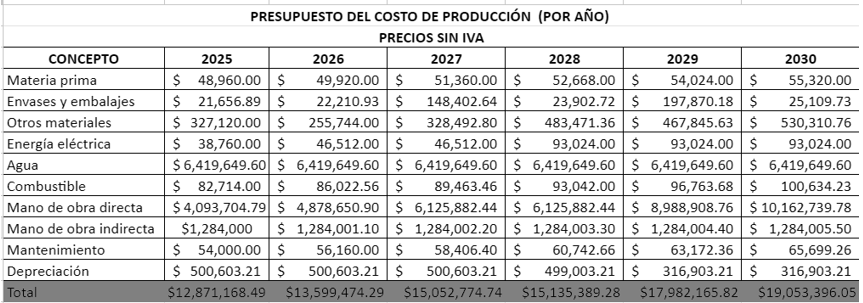
\includegraphics[width=.7\textwidth]{chapters/ELC_1.png} 
    \caption{Presupuesto de costo de producción}
\label{fig:macrolocalizacion}
\end{figure}


\begin{figure}[H]
    \centering	
    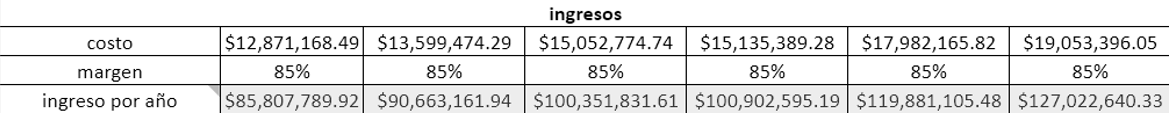
\includegraphics[width=.7\textwidth]{chapters/ELC_2.png} 
    \caption{Ingresos}
\label{fig:macrolocalizacion}
\end{figure}

Esta tabla indica la cantidad total de unidades producidas durante cada período de dos años. Es útil para entender la capacidad de producción utilizada y las fluctuaciones en la demanda a lo largo del tiempo.


\begin{figure}[H]
    \centering	
    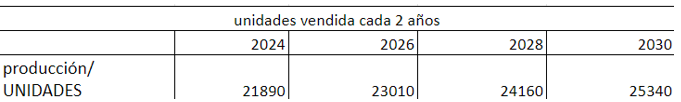
\includegraphics[width=.5\textwidth]{chapters/ELC_3.png} 
    \caption{Unidades de producción}
\label{fig:macrolocalizacion}
\end{figure}

Cada una de estas tablas proporciona información clave para evaluar el desempeño financiero y operativo de la empresa, ayudando a identificar tendencias, eficiencias y áreas de mejora en la gestión de costos, ingresos y producción.

\section{Presupuesto de gastos de administración}


Para realizar el presupuesto se consideraron :Salarios y Honorarios.

Personal Administrativo: Sueldos del personal administrativo responsable de la gestión del proyecto.

Consultores y Asesores: Honorarios para expertos que brinden asesoramiento específico sobre aspectos técnicos, financieros o legales del proyecto.

\begin{figure}[H]
    \centering	
    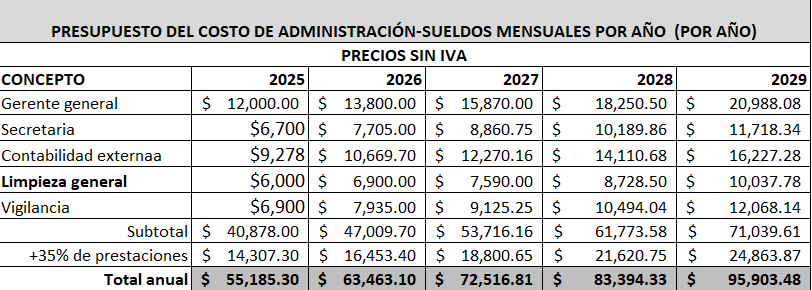
\includegraphics[width=.7\textwidth]{chapters/ELC_4.png} 
    \caption{Presupuestos de administración-sueldos}
\label{fig:macrolocalizacion}
\end{figure}

\begin{figure}[H]
    \centering	
    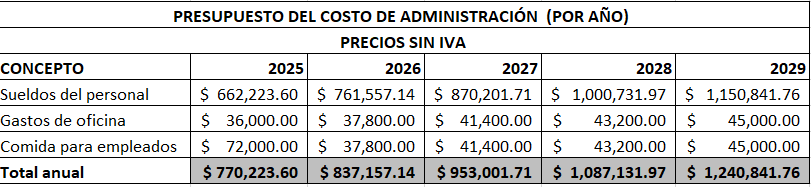
\includegraphics[width=.7\textwidth]{chapters/ELC_5.png} 
    \caption{Presupuestos de administración}
\label{fig:macrolocalizacion}
\end{figure}



\section{Presupuesto de gastos de venta}

Para el presupuesto de gastos para realizar la venta se consideró lo necesario para poder ofrecer el producto y este sea llevado con éxito al cliente, para ello se contempló el gerente de ventas, ingenieros, obreros, choferes, contadores y auxiliares.

\begin{figure}[H]
    \centering	
    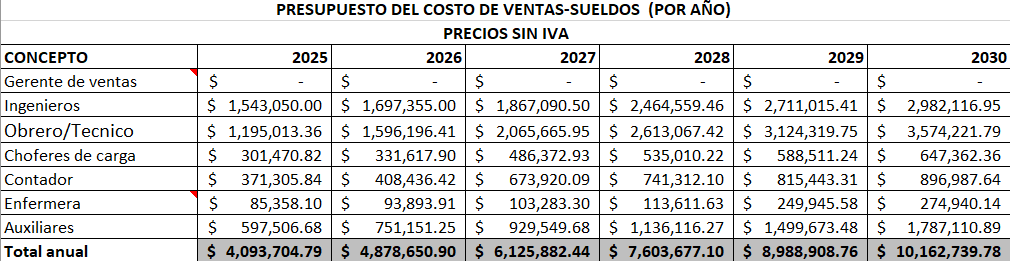
\includegraphics[width=.9\textwidth]{chapters/ELC_6.png} 
    \caption{Presupuestos de ventas-sueldos}
\label{fig:macrolocalizacion}
\end{figure}

\begin{figure}[H]
    \centering	
    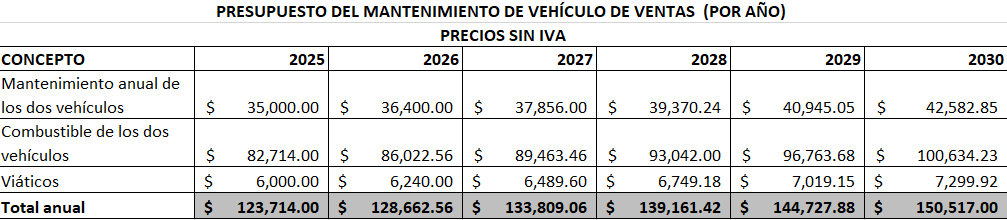
\includegraphics[width=.8\textwidth]{chapters/ELC_7.png} 
    \caption{resupuesto de mantenimiento de vehículo de ventas}
\label{fig:macrolocalizacion}
\end{figure}

\begin{figure}[H]
    \centering	
    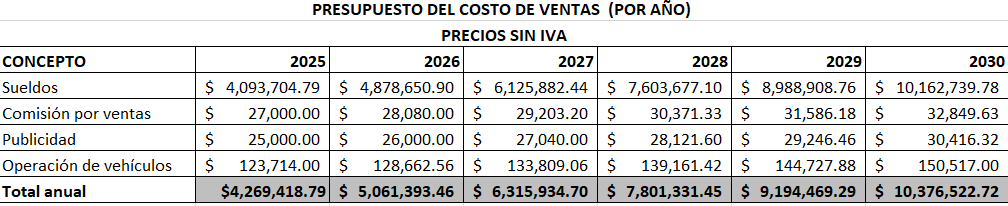
\includegraphics[width=.8\textwidth]{chapters/ELC_8.png} 
    \caption{Presupuestos de costo de ventas}
\label{fig:macrolocalizacion}
\end{figure}


\section{Costo total de operación de la empresa}

\begin{figure}[H]
    \centering	
    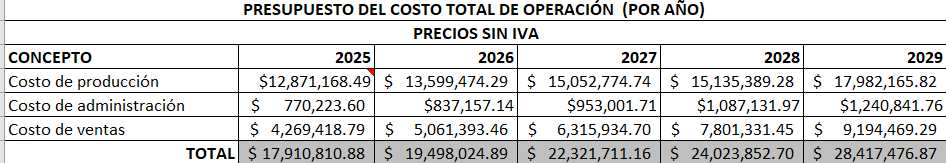
\includegraphics[width=.7\textwidth]{chapters/ELC_9.png} 
    \caption{Costo total de operación}
\label{fig:macrolocalizacion}
\end{figure}




\section{Inversión inicial en activo fijo y diferido}






\subsection{ Inversión fija}

A continuación, se presenta un análisis de inversión fija basándonos en
los documentos y con la investigación de los precios actuales según las
entidades correspondientes al concepto se realizaron los cálculos en los
apartados siguientes.

\subsubsection{Adquisición del terreno }


\hspace{1cm}

\begin{quote}


\textbf{Costo del terreno y gastos por adquisición}

El las siguientes tablas se presentas los debidos costos que se pagaran
para el tramite de la propiedad el cual se realizaran los tramites en
menos de un mes considerando que se tengan los papeles correspondientes
y no se presente algún inconveniente.
\hspace{1cm}


\end{quote}

\begin{longtable}[]{@{}
  >{\raggedright\arraybackslash}p{(\columnwidth - 8\tabcolsep) * \real{0.4331}}
  >{\raggedright\arraybackslash}p{(\columnwidth - 8\tabcolsep) * \real{0.1227}}
  >{\raggedright\arraybackslash}p{(\columnwidth - 8\tabcolsep) * \real{0.1562}}
  >{\raggedright\arraybackslash}p{(\columnwidth - 8\tabcolsep) * \real{0.1337}}
  >{\raggedright\arraybackslash}p{(\columnwidth - 8\tabcolsep) * \real{0.1543}}@{}}
\toprule()
\begin{minipage}[b]{\linewidth}\raggedright
\textbf{CONCEPTO}
\end{minipage} & \begin{minipage}[b]{\linewidth}\raggedright
\textbf{UNIDAD}
\end{minipage} & \begin{minipage}[b]{\linewidth}\raggedright
\textbf{CANTIDAD}
\end{minipage} & \begin{minipage}[b]{\linewidth}\raggedright
\textbf{P.U}
\end{minipage} & \begin{minipage}[b]{\linewidth}\raggedright
\textbf{TOTAL}
\end{minipage} \\
\midrule()
\endhead
Terreno & M2 & 560 & \$1600 & \$896 000 \\
& & & \textbf{Sub total} & \$896 000 \\
\textbf{Escrituración} & & & & \\
Avaluó de inmuebles & \% & 0.13 & \$896 000 & \$1164.8 \\
Adquisición de inmuebles ABI & \% & 2.0 & \$896 000 & \$17920 \\
Certificado de libertad de gravámenes & Tramite & 1.0 & \$100 & \$100 \\
Gastos de papeleo y copias en la notaria & Tramite & 1.0 & \$900 &
\$900 \\
Avisos preventivos y certificados & Tramite & 1.0 & \$500 & \$500 \\
Inscripción al registro publico de la propiedad & \% & 0.075 & \$896 000
& \$672 \\
Honorarios del notario & \% & 1.5 & \$450 000 & \$13440 \\
\multicolumn{3}{@{}>{\raggedright\arraybackslash}p{(\columnwidth - 8\tabcolsep) * \real{0.7120} + 4\tabcolsep}}{%
\multirow{2}{*}{}} & \textbf{Sub total} & \$34696.8 \\
& & & \textbf{TOTAL} & \$930 696.8 \\
\bottomrule()
\end{longtable}

\begin{quote}

Costos y gastos de adquisición

La tabla presentaba anteriormente cubre los costos para la escrituración
dando un total de \$930 696.8 esto es sin contemplar la urbanización,
promediando la realización de este en un mes.

Para el siguiente mes se realizará la urbanización entre los cuales se
incluirán necesariamente los siguientes conceptos.

\hspace{2cm}

\textbf{Costos por permisos y licencias}
\end{quote}

\begin{longtable}[]{@{}
  >{\raggedright\arraybackslash}p{(\columnwidth - 8\tabcolsep) * \real{0.4605}}
  >{\raggedright\arraybackslash}p{(\columnwidth - 8\tabcolsep) * \real{0.1240}}
  >{\raggedright\arraybackslash}p{(\columnwidth - 8\tabcolsep) * \real{0.1579}}
  >{\raggedright\arraybackslash}p{(\columnwidth - 8\tabcolsep) * \real{0.1227}}
  >{\raggedright\arraybackslash}p{(\columnwidth - 8\tabcolsep) * \real{0.1348}}@{}}
\toprule()
\begin{minipage}[b]{\linewidth}\raggedright
\textbf{CONCEPTO}
\end{minipage} & \begin{minipage}[b]{\linewidth}\raggedright
\textbf{UNIDAD}
\end{minipage} & \begin{minipage}[b]{\linewidth}\raggedright
\textbf{CANTIDAD}
\end{minipage} & \begin{minipage}[b]{\linewidth}\raggedright
\textbf{P.U}
\end{minipage} & \begin{minipage}[b]{\linewidth}\raggedright
\textbf{TOTAL}
\end{minipage} \\
\midrule()
\endhead
Lotificación & M2 & 7000 & 2 & \$14 000 \\
Costo por cada lote resultante (en este caso 2) & Lote & 2 & 500 & \$1
000 \\
Aprobación del proyecto & M2 & \$896 000 & 0.6 & \$5376 \\
Uso del suelo & M2 & \$896 000 & 1.6 & \$14336 \\
Licencia de construcción de la barda & M2 & \$896 000 & 7.5 & \$36000 \\
\multicolumn{4}{@{}>{\raggedright\arraybackslash}p{(\columnwidth - 8\tabcolsep) * \real{0.8652} + 6\tabcolsep}}{%
} & \$70712 \\
\bottomrule()
\end{longtable}

\hspace{1cm}


\begin{quote}
Costos por permisos y licencias

\textbf{Costos de urbanización por partida}
\end{quote}

\begin{longtable}[]{@{}
  >{\raggedright\arraybackslash}p{(\columnwidth - 4\tabcolsep) * \real{0.3375}}
  >{\raggedright\arraybackslash}p{(\columnwidth - 4\tabcolsep) * \real{0.3269}}
  >{\raggedright\arraybackslash}p{(\columnwidth - 4\tabcolsep) * \real{0.3356}}@{}}
\toprule()
\begin{minipage}[b]{\linewidth}\raggedright
Partida
\end{minipage} & \begin{minipage}[b]{\linewidth}\raggedright
\%
\end{minipage} & \begin{minipage}[b]{\linewidth}\raggedright
costo/M2
\end{minipage} \\
\midrule()
\endhead
Agua potable & 11.0\% & \$150 250 \\
Condiciones generales & 9.5\% & \$250 251 \\
Drenaje pluvial & 2.3\% & \$75 256 \\
Electrificado y alumbrado & 5.2\% & \$132 025 \\
Terracerías & 6.2\% & \$145 256 \\
Pavimentos y banquetas & 4.1\% & \$128 185 \\
Totales & & \$881 223 \\
\bottomrule()
\end{longtable}

\begin{quote}
Costos de urbanización por m2

Los apartados anteriores forman partes de la inversión para la
adquisición del terreno y puesta en marcha para el inicio de la
construcción de la planta a lo cual el costo total es englobado en la
siguiente tabla.

\hspace{1cm}

\newpage

\textbf{Costo total del terreno más adquisición}
\end{quote}

\begin{longtable}[]{@{}
  >{\raggedright\arraybackslash}p{(\columnwidth - 4\tabcolsep) * \real{0.3377}}
  >{\raggedright\arraybackslash}p{(\columnwidth - 4\tabcolsep) * \real{0.3305}}
  >{\raggedright\arraybackslash}p{(\columnwidth - 4\tabcolsep) * \real{0.3319}}@{}}
\toprule()
\begin{minipage}[b]{\linewidth}\raggedright
CONCEPTO
\end{minipage} & \begin{minipage}[b]{\linewidth}\raggedright
\%
\end{minipage} & \begin{minipage}[b]{\linewidth}\raggedright
TOTAL
\end{minipage} \\
\midrule()
\endhead
Adquisición del terreno & & \$896 000 \\
Escrituras y tramites & & \$34 696.8 \\
Urbanización y lotificación & & \$881 223 \\
Construcción de barda & & \$150 254 \\
Proyecto ejecutivo & & \$120 581 \\
Permisos y licencias & & \$72 252 \\
\textbf{Total} & \textbf{100\%} & \textbf{\$2 155 006.8} \\
\bottomrule()
\end{longtable}

\begin{quote}
Costos totales de adquisición del terreno

El costo total para iniciar con la construcción de la planta será de
\textbf{\$2 155 006.8} teniendo el capital para la inversión cubriendo
en su totalidad el pago sin requerir por esta vez la solicitud de un
préstamo bancario o externo, disminuyendo el precio para poder invertir
en los demás aspectos.

4.2. Obra civil.
\end{quote}

En este apartado se realizan los presupuestos poyados por la
documentación generado por arquitectos y constructores sobre el cual se
genera un documento con los requerimientos específicos, ¡normativas,
materiales, presupuestos usos del espacio y tecnología a utilizar.

\begin{longtable}[]{@{}
  >{\raggedright\arraybackslash}p{(\columnwidth - 4\tabcolsep) * \real{0.2311}}
  >{\raggedright\arraybackslash}p{(\columnwidth - 4\tabcolsep) * \real{0.1361}}
  >{\raggedright\arraybackslash}p{(\columnwidth - 4\tabcolsep) * \real{0.6327}}@{}}
\toprule()
\multicolumn{3}{@{}>{\raggedright\arraybackslash}p{(\columnwidth - 4\tabcolsep) * \real{1.0000} + 4\tabcolsep}@{}}{%
\begin{minipage}[b]{\linewidth}\raggedright
\textbf{Proyecto de construcción}
\end{minipage}} \\
\midrule()
\endhead
\multicolumn{3}{@{}>{\raggedright\arraybackslash}p{(\columnwidth - 4\tabcolsep) * \real{1.0000} + 4\tabcolsep}@{}}{%
\textbf{Proyecto de planta}} \\
\multicolumn{3}{@{}>{\raggedright\arraybackslash}p{(\columnwidth - 4\tabcolsep) * \real{1.0000} + 4\tabcolsep}@{}}{%
\textbf{Área total del lote} 560 m\textsuperscript{2} \textbf{Área de
planta baja} 250 m\textsuperscript{2}

\textbf{Área de construcción} 360 m\textsuperscript{2} \textbf{Áreas de
planta alta} 110 m\textsuperscript{2}} \\
\multicolumn{3}{@{}>{\raggedright\arraybackslash}p{(\columnwidth - 4\tabcolsep) * \real{1.0000} + 4\tabcolsep}@{}}{%
\textbf{Primer nivel-Distribución}} \\
Comedor & 18.6m\textsuperscript{2} &
\multirow{13}{*}{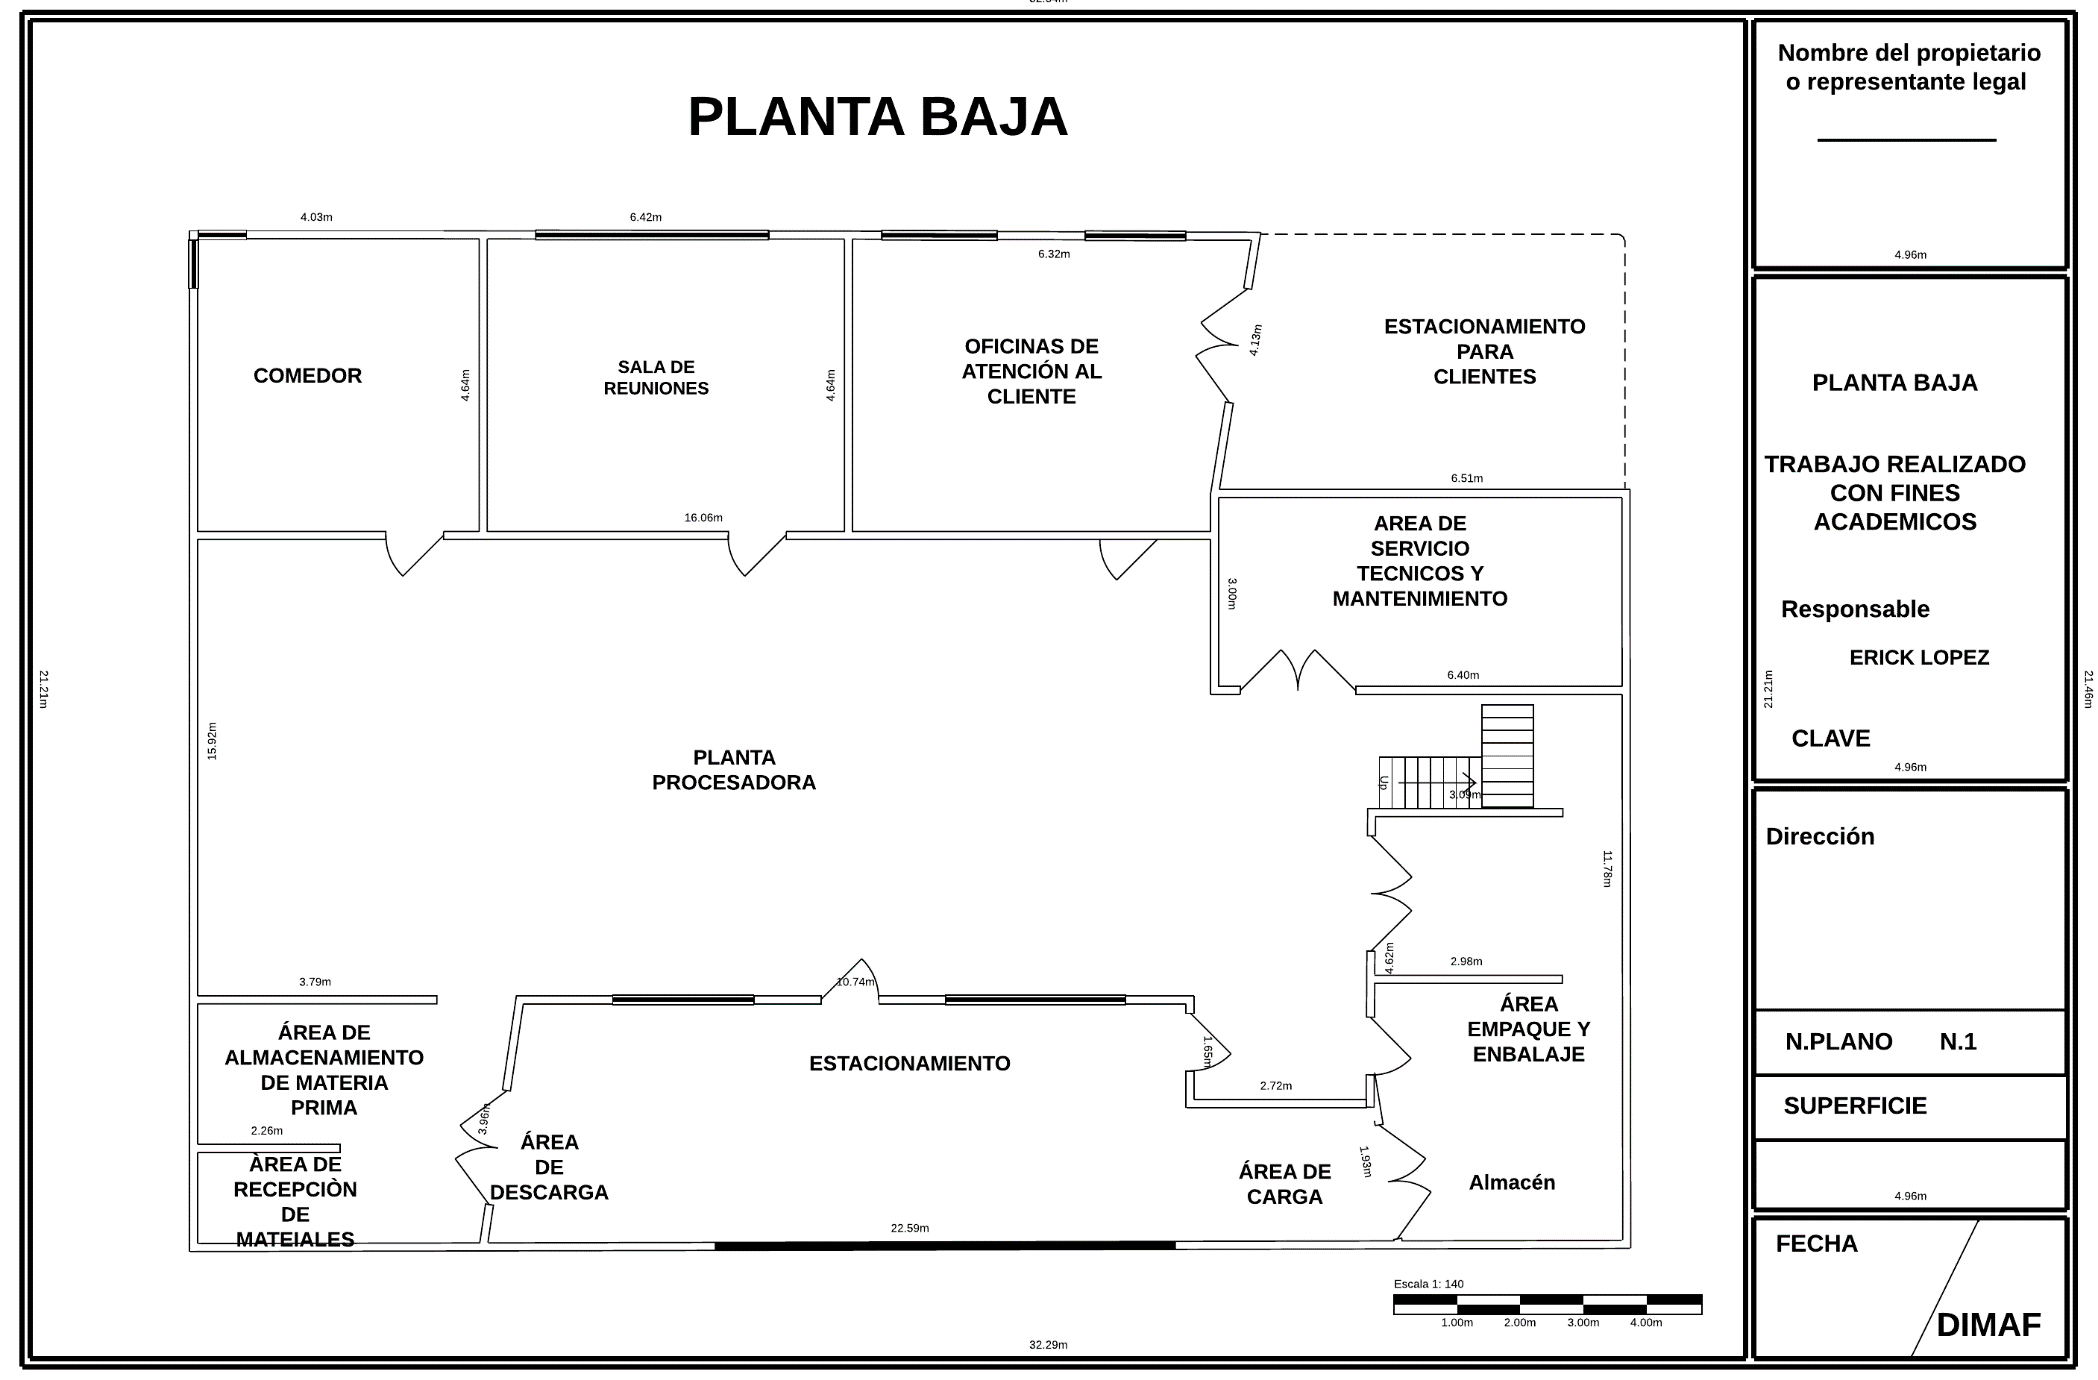
\includegraphics[width=4.22565in,height=3.04844in]{chapters/image1_.png}

} \\

Oficina de atención al cliente & 29.78m\textsuperscript{2} \\
Estacionamiento de clientes & 26.88m\textsuperscript{2} \\
Área de servicio técnico y mantenimiento & 19.2m\textsuperscript{2} \\
Área de empaque y embalaje & 6m\textsuperscript{2} \\
Almacén & 9m\textsuperscript{2} \\
Área de carga & 6m\textsuperscript{2} \\
Área de descarga & 10m\textsuperscript{2} \\
Estacionamiento para la empresa & 30m\textsuperscript{2} \\
Área de recepción de materiales & 6m\textsuperscript{2} \\
Área de almacenamiento de materias prima & 12m\textsuperscript{2} \\
Sala de reuniones & 28m\textsuperscript{2} \\
Planta procesadora & 370m\textsuperscript{2} \\
\multicolumn{3}{@{}>{\raggedright\arraybackslash}p{(\columnwidth - 4\tabcolsep) * \real{1.0000} + 4\tabcolsep}@{}}{%


\textbf{Segundo nivel-Distribución}} \\
Oficina 1 & 20m\textsuperscript{2} &
\multirow{4}{*}
{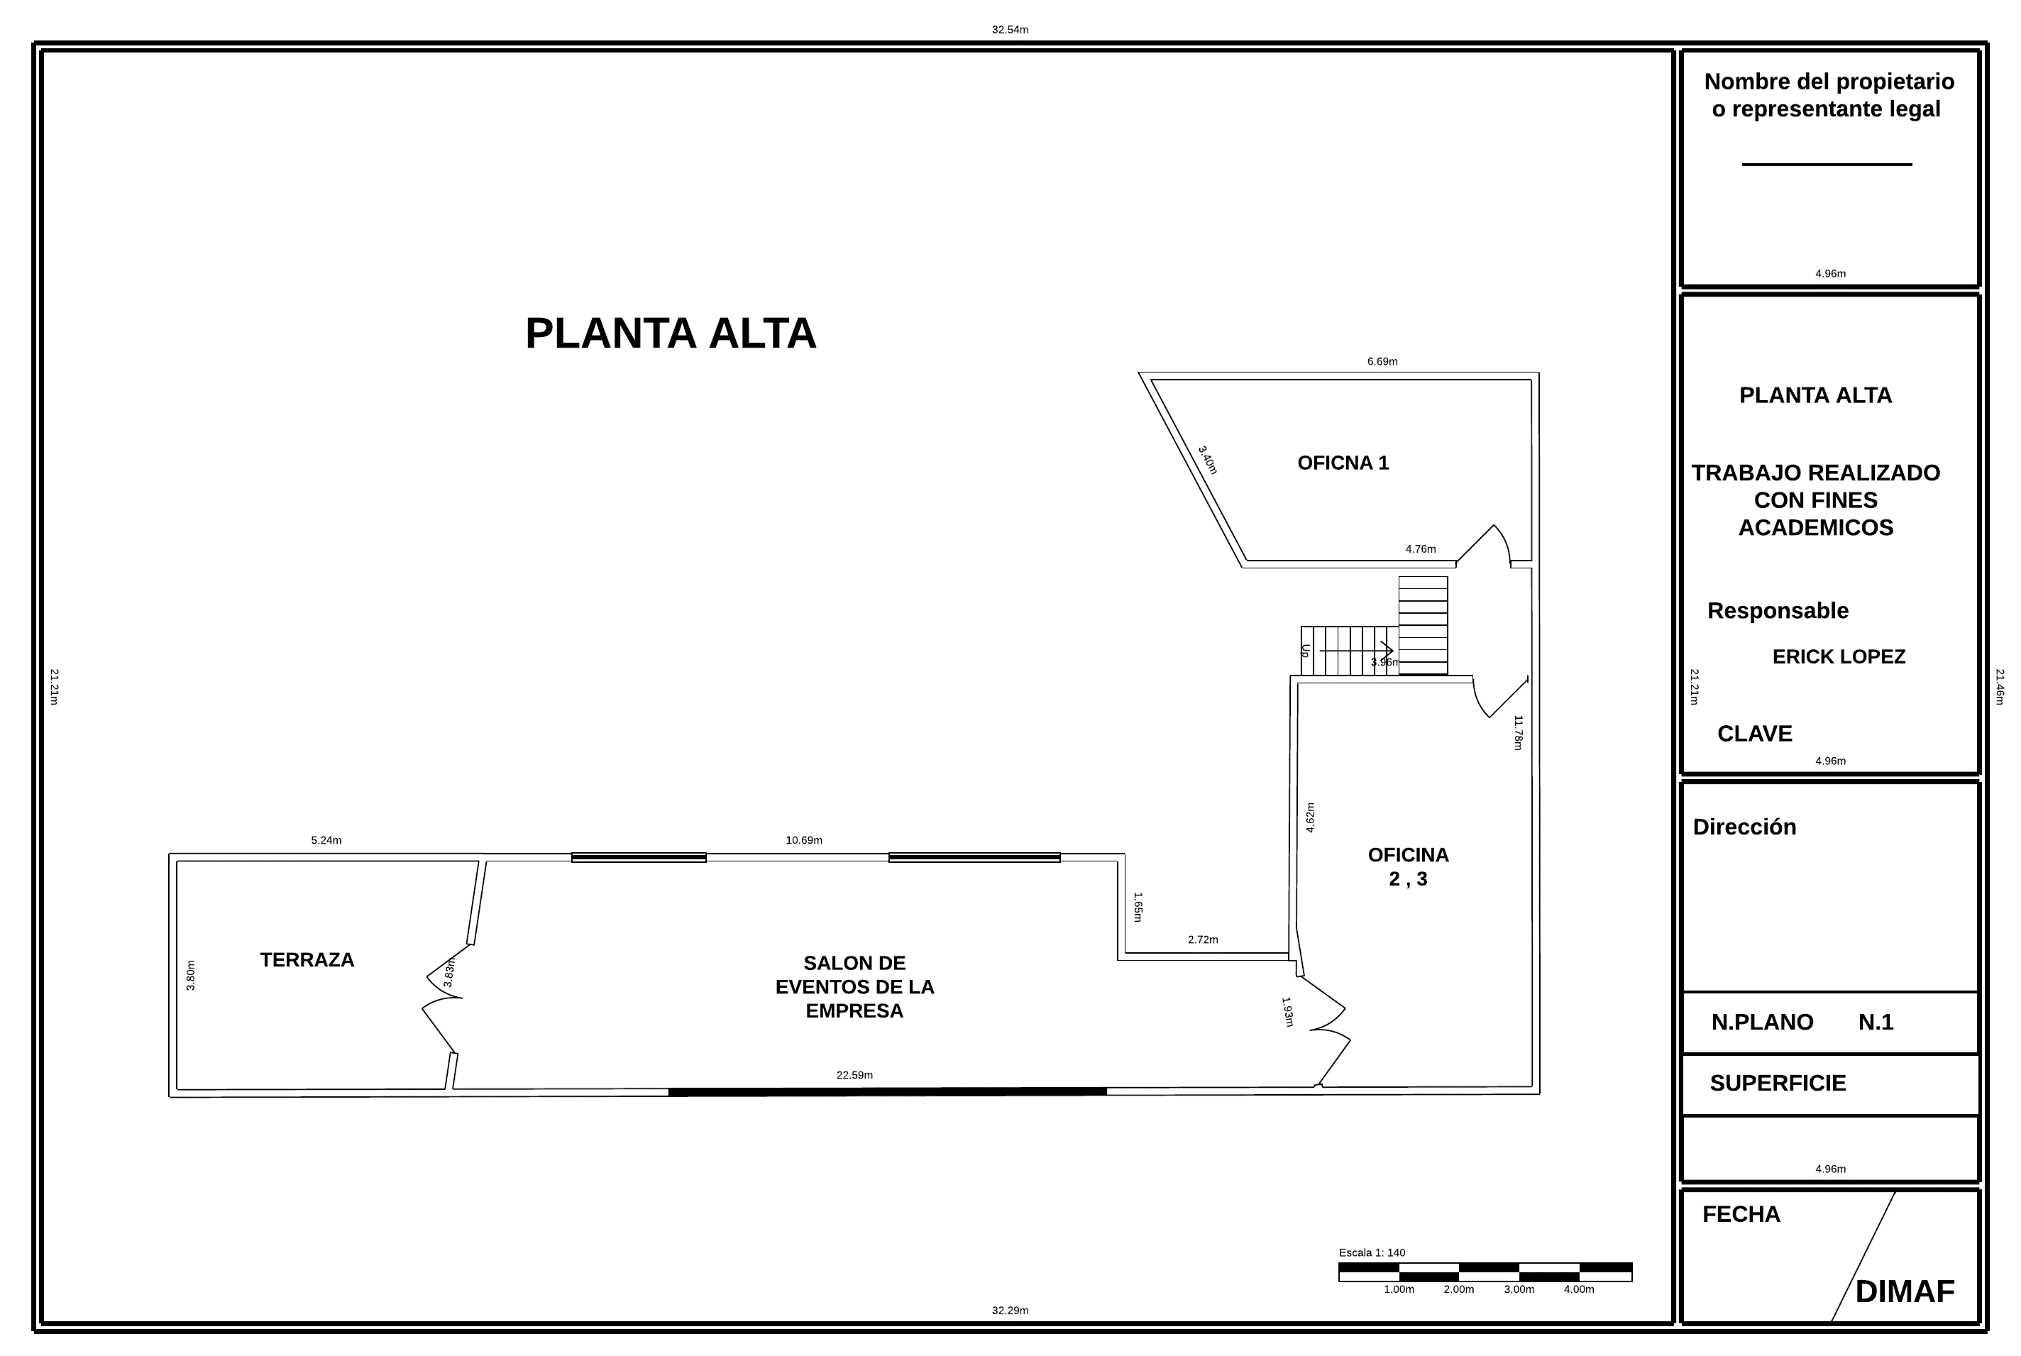
\includegraphics[width=3.95825in,height=2.13528in]{chapters/image2_.png}} \\
\hspace{2cm}
Oficina 2,3 & 39.2m\textsuperscript{2} \\
Salón de eventos & 42.2m\textsuperscript{2} \\
Terraza & 20.1m\textsuperscript{2} \\
\hspace{4cm}
\bottomrule()
\end{longtable}


\hspace{2cm}

Características geométricas de la distribución de los departamentos de
la empresa. Elaboración propia.







\subsubsection{Obra civil}




\subsection{Obra civil}

\begin{figure}[H]
    \centering	
    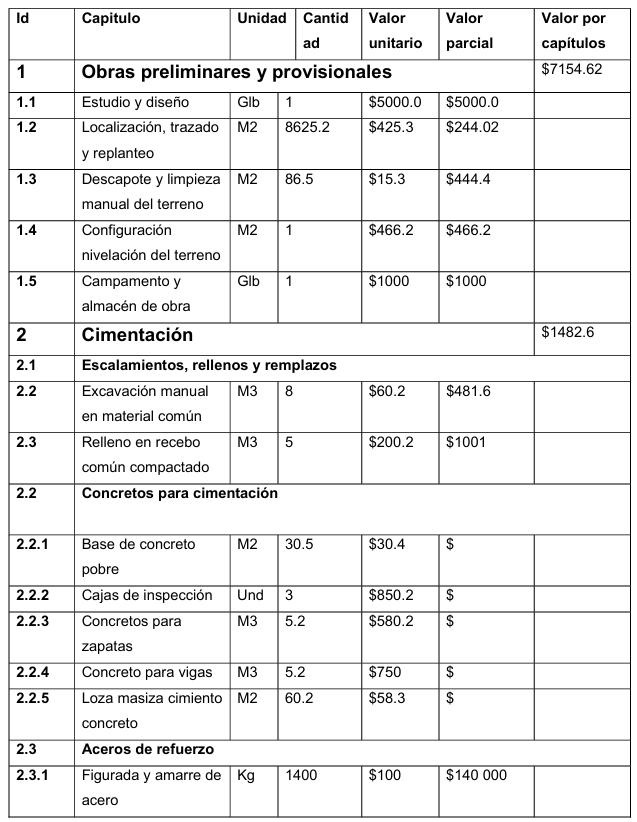
\includegraphics[width=1.0\textwidth]{chapters/ELC1.png} 
    \caption{Presupuesto de obra civil parte 1}
\label{fig:croquis190125}
\end{figure}

\begin{figure}[H]
    \centering	
    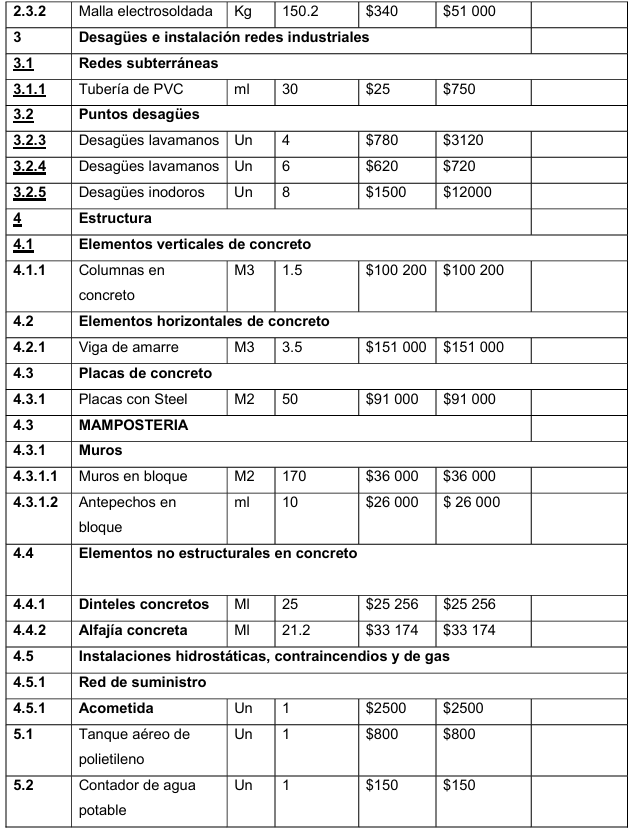
\includegraphics[width=1.0\textwidth]{chapters/ELC2.png} 
    \caption{Presupuesto de obra civil parte 2}
\label{fig:croquis190125}
\end{figure}

\begin{figure}[H]
    \centering	
    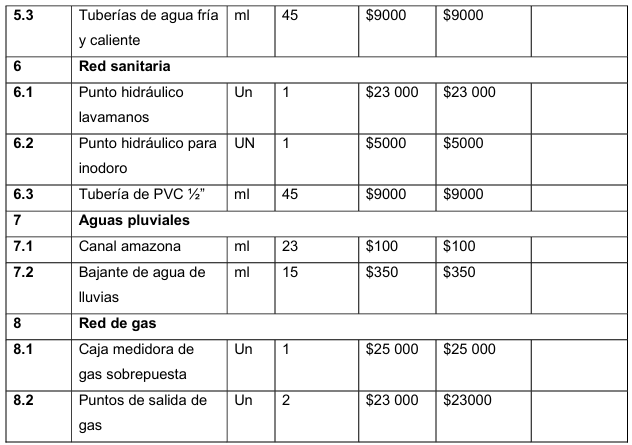
\includegraphics[width=1.0\textwidth]{chapters/ELC3.png} 
    \caption{Presupuesto de obra civil parte 3}
\label{fig:croquis190125}
\end{figure}


Para la construcción de la obra se tiene que invertir un aproximado de 3 251 125 pesos para poder tener la edificación y desde esta poder operar de manera adecuada y cómoda. 

%-------------------





\subsubsection{Adquisición de la tecnología de producción}

\begin{figure}[H]
    \centering	
    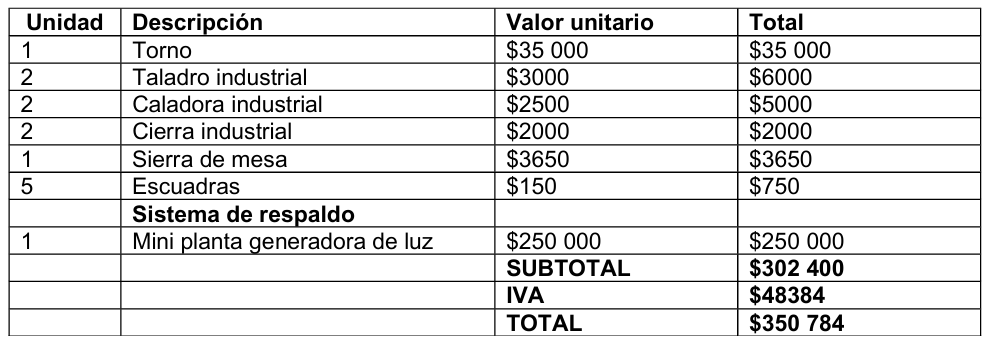
\includegraphics[width=1.1\textwidth]{chapters/ELC4.png} 
    \caption{Presupuesto de adquisición de tecnología }
\label{fig:croquis190125}
\end{figure}



\subsubsection{Adquisición de mobiliario y oficina}

\begin{figure}[H]
    \centering	
    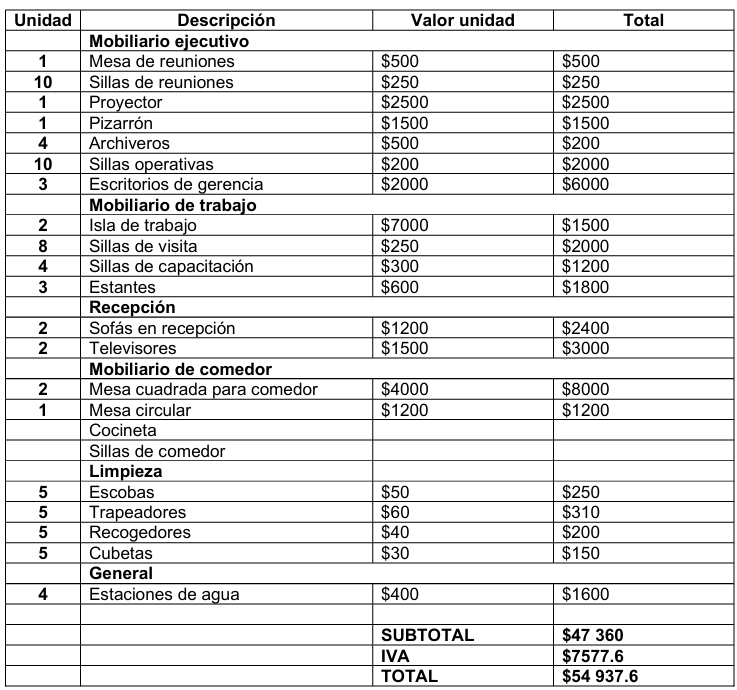
\includegraphics[width=1.1\textwidth]{chapters/ELC5.png} 
    \caption{Presupuesto de adquisición de mobiliario y oficina }
\label{fig:croquis190125}
\end{figure}

En la adquisición de mobiliario de oficina se tomo encuentra al mobiliario tanto de los ejecutivos, de los trabajadores, al que se colocaría en recepción, el comedor , la limpieza y generales ya que en cada uno de ellos se utilizan diferentes equipos de uso indispensable. 


\subsubsection{Adquisición del equipo de computo}

\begin{figure}[H]
    \centering	
    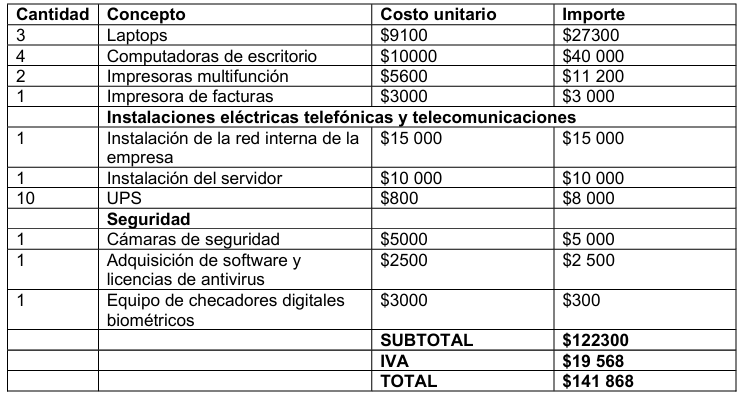
\includegraphics[width=1.1\textwidth]{chapters/ELC6.png} 
    \caption{Presupuesto de adquisición de mobiliario y oficina }
\label{fig:croquis190125}
\end{figure}






\subsection{Inversión diferida}
La inversión diferida se refiere a los gastos que una empresa realiza para obtener beneficios en el futuro, pero que no se consideran como activos fijos. Estos gastos no están destinados a adquirir activos físicos, sino que se utilizan para mejorar o mantener los activos existentes de una empresa.

Incluyen gastos en investigación y desarrollo, capacitación de empleados, publicidad, promoción y mejoras en la calidad de productos o servicios. Estos gastos son necesarios para mantener la competitividad de una empresa en el mercado y generar mayores ingresos en el futuro.

En los primeros momentos de producción no se espera invertir montos considerables en aspectos que no sean completamente necesarios para la producción, sin embargo se proponen las siguientes inversiones diferidas.

\begin{table}[h]
    \centering
    \caption{Inversión diferida bimestral}
    \begin{tabular}{p{5cm} || p{2cm} || p{3cm} || p{3cm}}
        \toprule
        \textbf{Concepto de Inversión Diferida} & \textbf{Precio mensual} & \textbf{Precio bimestral} & \textbf{Total bimestral}\\
        \midrule
        Capacitación de empleados & \$5,000 &\$10,000 &\\
        Mantenimiento de equipo & \$1,500 & \$3,000&\\
        Internet & \$1,000 & \$2,000&\\
        Luz & \$4,000 & \$8,000&\\
        Agua & \$600 & \$1,200 &\\
        Transporte & \$1,000 & \$2,000 &\\
        Publicidad & \$750 & \$1,500 &\\
        \hline
        IVA(16\%) & \$2,216 & \$4,432 & \$32,132\\
        \bottomrule
    \end{tabular}
\end{table}




\section{Depreciación y amortización}

\begin{figure}[H]
    \centering	
    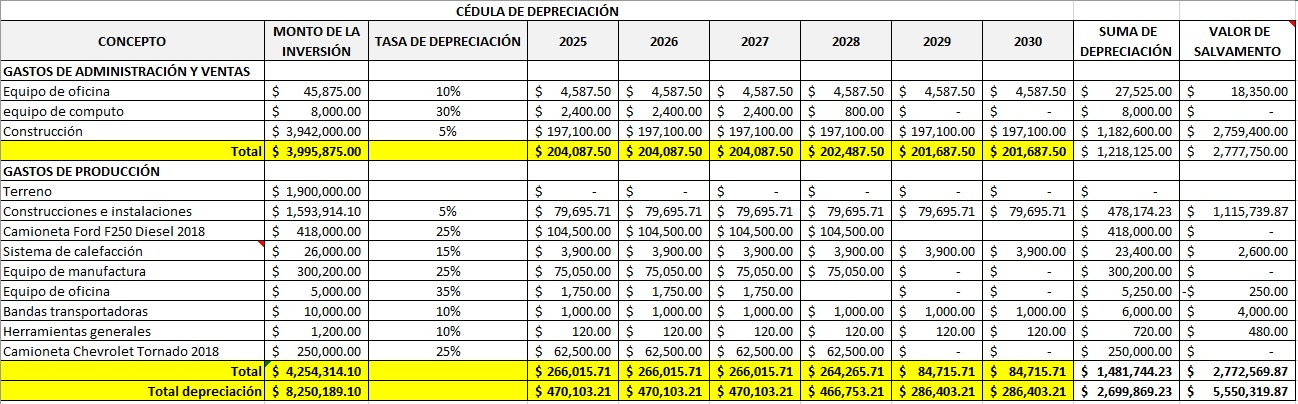
\includegraphics[width=1.1\textwidth]{chapters/ELC_10.png} 
    \caption{Célula de depreciación}
\label{fig:croquis190125}
\end{figure}



\section{Financiamiento de la inversión}

De los \$4 217 671.5 que se requieren de inversion fija y diferida, se pretende solicitar un prestamo por \$2 millones, el cual se liquidara en seis anualidades iguales, pagando la primera anualidad al final del primer año, por el cual se cobrará un interés de 32\% anual. Esta tasa de interés ya contiene a la inflación pronosticada. La anualidad que se pagará se calcula como:

La deuda equivalente a una aportación porcentual de capital de 47.149\%, por lo que la empresa deberá aportar el 52.58\% total sin incluir capital de trabajo. 

\begin{figure}[H]
    \centering	
    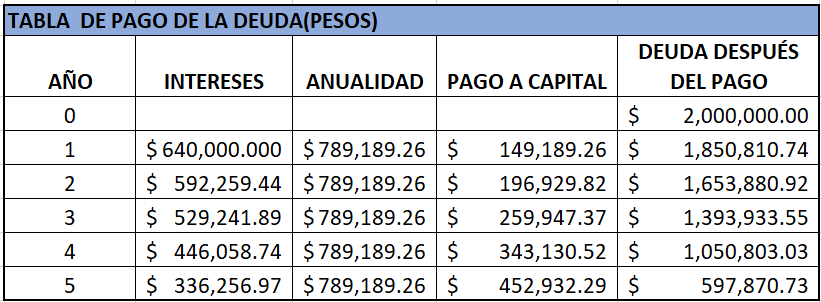
\includegraphics[width=0.9\textwidth]{chapters/ELC_11.png} 
    \caption{Tabla de pago de la deuda}
\label{fig:croquis190125}
\end{figure}


\section{Determinación del capital de trabajo Pasivo circulante}

\begin{table}[htbp]
    \centering
    \begin{tabular}{|l|c|c|c|}
        \hline
        \textbf{Concepto} & \textbf{Costo} & \textbf{IVA} & \textbf{Importe} \\
        \hline
        COSTO DE PRODUCCIÓN & & & \\
        \hline
        Materias primas & \$1000 & \$160 & \$1160 \\
        Materias primas secundarias y materiales indirectos & \$800 & \$128 & \$928 \\
        Sueldos y salarios & \$2500 & \$0 & \$2500 \\
        Gastos indirectos & \$1500 & \$0 & \$1500 \\
        \hline
        SUBTOTAL & & & \$6088 \\
        \hline
        GASTOS DE ADMINISTRACIÓN & & & \\
        \hline
        Sueldos y salarios & \$1000 & \$0 & \$1000 \\
        Gastos indirectos & \$800 & \$0 & \$800 \\
        \hline
        SUBTOTAL & & & \$1800 \\
        \hline
        GASTOS DE VENTA & & & \\
        \hline
        Sueldos y salarios & \$500 & \$0 & \$500 \\
        Gastos indirectos & \$300 & \$0 & \$300 \\
        \hline
        SUBTOTAL & & & \$800 \\
        \hline
        TOTAL & & & \$8688 \\
        \hline
    \end{tabular}
    \caption{Estimación del Capital de Trabajo}
    \label{tab:estimacion_capital_trabajo}
\end{table}

La tabla proporciona una estimación del capital de trabajo necesario para llevar a cabo el proyecto. Se divide en tres secciones principales: costo de producción, gastos de administración y gastos de venta.

En la sección de costo de producción, se detallan los diferentes elementos necesarios para la producción del sistema de control de planta, como materias primas, materiales indirectos y sueldos y salarios asociados con la producción. Además, se incluyen los gastos indirectos que pueden surgir durante este proceso. El subtotal muestra el total de estos costos de producción.

En la sección de gastos de administración, se enumeran los costos asociados con la gestión y administración del proyecto, incluidos los sueldos y salarios del personal administrativo y los gastos indirectos asociados con estas actividades. Nuevamente, se proporciona un subtotal para esta sección.

Finalmente, en la sección de gastos de venta, se presentan los costos relacionados con la promoción y comercialización del producto, como sueldos y salarios del personal de ventas y otros gastos indirectos relacionados con estas actividades. Se calcula un subtotal para esta sección.

El total general muestra la suma de todos los subtotales, proporcionando una estimación del capital de trabajo total necesario para llevar a cabo el proyecto. Esta tabla es útil para tener una idea general de los recursos financieros requeridos y planificar adecuadamente el presupuesto para el proyecto.


\section{Determinación del punto de equilibrio}

El punto de equilibrio es el nivel de producción en el que los ingresos por ventas son exactamente iguales a la suma de los costos fijos y los variables.

Ingresos= costo total

P × Q = CF + CV

Con base en el presupuesto de ingresos y de los costos de producción, administración y ventas, se clasifican los costos como fijos y variables, con la finalidad de determinar cuál es el nivel de producción donde los costos totales se igualan a los ingresos.


\begin{figure}[H]
    \centering	
    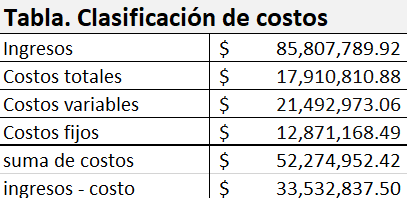
\includegraphics[width=0.6\textwidth]{chapters/ELC_PUNTO2.png} 
    \caption{Clasificación de costos}
\label{fig:croquis190125}
\end{figure}

\begin{figure}[H]
    \centering	
    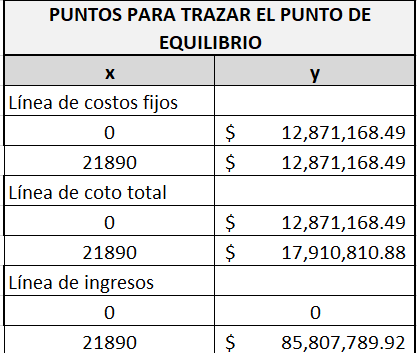
\includegraphics[width=0.6\textwidth]{chapters/ELC_PUNTO3.png} 
    \caption{Puntos para trazar el punto de equilibrio}
\label{fig:croquis190125}
\end{figure}


\begin{figure}[H]
    \centering	
    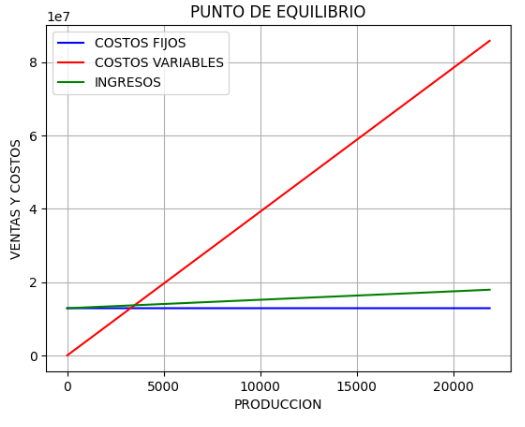
\includegraphics[width=0.9\textwidth]{chapters/ELC_PUNTO.png} 
    \caption{punto de equilibrio}
\label{fig:croquis190125}
\end{figure}



\section{Balance general inicial}

El balance general o balance de situación de una empresa es un documento contable financiero que refleja la situación económica y patrimonial de la misma en una fecha determinada, permite conocer la situación financiera y patrimonial de una compañía en un momento concreto, pues en él se detallan sus activos, sus pasivos y su capital.

La igualdad fundamental del balance:

	\textbf{	Activo = Pasivo + Capital }
  
\textbf{Activo}, representa cualquier pertenencia material o inmaterial de la empresa. 

\textbf{Pasivo} significa cualquier tipo de obligación o deuda que se tenga con terceros.

\textbf{Capital} significa los activos, representados en dinero o en títulos, que son propiedad de los accionistas o propietarios directos de la empresa.
A continuación se indica el cuadro del Balance General para el primer año de operación.

\begin{figure}[H]
    \centering	
    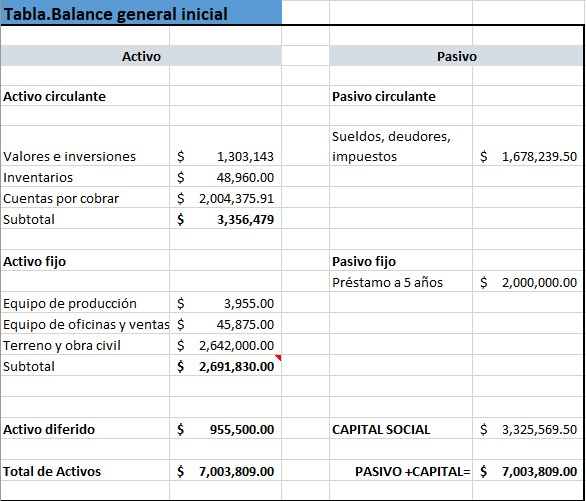
\includegraphics[width=0.9\textwidth]{chapters/ELC_12.png} 
    \caption{Balance general inicial}
\label{fig:croquis190125}
\end{figure}

El balance general inicial mostrará la aportación neta que deberán realizar los accionistas o promotores del proyecto. Notará que la aportación inicial de los accionistas es mucho mayor que los \$45 935 015 calculados para la inversión en activo fijo y diferido, ya que ahora se incluye el capital de trabajo. 

Generalmente para esta aportación adicional se solicita un crédito a corto plazo, recuerde que la naturaleza del capital de trabajo es a corto plazo, no más de tres o cuatro meses; por tanto, los intereses de este préstamo no aparecen en el estado de resultado.




\section{Estado de resultados pro-forma y su evaluación económica con VPN y TIR.}

El estado de resultados pro-forma o proyectado es la base para calcular los flujos netos de efectivo (FNE) con los cuales se realiza la evaluación económica.

Se presentarán tres estados de resultados, las cifras se redondean a miles de pesos; esto es una práctica aceptada cuando
se trabaja con cifras monetarias que se pretende se generen en el futuro.

\subsection{ Estado de resultados sin inflación, sin financiamiento y con producción constante. }

\begin{figure}[H]
    \centering	
    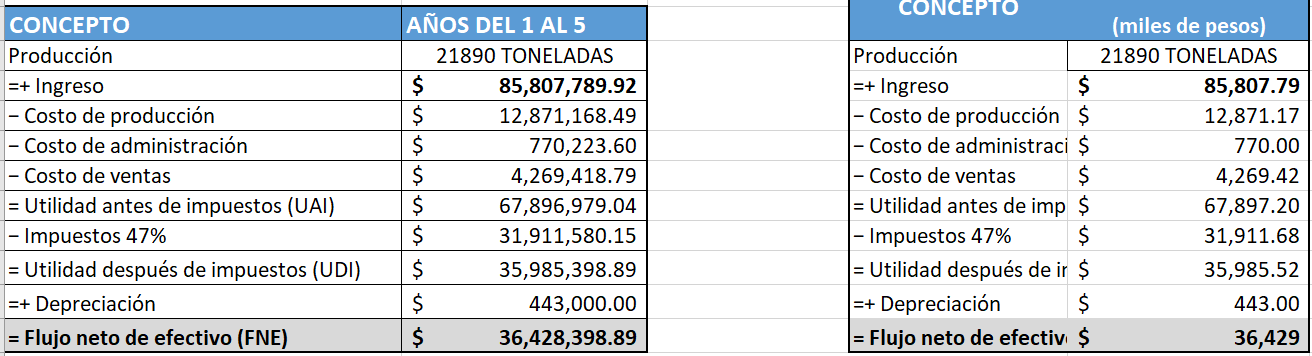
\includegraphics[width=1.1\textwidth]{chapters/ELC_13.png} 
    \caption{Tabla de estado de resultados sin inflación, sin financiamiento y con producción constante}
\label{fig:croquis190125}
\end{figure}

Como la producción es constante y no se toma en cuenta la inflación, entonces la hipótesis es considerar que las cifras de los flujos netos de efectivo se repiten cada fin de año durante todo el horizonte de análisis del proyecto.


\subsection{Estado de resultados con inflación, sin financiamiento y con producción constante.}

\begin{figure}[H]
    \centering	
    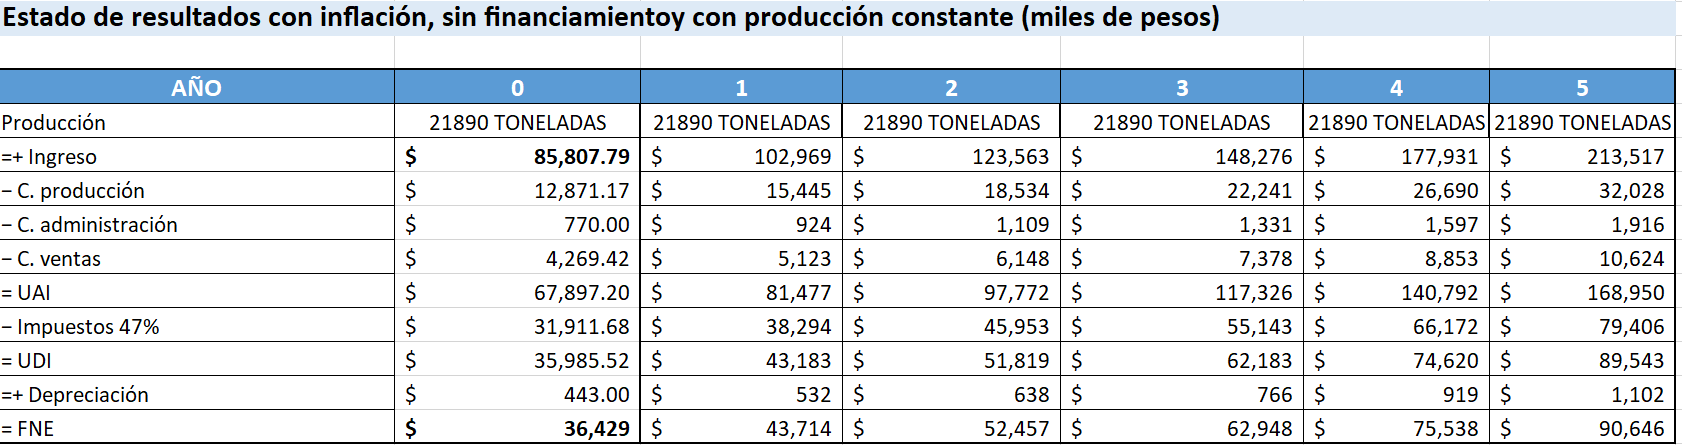
\includegraphics[width=1.1\textwidth]{chapters/ELC_14.png} 
    \caption{Tabla de estado de resultados con inflacón, sin financiamiento y con producción constante}
\label{fig:croquis190125}
\end{figure}

En el plateamiento del estado de resultados, el autor aplica un promedio del aumento de inflación anual de 20\%.  Y considera como el año cero el inicio de la producción para poder aplicar el efecto de la inflación en los años posteriores. Multiplica cada valor del año cero por 1.20.



\subsection{Estado de resultados con inflación, con financiamiento y con producción constante}


\begin{figure}[H]
    \centering	
    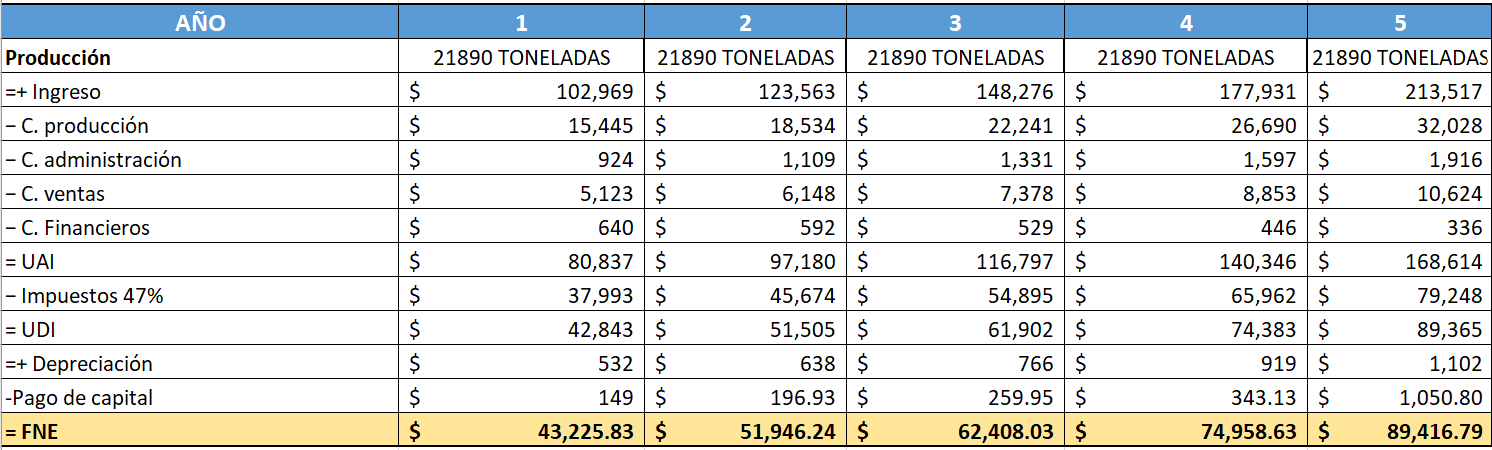
\includegraphics[width=1.1\textwidth]{chapters/ELC_15.png} 
    \caption{Estado de resulatados con inflación, con financiamiento y con roducción constante}
\label{fig:croquis190125}
\end{figure}

 \section{Cálculo del VPN y la TlR con producción variable, sin inflación, con financiamiento}

 \begin{figure}[H]
    \centering	
    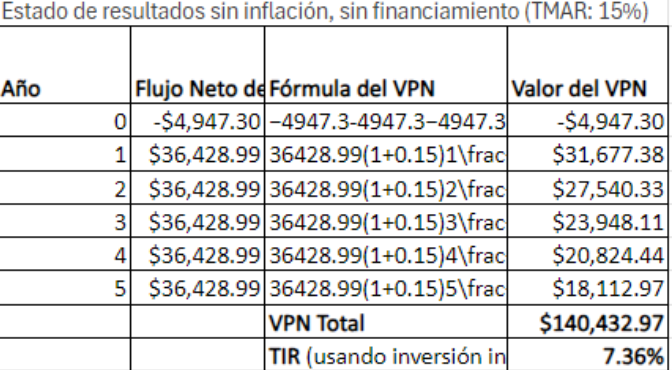
\includegraphics[width=0.7\textwidth]{chapters/ELC_16.png} 
    \caption{Estado de resultados sin inflación,sin financiamiento}
\label{fig:croquis190125}
\end{figure}

\begin{figure}[H]
    \centering	
    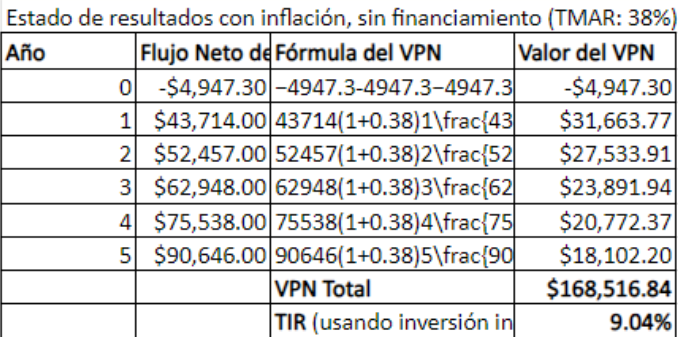
\includegraphics[width=0.7\textwidth]{chapters/ELC_17.png} 
    \caption{Estado de resultados con inflación,sin financiamiento}
\label{fig:croquis190125}
\end{figure}

\begin{figure}[H]
    \centering	
    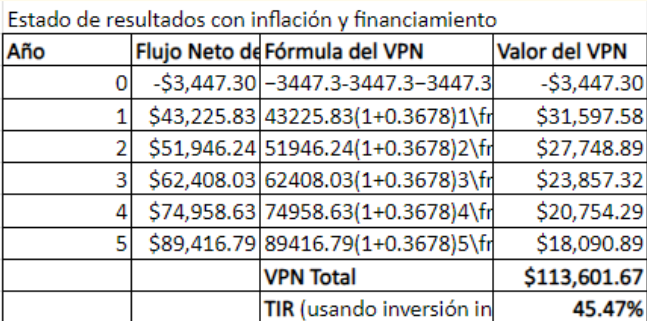
\includegraphics[width=0.7\textwidth]{chapters/ELC_18.png} 
    \caption{Estado de resultados con inflación y financiamiento}
\label{fig:croquis190125}
\end{figure}


\section{Cronograma de inversiones}

Se decidió que el tiempo deseado desde la planeación a la apertura de la empresa sea de 6 meses, por lo que se propone el siguiente calendario. 

\begin{figure}[H]
    \centering	
    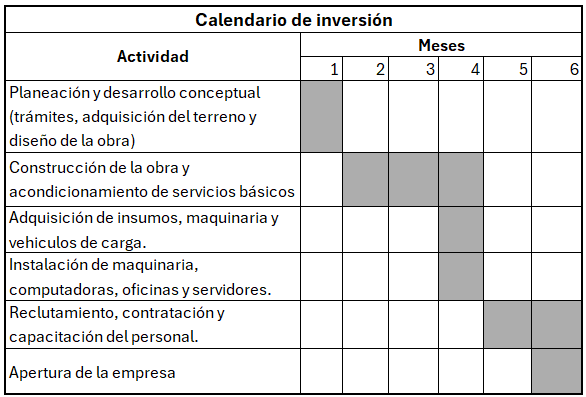
\includegraphics[width=.8\textwidth]{img/Calendario de inversion.png} 
    \caption{Calendario de inversión}
\label{fig:calendarioInversion}
\end{figure}

El calendario está previsto de la siguiente manera sin embargo el reclutamiento y la capacitación del personal se podría adelantar un mes ya que se podrían impartir lecciones teóricas del funcionamiento. 

\section{Conclusiones del estudio económico y evaluación económica}



 El análisis muestra que el proyecto es rentable con un retorno de inversión positivo. Las proyecciones financieras indican que los ingresos generados superarán los costos operativos y de inversión inicial en un plazo razonable.
 Los beneficios derivados de la mejora en la calidad y la cantidad de la producción de flores superan los costos de instalación y operación de las cámaras climáticas.

Se estima que el periodo de recuperación de la inversión inicial es de 5 años, lo cual es aceptable dentro del sector agrícola.
Las proyecciones de ingresos muestran un crecimiento sostenido a lo largo del tiempo, con un aumento en la rentabilidad conforme se estabiliza la operación de las cámaras climáticas.

El análisis detalla los costos iniciales de adquisición e instalación de las cámaras climáticas, así como los gastos en infraestructura y tecnología.

El estudio económico y la evaluación económica del proyecto de cámaras climáticas para flores demuestra que el proyecto es financieramente viable y tiene un potencial significativo para mejorar la producción y calidad de las flores. A través de la implementación de tecnologías avanzadas y prácticas eficientes, el proyecto puede generar beneficios sustanciales tanto para los inversores como para la comunidad local. Además, la capacidad de mitigar riesgos y adaptarse a diferentes escenarios económicos asegura la sostenibilidad a largo plazo del proyecto.
\include{chapter/Conclusiones.tex}


%Without the word "section"
\fancyhead[LO]{\nouppercase{\rightmark}} 
%Añadimos las referncias
\printbibliography[title=Referencias]

\chapter{Anexos}
\section{Resultados de la encuesta}
Los principales datos para analizar de la encuesta realizada son:

\begin{figure}[H]
    \centering	
    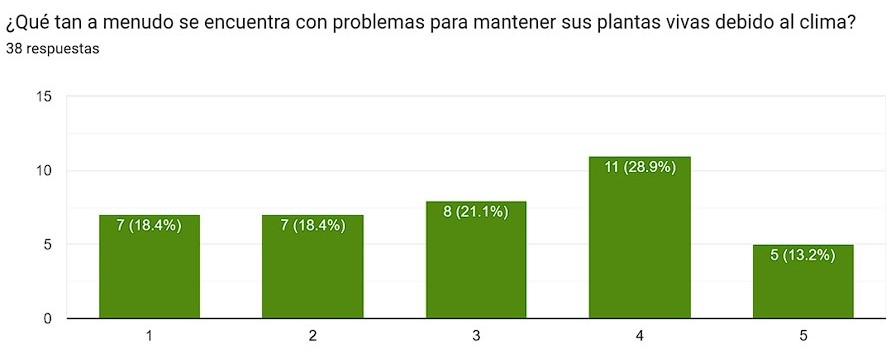
\includegraphics[width=.8\textwidth]{img/Empresa/encuesta1.jpg} 
    \caption{Problemas para mantener con vida sus plantas}
\label{fig:encuesta1}
\end{figure}

El porcentaje de personas que presentan problemas para mantener sus plantas vivas por el clima ver figura \ref{fig:encuesta1}.

\begin{figure}[H]
    \centering	
    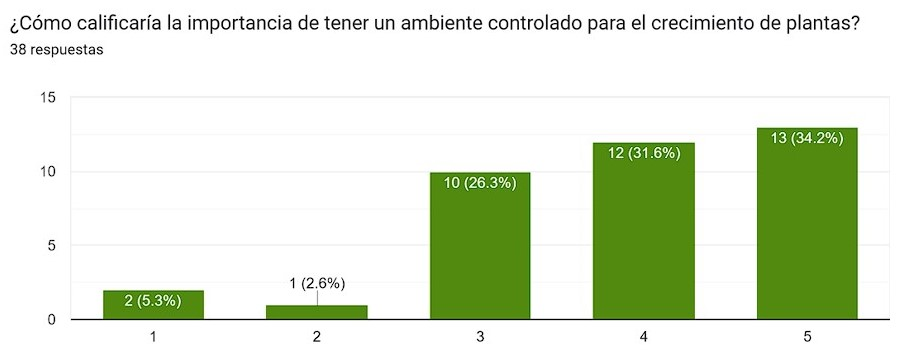
\includegraphics[width=.8\textwidth]{img/Empresa/encuesta2.jpg} 
    \caption{Importancia de ambiente controlado}
\label{fig:encuesta2}
\end{figure}

Percepción de la importancia de controlar el ambiente para el correcto crecimiento de plantas ver figura \ref{fig:encuesta2}.

\begin{figure}[H]
    \centering	
    \includegraphics[width=.8\textwidth]{img/Empresa/encuesta3.jpg} 
    \caption{Importancia por tipos de planta}
\label{fig:encuesta3}
\end{figure}

Es importante recalcar que más del 40\% de los encuestados utilizarían el producto con fines de reforestación y producción de alimentos, incluso con mayor porcentaje de la población que la utilizaría en su casa u oficina ver figura \ref{fig:encuesta3}.

\begin{figure}[H]
    \centering	
    \includegraphics[width=.8\textwidth]{img/Empresa/encuesta4.jpg} 
    \caption{Rango de precios}
\label{fig:encuesta4}
\end{figure}

\section{Requisitos Municipales}
\label{sec:requisitosMunicipales}
\includepdf[pages=-]{chapters/RequisitosMunicipales.pdf}

%\include{chapters/c_metodologia}
%\include{chapters/disenoPreliminar}
%\include{chapters/d_resultados}
%\include{chapters/e_discussao}
%%% ------------------------------------------------------------------------- %%
\chapter{Análisis de resultados}
\label{aresultados}
En este capítulo se analizarán los resultados obtenidos hasta ahora, si bien no se ha terminado de culminar el proyecto, se mostrarán algunos de los resultados preliminares, tomando estos resultados como retroalimentación para mejorar los sistemas.

\begin{figure}[H]
    \centering	
    \includegraphics[width=.8\textwidth]{img/Figure_1.png} 
    \caption{Gráfica de estabilidad del sistema, ángulo deseado vs tiempo}
	\label{fig:simulacionControlPython}
\end{figure}

La figura  \ref{fig:simulacionControlPython} muestra una gráfica obtenida de un programa que se ha realizado en Python en conjunto con la interfaz (figura \ref{fig:simulacionControlPython2}), en este programa se ingresa un ángulo deseado, el cual es enviado a través del puerto serial a la unidad de procesamiento, en este caso es un ESP32, una vez enviado el ángulo este comienza a activar los motores a diferentes velocidades con el objetivo de estabilizar el sistema en el ángulo proporcionado. Como se observa en la imagen, el algoritmo de control no cumple con su objetivo, ya que simplemente oscila y no logra mantener la estabilidad dada en el ángulo dado.

\begin{figure}[H]
    \centering	
    \includegraphics[width=.8\textwidth]{img/Control.jpg} 
    \caption{Programa de Python con interfaz y gráfica de estabilidad en tiempo real}
	\label{fig:simulacionControlPython2}
\end{figure}

Esto sucede ya que el control fuzzy implementado contempla valores de 0 a 255, que son parámetros del ancho de pulso que requiere el puente H de los motores, sin embargo los motores solo se activan hasta tener un ancho de pulso mayor a 150, por lo que es necesario cambiar de controlador, que englobe valores más altos y ya no menores al valor dicho.
Estos cambios se agregarán más adelante y se compararán con estos, para tener una mejor idea de como ha mejorado el controlador.

\begin{figure}[H]
    \centering	
    \includegraphics[width=.8\textwidth]{img/Rplot.png} 
    \caption{ Gráfica de estabilidad del sistema final}
	\label{fig:simulacionControlR}
\end{figure}

%------------------------------------------------------
\newpage
\section{Análisis de costos} 
En esta sección se analizarán los gastos directos, indirectos, la amortización así como el precio total del proyecto.
%------------------------------------------------------

\textbf{Costos directos}

\begin{table}[H]
\centering
\caption{Costos directos}
\begin{tabular}{p{4cm}|p{4cm}|p{4cm}}
\hline
\textbf{Componentes / Insumos }& \textbf{Cantidad} & \textbf{Costos} \\
\hline
Cabina de unicel&1&\$190\\
\hline
Escudo térmico, insulation&1 rollo&\$470\\
\hline
Filamento fibra de carbono&1&\$700\\
\hline
ESP32&2&\$300\\
\hline
Sensor de presión barométrica y temperatura&1&\$50\\
\hline
Placas de baquelita de 10x10 cm&1 paquete&\$160\\
\hline
Giroscopio MPU6050&1&\$65\\
\hline
Modulo GPS&1&\$200\\
\hline
Regulador de voltaje&1&\$45\\
\hline
Módulo GSM&1&\$140\\
\hline
Bateria lipo, 3s 1600mAh&1&\$700\\
\hline
Sensor humedad&1&\$165\\
\hline
Driver DRV8833&1&\$140\\
\hline
Hélices par&1&\$200\\
\hline
Cables estañados, calibre 22&1&\$220\\
\hline
Conectores JST-XH 2.0 mm&1&\$100\\
\hline
\textbf{Total:} & &\textbf{3845}\\

\hline
\end{tabular}
\label{tabla:costosDirectos}
\end{table}

%-----------------------------------------------------

\textbf{Costos indirectos}

\begin{table}[H]
\centering
\caption{Costos indirectos}
\begin{tabular}{p{6cm}|p{4cm}}
\hline
\textbf{Servicios } & \textbf{Costo} \\
\hline
Renta de servicio de luz &\$600\\
\hline
Insumos de alimentos&\$2000\\
\hline
Renta de internet&\$800\\

\hline
\end{tabular}
\label{tabla:costosIndirectos}
\end{table}

%-----------------------------------------------------
\textbf{Amortización}

La amortización es un concepto contable que hace referencia a la pérdida de valor de un bien durante su vida útil. Se registra con la intención de reflejar el valor real de una propiedad, considerando el uso, desgaste y valor residual. 

\begin{figure}[H]
    \centering	
    \includegraphics[width=.9\textwidth]{img/amortizacion.jpg} 
    \caption{ Amortización del producto}
	\label{fig:amortizacion}
\end{figure}

%-----------------------------------------------------



% Prints a list of abbreviations
%\chapter{Anexos}
\section{Resultados de la encuesta}
Los principales datos para analizar de la encuesta realizada son:

\begin{figure}[H]
    \centering	
    \includegraphics[width=.8\textwidth]{img/Empresa/encuesta1.jpg} 
    \caption{Problemas para mantener con vida sus plantas}
\label{fig:encuesta1}
\end{figure}

El porcentaje de personas que presentan problemas para mantener sus plantas vivas por el clima ver figura \ref{fig:encuesta1}.

\begin{figure}[H]
    \centering	
    \includegraphics[width=.8\textwidth]{img/Empresa/encuesta2.jpg} 
    \caption{Importancia de ambiente controlado}
\label{fig:encuesta2}
\end{figure}

Percepción de la importancia de controlar el ambiente para el correcto crecimiento de plantas ver figura \ref{fig:encuesta2}.

\begin{figure}[H]
    \centering	
    \includegraphics[width=.8\textwidth]{img/Empresa/encuesta3.jpg} 
    \caption{Importancia por tipos de planta}
\label{fig:encuesta3}
\end{figure}

Es importante recalcar que más del 40\% de los encuestados utilizarían el producto con fines de reforestación y producción de alimentos, incluso con mayor porcentaje de la población que la utilizaría en su casa u oficina ver figura \ref{fig:encuesta3}.

\begin{figure}[H]
    \centering	
    \includegraphics[width=.8\textwidth]{img/Empresa/encuesta4.jpg} 
    \caption{Rango de precios}
\label{fig:encuesta4}
\end{figure}

\section{Requisitos Municipales}
\label{sec:requisitosMunicipales}
\includepdf[pages=-]{chapters/RequisitosMunicipales.pdf}

%\chapter{Referéncias}

NASA, (DSCOVR: EPIC,) 16 10 2023. [En línea]. Available: https://epic.gsfc.nasa.gov/.

NASA, (eclipse,) 16 10 2023. [En línea]. Available: https://eclipse.gsfc.nasa.gov/SEdecade/SEdecade1991.html.
D. B. C. T. Amir Caspi, (arxiv,) 1 Junio 2020. [En línea]. Available: https://arxiv.org/abs/2004.09658. [Último acceso: 16 Octubre 2023].

Exploratorium, (Exploratorium,) 15 10 2023. [En línea]. Available: https://www.exploratorium.edu/es/eclipse/por-qu%C3%A9-estudiamos-los-eclipses-solares.

T. Humphrey, «bbc,» 14 7 2019. [En línea]. Available: https://www.bbc.com/news/uk-england-hampshire-66188381.

V. G. A. M. Lugo Gozález, «Mechatronic design implemented in the development of virtual and physical prototypes,» Diciembre 2020. [En línea]. Available: https://www.researchgate.net/publication/348209704_Diseno_mecatronico_implementado_en_el_desarrollo_de_prototipos_virtuales_y_fisicos_Mechatronic_design_implemented_in_the_development_of_virtual_and_physical_prototypes. [Último acceso: 03 Noviembre 2023].

C. J. L. O. A. L. d. M. C. Jiménez Fernández, «Redalyc,» Diciembre 2010. [En línea]. Available: http://www.redalyc.org/articulo.oa?id=36815118002. [Último acceso: 03 Noviembre 2023].

S. Laoyan, «asana,» 29 septiembre 2022. [En línea]. Available: https://asana.com/es/resources/waterfall-project-management-methodology. [Último acceso: 03 Noviembre 2023].

M. Kramer, «space,» 02 Febrero 2015. [En línea]. Available: https://www.space.com/28481-spacex-launches-dscovr-satellite.html. [Último acceso: 15 Octubre 2023].
zkl, «zkl doc,» [En línea]. Available: https://blog.zerokol.com/2012/09/arduinofuzzy-uma-biblioteca-fuzzy-para.html. [Último acceso: 1 Diciembre 2023].
E. C. Alvarez, «Mexico desconocido,» 15 10 2023. [En línea]. Available: https://www.mexicodesconocido.com.mx/eclipses-yucatan-cultura-maya-aztecas.html.
NESDIS, «National Environmental Satellite, Data and Information Service.,» 16 10 2023. [En línea]. Available: https://www.nesdis.noaa.gov/current-satellite-missions/currently-flying/dscovr-deep-space-climate-observatory.
NASA, «cubesat,» 16 10 2023. [En línea]. Available: https://www.cubesat.org/past-launches/2017-delta-ii-jpss-1-elana14.
F. Meconi, «Terraza al cosmos,» 2020. [En línea]. Available: https://www.terrazaalcosmos.com.ar/eclipsor.
El mundo Madrid, «El mundo,» 22 Junio 2016. [En línea]. Available: https://www.elmundo.es/ciencia/2016/06/22/576abf57268e3ebc3f8b45ed.html. [Último acceso: 20 10 2023].
NASA, «EPIC,» 14 Octubre 2023. [En línea]. Available: https://epic.gsfc.nasa.gov/enhanced?date=2023-10-14. [Último acceso: 16 Octubre 2023].


% Prints a list of symbols
%\chapter*{Lista de Símbolos} 
\addcontentsline{toc}{chapter}{Lista de Símbolos}

\begin{longtable}[l]{l l} 
   \textbf{Símbolo}	& \textbf{Descrição} \\
   
   $\omega$ & Frequência angular \\
   $\psi$ & Função de análise wavelet \\ 
   $\pi$ &  Número pi\\
   ... & ... \\ 
\end{longtable}

% To start appendices with different chapter numbering
%\appendix

%\fancyhead[LO]{\nouppercase{\rightmark}} 


\end{document}